
\documentclass[letterpaper,twocolumn,10pt]{article}
\usepackage{usenix2019_v3}
\usepackage{algorithmic}
\usepackage{algorithm}
\usepackage{listings}
\usepackage{pifont}
\usepackage{multirow}
\usepackage{graphicx}
\usepackage{caption}
\usepackage{xcolor}
\usepackage{booktabs}

% to be able to draw some self-contained figs
\usepackage{tikz}
\usepackage{amsmath}
\usepackage{cleveref}
\usepackage{subcaption}
\crefname{section}{§}{§§}
\Crefname{section}{§}{§§}

% new commands
\newcommand{\name}{CATFlow}

\newcommand{\junfeng}[1]{{\color{blue}[Junfeng: #1]}}
\newcommand{\weihao}[1]{{\color{red}[Weihao: #1]}}
\newcommand{\huanyu}[1]{{\color{orange}[Huanyu: #1]}}
\newcommand{\todo}[1]{{\color{purple}TODO: #1}}
\newcommand{\new}[1]{{\color{purple}New version: #1}}
\newcommand{\old}[1]{{\color{orange}Old version: #1}}

% \newcommand{\junfeng}[1]{{\color{blue}}}
% \newcommand{\huanyu}[1]{{\color{blue}}}
% \newcommand{\weihao}[1]{{\color{blue}}}
% \newcommand{\todo}[1]{{\color{purple}}}
% \newcommand{\new}[1]{{\color{purple}}}
% \newcommand{\old}[1]{{\color{orange}}}

%-------------------------------------------------------------------------------
\begin{document}
%-------------------------------------------------------------------------------

%don't want date printed
\date{}

% make title bold and 14 pt font (Latex default is non-bold, 16 pt)
\title{\Large \bf \name{}: Data-Monistic Parallelization Plan Discovery for Distributed Training}

%for single author (just remove % characters)
\author{
% {\rm Your N.\ Here}\\
% Your Institution
% \and
% {\rm Second Name}\\
% Second Institution
% % copy the following lines to add more authors
% % \and
% % {\rm Name}\\
% %Name Institution
} % end author

\maketitle

%-------------------------------------------------------------------------------
\begin{abstract}
%-------------------------------------------------------------------------------
As neural networks grow in size and complexity, distributed training across multiple devices becomes essential. An expressive abstraction is crucial for describing diverse parallelism paradigms to maximize hardware resource utilization. However, prevailing operator-centric abstractions fall short, as they fail to describe complex data movement optimizations and precise data lifecycle management, and cannot support the automatic discovery of new parallelism paradigms.

In this paper, we introduce \name{}, a novel abstraction that presents a key insight: defining parallelism spaces from a pure data-centric perspective offers greater expressiveness and completeness than operator-centric approaches. \name{} is built upon three fundamental representations: tensors, space-time coordinates, and their relationships, formalized as constraints. It also provides a set of primitives for constructing and manipulating these elements, enabling the description of diverse operator schedules and the co-optimization of computation and data movement. A key advantage of \name{} is its capacity to explicitly encode constraints on spatial dataflow trajectories and tensor lifecycles through these primitives to form a search space for parallelism paradigms. This facilitates systematic searches within this constrained optimization space to discover new, efficient parallelism paradigms. Using a constraint-based potential descent algorithm, we have discovered novel training solutions with \name{}, such as ZeRO-3.5 and ZeRO-4, which achieve the low memory footprint of ZeRO-3 with better performance, delivering up to 39.1\% performance improvement (ZeRO-3) and 36.6\% less memory (ZeRO-2) across hardware configurations, and new offloading strategies that boost throughput by up to 89.4\%.

\end{abstract}

\section{Introduction}
\label{sec:intro}

% 明确一下名词
% strategy space -> strategy -> plan. Strategy space包含了多个strategy
% 而plan是一个具体的并行实现方式。对于传统的方法，确定了一个strategy的参数之后，就会得到一个plan
% 本文的路径 strategy space -> strategy 与传统路径是有一定冲突的，所以我们将传统路径描述为stategy template -> plan
% 不要说implementation，implementation是指我们系统的工程实现方式。比如说用的Python构建接口啊等等
% 另一个小问题：operators准确的说是不是computation及其相关的storage -> 是的
Deep Neural Networks (DNNs), particularly large language models (LLMs), have achieved advanced performance across a wide range of domains at the cost of increasing model sizes. Consequently, distributing training across multiple devices is crucial. The core challenge lies in identifying an efficient parallelization plan for distributed training. An NN model can be formally modeled as a dataflow graph~\cite{lin2023songc}, where nodes represent either data storage (tensors) or computations (operators), and directed edges represent dependencies between nodes. A comprehensive parallelization strategy specifies the distribution and scheduling of storage and computation in both space (device placement) and time (execution order)~\cite{qiu2025moirai, huang2019yugong, lin2024nnscaler}. The space of feasible parallelization plans is vast, and the problem of determining an optimal plan is NP-hard~\cite{liu2024aceso}.

Due to the immense search space and complex constraints, distributed training optimizations often rely on meticulously designed paradigms that incorporate domain expertise. Examples include Megatron-LM~\cite{shoeybi2019megatron, narayanan2021efficient}, which incorporates parameterized parallelism mechanisms known as data, tensor, and pipeline parallelism (DP, TP, PP, collectively termed 3D parallelism) to support Transformer-based models. Alternatively, systems like Piper~\cite{tarnawski2021piper} and Alpa~\cite{zheng2022alpa} adopt a hierarchical search, first determining a plan for pipeline (inter-operator) parallelism, then optimizing tensor (intra-operator) parallelism within each stage. A common pattern across these methods is to first define a specific parallelism paradigm (e.g., 3D or SPMD parallelism) and then perform an efficient hyperparameter search within that paradigm—for instance, tuning the degrees of data, tensor, and pipeline parallelism.

\begin{table*}[t!]
\small
\centering
\setlength{\tabcolsep}{4pt}
\caption{High-level comparison of paradigms.}
\label{tab:landscape}
\begin{tabular}{p{0.14\linewidth}p{0.26\linewidth}p{0.26\linewidth}p{0.26\linewidth}}
\toprule
\textbf{Feature} & \textbf{Classical} (e.g., Megatron-LM) & \textbf{nnScaler} & \textbf{\name{}} \\
\midrule
\textbf{Fundamental view} & \textbf{Strategy-centric:} fixed library of named strategies (e.g., DP, PP, TP) & \textbf{Operator-centric:} define strategy by operator behaviors & \textbf{Data-monistic:} define strategy by data trajectories \\
\textbf{Space definition / Prim. semantics} & \textbf{Fixed templates:} combination of existing strategies (e.g., 1F1B, 3D) & \textbf{Constructive:} default-deny, explicitly permit; build form zero. & \textbf{Subtractive:} default-allow, explicitly forbid; carve from universal set\\
\textbf{Completeness} & \textbf{Low:} combination of built-ins & \textbf{Medium:} complete for computation scheduling & \textbf{High:} covering computation, storage, and communication co-optimization \\
\textbf{Expressiveness} & \textbf{Low:} combination rules of built-ins & \textbf{Medium:} custom operator schedules, no data-centric optimizations. & \textbf{High:} fine-grained control over tensor life-cycle and events \\
\textbf{Searchability} & \textbf{Parameter search} & \textbf{Para. search in user-defined space} & \textbf{Automatic strategy discovery} \\
\textbf{Dataflow handling} & Implicit and fixed by chosen strategy & Implicit side-effect of operator & Explicit and first-class target \\
\bottomrule
\end{tabular}
\end{table*}

While many studies~\cite{tarnawski2021piper, zheng2022alpa, liu2024aceso} focus on specific plan searches within different strategy classes, recent work~\cite{lin2024nnscaler, lin2024tessel} advocates domain-specific primitives that allow experts to construct customized strategies. This paradigm recognizes that variations in hardware, workload characteristics, and expert knowledge can lead to distinct preferred strategies, thus providing a more flexible framework to unlock further optimization opportunities. Experts define novel strategies with their designed patterns and search configurations.

However, existing approaches still face two limitations. First, they either define rigid strategy spaces or lack completeness in strategy specification, making it hard to capture more potential opportunities. Although nnScaler~\cite{lin2024nnscaler} represents a significant advance in strategy construction—capable of describing most existing training plans and new expert-crafted strategies—it remains unable to express optimizations involving coordinated data movement, such as ZeRO~\cite{rajbhandari2020zero} and WeiPipe~\cite{lin2025weipipe}, thus hindering the ability to fully exploit hardware resources. Second, the quality of this pre-designed space is a critical determinant of the achievable performance of these frameworks, which are limited to automated search within a fixed strategy space; search algorithms select among efficient configurations and parameter settings (e.g., partition sizes, device assignments, execution order) rather than enabling the automatic discovery of unforeseen strategies.

For methods that define strategies using domain-specific primitives, their expressiveness is constrained by the underlying abstractions and specifications. Existing approaches are predominantly operator-centric. For instance, nnScaler~\cite{lin2024nnscaler} introduces three primitives—\texttt{op-trans}, \texttt{op-assign}, and \texttt{op-order}—for specifying operator behaviors. These approaches focus on computation and implicitly bind default data movement to operator scheduling. We present a core contrary insight: adopting a \textbf{data-monistic} perspective yields a more expressive and complete abstraction for strategy-space construction, in which parallelization plans are defined by describing the trajectory of data and imposing constraints on its movement. From this viewpoint, computation is implicitly represented as a \textbf{constraint} on dataflow; that is, its occurrence means all required data must meet at the same device, and the scheduling of computation can be deduced naturally from the constraints that govern data movement.

Building on this insight, we present \name{}—a framework for describing, generating, and searching for distributed-training plans. Its core is an abstraction centered on constraint-aware tensors (CATs). The constraints associated with each tensor specify its space-time coordinates (when and where a tensor resides). \name{} provides a set of primitives for manipulating CATs to constrain strategies that coordinate data movement and computation.

% \begin{table*}[t]
% \small
% \centering
% \setlength{\tabcolsep}{4pt}
% \caption{High-level comparison of paradigms.}
% \label{tab:landscape}
% \begin{tabular}{llll}
% \toprule
% Feature & Traditional & nnScaler & \name{} \\
% \midrule
% Fundamental view & Strategy-centric & Operator-centric & Data-monistic \\
% Space definition & Fixed templates & Constructive & Declarative \\
% System role & Parameter search & Template search & Strategy discovery \\
% Expressiveness & Low (built-ins) & Medium (op-schedules) & High (data \& op) \\
% Dataflow handling & Implicit & Implicit & Explicit \\
% \bottomrule
% \end{tabular}
% \end{table*}

Unlike pre-designed strategy spaces, \name{} employs declarative, subtractive primitives to carve a \textit{universal} strategy space through constraints. Prior approaches rely on constructive primitives to explicitly specify scheduling behavior, requiring users to design what a policy should be. In contrast, \name{}'s reductive methods allow designers to stipulate what a policy should not be. The resulting strategy space therefore encompasses both established and unforeseen designs, thereby opening opportunities for strategy discovery. Further, the data-monistic perspective provides a unified, high-resolution landscape that improves optimization tractability and supports smooth transitions between plans during search. Building on these foundations, we propose a constraint-based potential descent algorithm that discovers novel parallelization strategies beyond parameter tuning. Table~\ref{tab:landscape} summarizes the key differences between \name{} and others.

\name{}'s core contributions are summarized as follows:

1. \textbf{Data-Monistic Parallelization Strategy Abstraction and Space Construction:} We introduce \name{}, a framework featuring novel abstractions and primitives for constructing parallelization strategy spaces in distributed NN training. \name{} enables the explicit and complete specification of strategies involving both computation and data movement from a data-monistic view. This stands in contrast to existing operator-centric approaches, unlocking a strictly larger and more expressive strategy space.

2. \textbf{Automatic Discovery of Novel Strategies:} Leveraging \name{}'s unified abstractions, a strategy space can be reductively carved by constraining CATs. Within the strategy space, we propose a potential descent algorithm that enables the automatic discovery of unforeseen parallelization strategies, going beyond traditional parameter search within a fixed strategy pattern.

3. \textbf{Presentation of New Strategies:} Based on \name{}, we present new, efficient distributed training strategies for resource-constrained scenarios that match or surpass state-of-the-art, manually designed solutions. These include a novel strategy that achieves the memory efficiency of ZeRO-3 and performance approaching that of ZeRO-2, as well as delivering near-linear scaling and improved hardware utilization.

\section{Background \& Motivation}

\subsection{Search Space for Parallelization Plans}

% 首先说有很大的搜索空间
% 然后介绍了了DP, TP, PP以及3D并行
% 介绍一下Tessel的PP, Megatron的3D并行search space, Alpa和Piper的staged SPMD
% 介绍一下exiting search spaces存在limitations, 这样的predefined的search space是针对固定的workload准备的, 对于更大范围的workload来说，不够通用，会丢掉很多优化机会，比如说AlphaFold2的3F1B和embedding层的low computation utilization问题

A \textit{parallelization plan} specifies how a model is partitioned and scheduled across multiple devices, including the distribution of tensors (data), operators (computations), and their temporal order. The challenge lies in the vast combinatorial space of possible plans, and finding the optimal plan is NP-hard. Most approaches use either handcrafted parallelization plans or constrained search spaces. Common strategies include:

\textit{Data Parallelism:} Replicates operators across devices, partitioning the input batch. Each replica processes a portion of the batch and shares model parameters. \textit{Tensor Parallelism:} Partitions operators and tensors along dimensions beyond the batch, enabling distribution of a single operator across devices—crucial for models exceeding single-device memory. \textit{Pipeline Parallelism:} Divides the model into sequential stages assigned to device meshes and executed in a pipelined fashion. The input batch is split into micro-batches, processed in a scheduled order. These strategies are often combined as \textit{3D Parallelism}. Megatron-LM~\cite{} exemplifies this, combining DP, TP, and PP for Transformer models. Piper and Alpa extend this with staged SPMD, first searching for a PP strategy, then an SPMD plan within each stage (Alpa allows more flexible TP configurations). While effective, these approaches often fix schedules like 1F1B and overlook fine-grained micro-batch scheduling. Tessel addresses this by optimizing micro-batch scheduling given operator placement.

Existing methods define a constrained search space and search within it, so performance depends on the quality of the predefined space, which is often workload-specific. For broader workloads, this can miss optimization opportunities. For example, AlphaFold2 requires three forward passes before one backward pass, which traditional 1F1B scheduling cannot handle. In multilingual models, basic 3D parallelism or staged SPMD may cause large embedding tables to consume many devices, resulting in low computational utilization. These cases show how new optimization opportunities are hard to capture with fixed search spaces.

\subsection{Parallelization Strategy Construction}

% 为了解决上述问题，recent research, especially nnScaler, 希望能够提出一种更灵活的方式来构建parallelization plan space, enable domain experts to find more effective training plans for their models. nnScaler中主要提出了三种primitives: nnScaler introduces \texttt{op-trans}, \texttt{op-assign}, and \texttt{op-order} to specify operator partitioning, spatial placement, and temporal scheduling, respectively. 通过这三种基本的primitives可以定义广阔的并行空间, 再结合nnScaler中所提出的powerful的constraint表示，which can prune the search space defined by primitives, nnScaler可以表示现有工作所不能包含的一系列并行search space，比如特殊的PP strategy for alphafold with 3 forward process and 1 backward, stage_spmd + 特殊的mapping方式for specific ops, like embedding in Language models, 语序不同的PP stage share devices. 

% 但是，尽管nnScaler的强大能力，我们发现他所能够表示的并行搜索空间仍然是有限，因为neglect掉了 the crucial role of data movement and the potential for \textbf{co-optimizing computation and dataflow}. 我们主要关注两类search space that cannot be expressed  by existing works. 首先是standalone dataflow 优化，for example, 在nnScaler中，提出了and so each device holds only one split operator. However, we observe that sometimes multiple split operators can share a single device and compute in a streamlined manner, resulting in fewer devices required for each pipeline stage and less memory consumption. Although the streamlined computing of multiple split operators may slow down the computing process, the reduced communications across fewer devices can lower cost and speed up the overall process. Normally, the streamlined computing的结果应该在本地reduce，但实际上，nnScaler无法限制数据移动的轨迹，如果我在每一次计算过程之后都在不同的device之间去做reduce，显然会引起更大的通信代价，这说明如果我们只关注operator本身的parallelization, 而忽略了dataflow相关的organization以及scheduling的话, 会丢失很多优化的机会，并且也无法准确定义完整的并行行为。

To address the limitations of existing strategy templates, recent research, particularly nnScaler, aims to provide a flexible framework for constructing diverse parallelization strategy templates. nnScaler introduces three core primitives: \texttt{op-trans} (operator partitioning), \texttt{op-assign} (spatial placement), and \texttt{op-order} (temporal scheduling). By combining these primitives with constraints, nnScaler can describe a broader spectrum of parallelization strategy templates than previous approaches, including specialized pipeline schedules (e.g., 3F1B for AlphaFold2) and staged SPMD with customized mappings for operators like large embedding tables. However, these methods for constructing strategy templates typically adopt an operator-centric abstraction, which leads to inherent limitations.

In modern distributed training, performance depends not only on how computation is parallelized but also on how data is orchestrated and moved~\cite{huang2019yugong, qiu2025moirai}. Many state-of-the-art optimizations are explicitly dataflow-driven—e.g., Fully Sharded Data Parallelism (FSDP) \cite{rajbhandari2020zero}, activation recomputation, and offloading—which tightly coordinate parameter sharding, prefetching, asynchronous communication, and conditional transfers with computation scheduling. However, operator-centric frameworks \cite{lin2024nnscaler} treat data movement as an implicit byproduct of operator placement and ordering, lacking mechanisms to explicitly control or co-optimize dataflow; consequently, they cannot express strategies that jointly orchestrate computation and data movement (e.g., FSDP) or manage complex recomputation dependencies. This limitation prevents the discovery and representation of a critical class of high-performance parallelization plans, motivating a more expressive, data-centric abstraction.
\junfeng{needs to cite recompute (chen tianqi), offloading; better to replace FSDP with ZeRO} 
\junfeng{operator-center frameworks?  add tessel ?} 
% \subsection{Limitations of Operator-Centric Abstractions}

% In modern distributed training, performance is increasingly dictated not just by how computation is parallelized, but by how data is managed and moved~\cite{huang2019yugong, qiu2025moirai}. A growing number of advanced optimizations focus explicitly on dataflow, such as Fully Sharded Data Parallelism (FSDP)~\cite{rajbhandari2020zero}, which coordinates parameter sharding with computation, or sophisticated memory-saving techniques like activation recomputation and offloading. These strategies involve complex data trajectories—prefetching, asynchronous communication, and conditional data movement—that are tightly coupled with the computation scheduling.

% However, existing operator-centric frameworks~\cite{lin2024nnscaler} struggle to express these data-centric optimizations. By treating data movement as an implicit side-effect of operator placement and scheduling, they lack the vocabulary to explicitly control or co-optimize dataflow. For example, nnScaler cannot express optimizations that tightly coordinate computation and data movement, such as FSDP, or complex dependency management in recomputation strategies. This limitation prevents existing systems from discovering or representing a critical class of high-performance parallelization plans, motivating the need for a more expressive, data-centric abstraction.

\section{Abstraction with Constraint-Aware Tensor}
\label{sec:abstraction}

Distributed training requires not only partitioning computation but also controlling data movement and its coordinated scheduling. To address the limitations of operator-centric abstractions, \name{} introduces a new representation: the \textbf{constraint-aware tensor (CAT)}, which is associated with three tightly coupled concepts: \textit{Tensor}, \textit{Space-Time Coordinate}, and \textit{Constraint}. 
% 之所以不在此处区分强约束与弱约束，是因为CATFlow的核心目标在于帮助用户构建策略空间，而非直接指定具体的并行策略。
% 搜索算法的任务是在该策略空间内寻找最优解，而不是突破或打破这些约束，因此强弱约束的区分在此意义不大。
% 此外，所谓的强约束通常对应于计算相关的约束，其作用与下文所述的Inter-tensor constraint基本一致。

\textbf{Tensor}: Represents a data block within the computation graph, including both persistent model parameters and transient intermediate results.

\textbf{Space-Time Coordinate}: Denotes the location (device) and temporal position. Rather than using physical time, the temporal coordinate is defined by Lamport logical time~\cite{lamport2019time}, which reflects the execution order (see Section \ref{sec:dependency}).

\textbf{Constraint}: Specifies the relationships between tensors and their space-time coordinates, determining where (device/location) and when (temporal order) a tensor exists or is operated upon. This enables explicit modeling of both data placement and execution timing for each tensor instance. Constraints can be further categorized as:

\begin{itemize}
    \item \textbf{Intra-tensor constraint}: Restricts the trajectory of a single tensor across different space-time coordinates, governing its movement and lifecycle.
    \item \textbf{Inter-tensor constraint}: Ensures that multiple tensors coincide at the same space-time coordinate, thereby enabling computation or enforcing temporal relationship.
\end{itemize}


\begin{figure}[h]
  \centering
  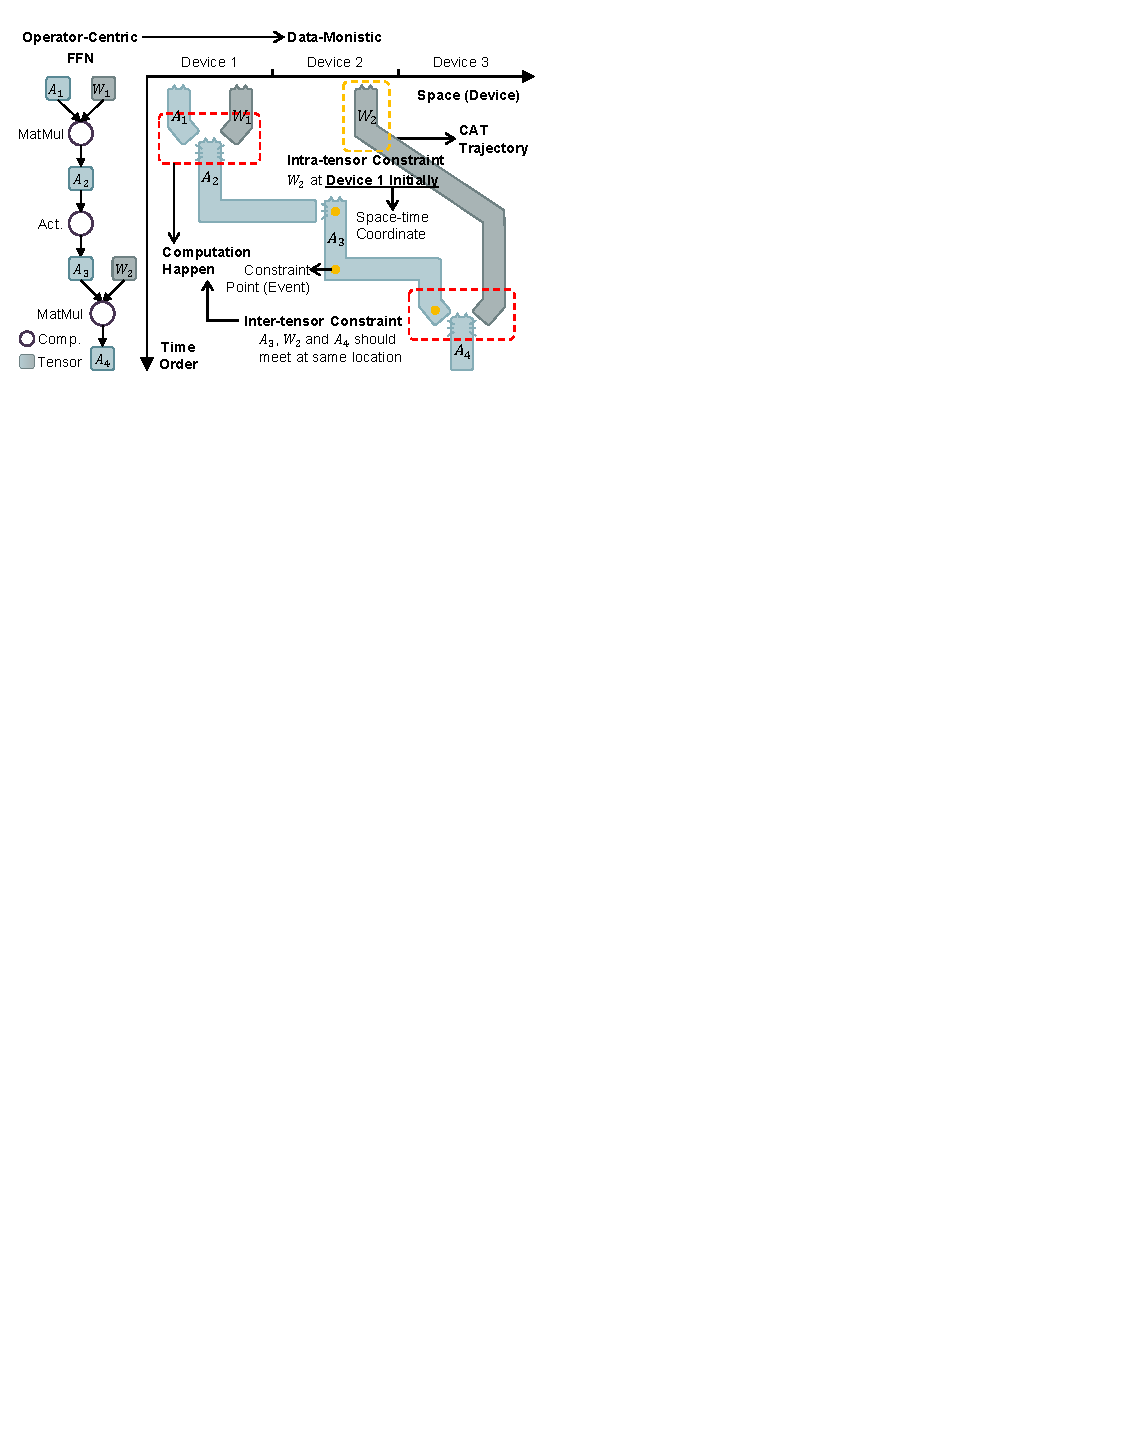
\includegraphics[width=1\linewidth]{figures/abstractions.pdf}
  \caption{Illustration of the data-monistic abstraction using an FFN layer in Transformer as an example. Each tensor is annotated with constraints explicitly with space-time coordinates. This abstraction enables fine-grained control over tensor partitioning, assignment, reduction, ordering, etc., supporting expressive strategies beyond operator-centric approaches.}
  \label{fig:abstractions}
\end{figure}

% Figure \ref{fig:primitives}(a) illustrates the difference between operator-centric and dataflow-centric perspectives. From the dataflow perspective, everything in the graph is represented by the \textit{flow} of data. Each tensor is not merely a static data block in memory, but a dynamic process. The \textit{head} of the arrow in Figure \ref{fig:primitives}(a) represents the beginning of tensor generation, and the \textit{tail} represents the completion of data generation. If the flow of \texttt{tensor1} and the flow of \texttt{tensor2} meet, the generation of \texttt{tensor3} will naturally be triggered. This dataflow perspective for describing NN workloads forms the foundation of our dataflow-centric primitives.


% 在之前的版本中，event 被放在 dependency 那一节介绍，但从逻辑上看，constraint point 应作为完整抽象描述的一部分，应该在此处介绍。
% 但这样做也有一些风险：
% 1. generation 和 consumption event 实际上就代表了计算。如果我们的抽象对其进行了精细描述，实际上等价于直接描述了计算的调度。我们的做法是用一种统一的方式来描述计算与数据流调度的超集。但在文章中不宜直接这样解释，否则会削弱“二元对立”的叙事，影响创新性的判断。
% 2. 末尾的 event 更准确地说代表数据释放，而非消费。
% 3. 在此处介绍 event 机制可能会增加文章前期的阅读难度，使 monistic 抽象显得复杂（而此处又无法展示这种复杂性带来的好处）。但总体来看，这一想法还是比较直接的。
% 4. 不同的 event 蕴含不同的“细节”。例如我们将 move 放在发送方而非接收方，那么如何确定发送目标？可通过下一个 event 的空间坐标判断。另外，约束向量并未描述设备间通信带宽和延迟等信息。
% 5. 关于 move 实现的一个潜在冲突：有时我们不希望指定两个约束点之间的具体路径（留给搜索算法探索），即两个约束点之间搜索算法可以插入新的约束点。这种“路径未知性”可能与 move 默认发送到下一个约束点所在设备的语义存在一定冲突。

A CAT is more than a static data block—it encapsulates both the data themselves and the dynamic trajectory of their generation, movement, and release. We use a series of \textbf{constraint points}, which form a \textbf{constraint vector}, to describe the space-time trajectory of a CAT. During implementation, these constraint points are realized as \textbf{events} that operate on the tensor. For instance, the first and last points in the constraint vector represent the CAT's generation and release events, respectively, and intermediate points typically signify movement events between devices. Figure \ref{fig:abstractions} demonstrates how a FFN layer is represented in the CAT abstraction. In this case, the trajectory of tensor $A_3$ is represented by the following constraint vector: $\mathbf{C}_{A_3} = [(\mathrm{Device}_2, t_1), (\mathrm{Device}_2, t_2), (\mathrm{Device}_3, t_3)]$. $\mathbf{C}_{A_3}$ also signifies its lifecycle: generated on Device 2 by consuming $A_2$, and sent to Device 3, where it is consumed to produce $A_4$.

This data-monistic abstraction is strictly more expressive than operator-centric approaches. Instead of treating data movement as an implicit side effect of operator scheduling, \name{} defines computation as a consequence of data colocation: an operator executes when its input tensors meet at the same space-time coordinate to generate output tensors in place. By describing the trajectory of data, we uniformly define the scheduling of computation, storage, and communication. This reversal allows \name{} to represent any operator-centric plan, plus a wider range of strategies that co-optimize computation and dataflow and manage complex data dependencies and movement.

\section{Primitives for Abstraction Manipulation}
\label{sec:primitives}
While directly manipulating each tensor's fine-grained constraints offers maximum flexibility, doing so for an entire parallelization plan is both tedious and error-prone. To simplify the construction of data-monistic abstractions, \name{} provides six high-level primitives and corresponding mechanisms. These primitives serve as auxiliary tools for building strategy spaces, connecting tensors and space-time coordinates through constraints to generate valid representations within \name{}. They can be categorized into three groups:

\textbf{Tensor distribution primitives}: This group, including \texttt{split}, \texttt{assign}, \texttt{copy}, and \texttt{reduce}, manages the spatial distribution of tensors. Together they define how data are partitioned, placed, and moved across devices.

\textbf{Dependency management primitives}: This group comprises \texttt{order} and \texttt{redirect}, which govern the logical temporal ordering of events. \texttt{order} enforces a specific dependency between events, whereas \texttt{redirect} transfers dependencies across tensors.

\textbf{Strategy-space delineation}: This mechanism declaratively defines and constrains the search space. For instance, a \texttt{domain} specifies the permissible range of values for a primitive's configuration (e.g., space-time coordinates), and \texttt{not} can explicitly exclude certain configurations.

In the following sections we demonstrate their usage through a walk-through example.

\subsection{Walkthrough Example}

FSDP is a data-parallelism strategy that reduces memory usage by sharding model parameters, gradients, and optimizer states across devices. During the forward pass, each device gathers the full parameters to perform computation, then discards them, retaining only its shard. In the backward pass, gradients are computed locally and immediately reduced and sharded to target devices via reduce-scatter, avoiding redundant storage. The sharding strategy consists of tiered levels of the ZeRO (Zero Redundancy Optimizer) framework~\cite{rajbhandari2020zero}: ZeRO-1 shards optimizer states, ZeRO-2 adds gradient sharding, and ZeRO-3 (the typical FSDP implementation) also shards parameters for maximum memory savings. At the operator level, these variants appear identical because data sharding does not involve operator partitioning; hence nnScaler cannot distinguish ZeRO-1 through ZeRO-3. Algorithm~\ref{alg:fsdp} shows how \name{}'s primitives can represent the core of ZeRO variants.

\begin{figure}[h]
  \centering
  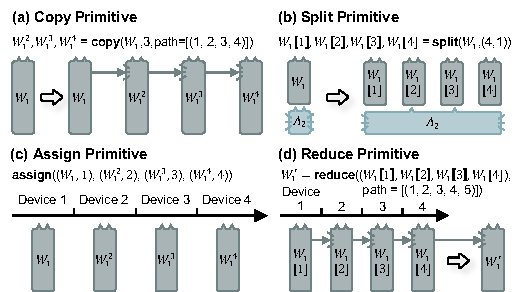
\includegraphics[width=1\linewidth]{figures/primitive_intro1.pdf}
  \caption{Illustration of data-centric primitives. (a) The \texttt{copy} primitive replicates tensors, enabling data replication across devices. (b) The \texttt{split} primitive partitions tensors, implicitly defining operator partitioning. (c) The \texttt{assign} primitive assigns tensors to devices, implicitly defining operator placement. (d) The \texttt{reduce} primitive manages data movement.}
    \label{fig:primitive_intro1}
\end{figure}

\begin{algorithm}[h]
\caption{Primitive program for vanilla DP and ZeRO-1 to 3. Assume the number of devices is 4.}
\label{alg:fsdp}
\begin{algorithmic}[1]
\STATE \# Vanilla DP: Replicate weights
\STATE $weight^2$, $weight^3$, $weight^4$ = \textbf{copy}($weight$, 3)
\STATE \textbf{assign}($weight^i$, $device_i$) \#$weight^1$ is $weight$
\STATE \# ZeRO-1: Add optimizer states sharding
\STATE $opt\_state[1$ to $4]$ = \textbf{split}($opt\_state$, 4)
\STATE \textbf{assign}($opt\_state[i]$, $device_i$)
\STATE \# ZeRO-2: Add gradients of weights sharding
\STATE $gradient[1$ to $4]$ = \textbf{split}($gradient$, 4)
\STATE \textbf{assign}($gradient[i]$, $device_i$)
\STATE \# ZeRO-3: Add weights sharding, no weight replication
\STATE $weight[1$ to $4]$ = \textbf{split}($weight$, 4)
\STATE \textbf{assign}($weight[i]$, $device_i$) 
\STATE $activation[1$ to $4]$ = \textbf{split}($activation$, 4, dim=BATCH)
\STATE \textbf{assign}($activation[i]$, $device_i$)
\end{algorithmic}
\end{algorithm}

% 关于Primitive的相关细节，若需展开，建议放在附录中说明：
% 1. 在abstraction部分已提到，CAT的轨迹由其constraint vector中的各事件点控制。因此，理论上原语应直接操作事件点而非tensor。文中以tensor为原语输入输出，实为语法糖：若tensor无时空约束，则视为静态数据块，原语操作直接作用于其本体；若tensor有时空约束，默认其位于同一device，原语操作亦无歧义。但若tensor轨迹跨设备，则split和copy的结果难以直观界定，若需定义可参考第2点。此外，reduce原语可理解为作用于tensor最后一个事件点的状态。
% 2. 关于约束的继承：若对已具复杂约束向量的tensor执行split或copy，合理做法是新生成的向量不继承原有约束向量。
% 3. 关于依赖的继承：split和copy所得tensor继承原输入的依赖关系。split原语会根据切分数据的具体部分判断应保留的约束，输出约束需自动化编译过程依据“最近的等价数据块”自动判定。
% 如何处理约束与依赖的继承机制，使CATFlow既不产生声明矛盾，也不影响自动化优化，是原语设计的一个挑战。
% 4. 原语的具体处理细节及默认行为，如split的切分向量维度设计、copy的路径指定、reduce的操作类型（如有）等。

Specifically, the following primitives are used:

\texttt{dst\_tensor=copy(src\_tensor, copy\_num, path)}: It copies the tensor specified by \texttt{src\_tensor} into \texttt{copy\_num} replicas. As illustrated in Figure \ref{fig:primitive_intro1}(a), the \texttt{path} parameter can specify the copy trajectory, e.g., $W_1^2$ is copied from $W_1$, $W_1^3$ is copied from $W_1^2$, etc.

\texttt{split\_tensors=split(tensor,split\_vector)}: It partitions a \texttt{tensor} into multiple sub-tensors (\texttt{split\_tensors}) according to \texttt{split\_vector} (Figure \ref{fig:primitive_intro1}(b)).

\texttt{assign(tensor, devices)}: It assigns \texttt{tensor} to a sequence of \texttt{devices}, specifying the spatial trajectory of the tensor across multiple locations (Figure \ref{fig:primitive_intro1}(c)).

During each layer's computation, it may be necessary to gather sharded weights or gradients from other devices; for example, in ZeRO-3, each device must collect all shards of the weight to compute the current layer's forward and backward passes. This process does not need to be explicitly represented in \name{}, as the backend compiler automatically infers and inserts such data-gathering based on data dependencies and constraints (see Section~\ref{sec:automated}). However, if required, the \texttt{reduce} primitive can be used to explicitly specify data gathering or reduction, as shown in Figure \ref{fig:primitive_intro1}(d).

\begin{figure*}[h]
  \centering
  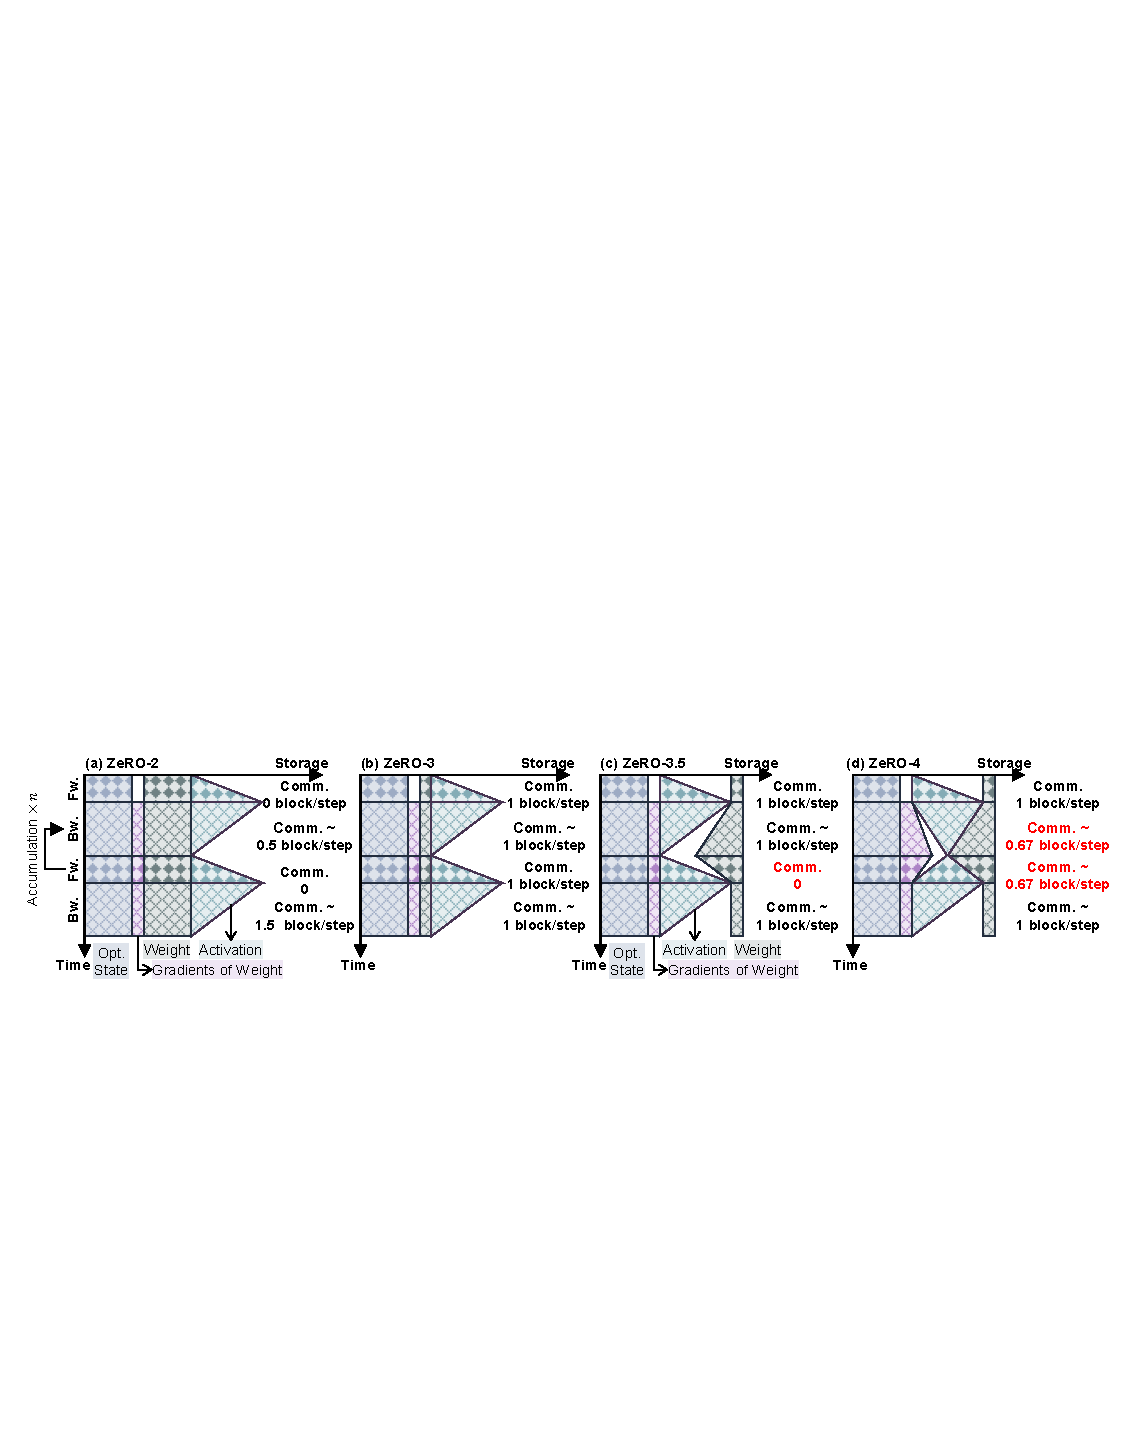
\includegraphics[width=1\linewidth]{figures/FSDP.pdf}
  \caption{Comparison of storage and communication volume during training for ZeRO-2, ZeRO-3 (existing methods), and ZeRO-3.5, ZeRO-4 (proposed by \name{}). Assuming each layer's forward computation takes one step and each device transmits one block of data per weight or gradient transfer. The duration of backward is twice as long as forward.}
    \label{fig:FSDP}
\end{figure*}

% 这段感觉应该放到附录，只放图展示结论即可
Figure \ref{fig:FSDP} illustrates the storage and communication patterns for ZeRO-2 and ZeRO-3. In ZeRO-2 (Figure \ref{fig:FSDP}(a)), each device holds the full model weights. Communication is concentrated at the batch boundaries: an `all-gather` for new weights before the forward pass and a `reduce-scatter` for gradients after the backward pass. During the dominant gradient-accumulation phase, only the gradient `reduce-scatter` is performed, leading to an average communication volume of 0.5 blocks/step. In contrast, ZeRO-3 (Figure \ref{fig:FSDP}(b)) shards weights for maximum memory savings, so each device holds only a weight partition. This requires an `all-gather` for every layer in both the forward and backward passes to assemble the full weights for computation. Consequently, the communication volume doubles to 1 block/step, becoming the performance bottleneck compared to ZeRO-2 (see Appendix for detailed computation). A strategy that achieves ZeRO-3's memory savings with ZeRO-2's communication efficiency would therefore be highly valuable.

\subsection{Dependency and Partial Temporal Order}
\label{sec:dependency}

We have demonstrated how CATFlow expresses strategies that are cumbersome to capture with operator-centric primitives. In this section, we further illustrate how the data-monistic approach articulates new strategies. As a case study, we augment ZeRO-3 with additional constraints that unlock an extra optimization opportunity: during the backward accumulation phase, activations are consumed progressively. Because their memory footprint usually dominates that of weights, the memory released by discarded activations can be immediately reused to host the incoming weight shards of the current layer. In the subsequent forward pass, weight shards are discarded layer-by-layer, and the freed space is reclaimed by newly generated activations, eliminating the all-gather communication of weights in the forward accumulation phase. We term this refined strategy ZeRO-3.5, shown in Figure~\ref{fig:FSDP}(c).

To implement this, we introduce a new primitive, \texttt{order}. As described in Section~\ref{sec:abstraction}, the event set of a CAT defines its space-time trajectory, and the ordering of events governs their temporal enactment. A typical use of event ordering is to enforce inter-CAT dependencies. Consider two CATs, $T_1$ and $T_2$, where $T_2$ can be created only after $T_1$ exists. This translates to the constraint that the start event of $T_2$ ($T_2\rightarrow\mathrm{start}$) cannot occur before the last event of $T_1$ ($T_1\rightarrow\mathrm{complete}$). We use $T\{i\}$ to reference the $i$-th event in the constraint vector of $T$ ($T\{0\}$ for $T\rightarrow\mathrm{start}$, $T\{-1\}$ for $T\rightarrow\mathrm{complete}$). While the system already preserves dependencies inherited from the original computational graph, the primitive \texttt{order(event$_1$, event$_2$)} explicitly injects additional ordering, ensuring that \texttt{event$_1$} occurs before \texttt{event$_2$}. In ZeRO-3.5, for instance, we use \texttt{order(}$A[i]^{\mathrm{microbatch}+1}\{-1\}$, $W^\mathrm{microbatch}\{-1\}$\texttt{)} to guarantee that weights gathered during the backward pass are retained until the corresponding activations of the next forward pass are completed. CATFlow further provides a syntactic-sugar primitive, \texttt{redirect(tensor$_1$, tensor$_2$, tensor$_3$)}, for complex dependency operations. If the original dependencies are $A_3 \to A_2 \to A_1$, applying \texttt{redirect(}$A_2, A_4, A_3$\texttt{)} creates $A_4$ from $A_2$ ($A_4$ also depends on $A_1$) and changes the dependency of $A_3$ from $A_2$ to $A_4$. The redirect primitive can be used to achieve advanced strategies such as recomputation and dataflow reconfiguration (details in Appendix).

We further proposes ZeRO-4 that selectively delays reduce-scatter on weight gradients with \texttt{order($A[j]^{\mathrm{microbatch}+1}\{-1\}$}, $gradient^{\mathrm{microbatch}+1}[j]\{0\}$\texttt{)}. This essentially allows the gradients of certain layers to remain on the local device during the backward pass. The reduce-scatter is postponed until forward activations have accumulated and consumed more memory. This strategy enables more balanced backward–forward communication by exploiting variations in available memory capacity. In the example shown in Figure~\ref{fig:FSDP}(d), we choose $j$ to be multiples of three, that is, retaining one layer's gradient for every three layers. In practice, the choice of $j$ can be determined according to the communication-memory trade-off.

\subsection{Strategy Space Delineation}
\label{sec:delineation}

As the preceding discussion shows, \name{}'s primitives are fundamentally a series of declarative constraints. By default, \name{} posits that the initial strategy space—before any primitives are written—is the universal set of all valid parallelization plans for a given computation graph and hardware system, constrained only by inherent data dependencies. In contrast to operator-centric frameworks, which imperatively construct a strategy from a null state, applying a primitive in \name{} is a subtractive process. Each primitive declaratively refines the strategy space by imposing an additional constraint, thereby narrowing the universe of valid plans. This approach can yield unforeseen strategies that are not explicitly encoded by the user. The resulting strategy space is then passed to a search algorithm (Section \ref{sec:search}) and a compilation process (Section \ref{sec:automated}) to materialize a concrete, high-performance plan. This design philosophy necessitates that \name{} provide users with effective mechanisms to guide the delineation of the strategy space and to express strategic preferences.

\begin{figure}[h]
  \centering
  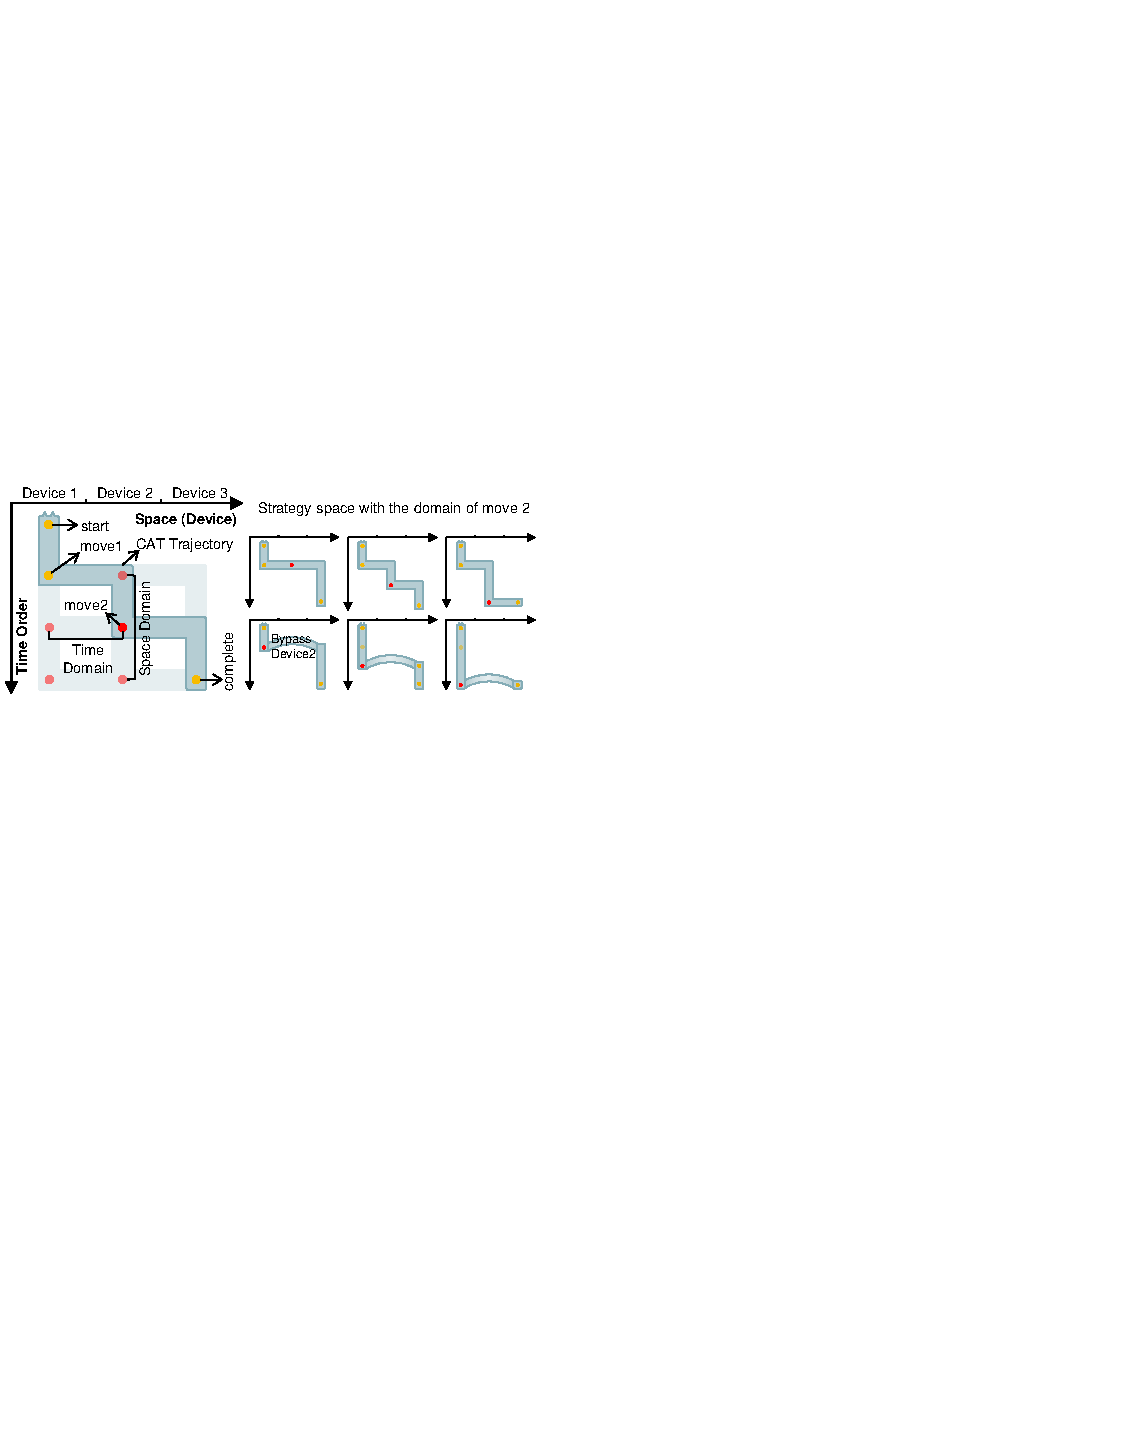
\includegraphics[width=1\linewidth]{figures/primitive_intro2.pdf}
  \caption{The spatial and temporal domain of \texttt{move2} yields a strategy space encompassing six feasible CAT trajectories.}
  \label{fig:primitive_intro2}
\end{figure}

A primary mechanism is the \textbf{\texttt{domain}}. A domain represents a discrete, iterable set of valid candidates for a given parameter, such as a device location or a time step. For example, a user can define \texttt{d = Domain(Device1, Device2, Device3)} and then apply the constraint \texttt{assign(tensor/event, d)}. This declaration does not specify which of the three devices the tensor or event should be assigned to; rather, it constrains the search space by asserting that the assignment must be one of the devices within domain \texttt{d}. As illustrated by the shaded region in Figure \ref{fig:primitive_intro2}, imposing event \texttt{move2} in the spatial domain \texttt{(Device1, Device2)} and the temporal domain \texttt{(move1, complete)} can yield six possible CAT trajectories in this space. The \textbf{\texttt{not}} declaration provides a subtractive mechanism for space delineation. It allows users to explicitly forbid certain configurations by combining it with the aforementioned primitives and \texttt{domain}. For instance, \texttt{not(assign(tensor, d))} means the tensor should not be mapped to domain \texttt{d}.

% (The temporal domain is a partial-order domain defined by Order Ideals and Order Filters; we do not delve deeper into this topic in the paper.)

We further introduce \textbf{\texttt{symmetry}}, a mechanism that binds a set of CATs to perform uniform actions during search, thereby reducing search dimensionality and avoiding highly irregular outcomes. Let $S=\{\text{CAT}_1,\ldots,\text{CAT}_k\}$ be a symmetry group and $I=\{1,\ldots,k\}$ its index set. A symmetry declaration is written as \texttt{symmetry($S$, ${i\in I \to \mu(i))}$}, where $\mu(i)$ is a parameterized step schema (e.g., \texttt{assign($\text{CAT}_i$, $\text{device}_{\mu(i)}$)}, \texttt{order($\text{CAT}_i, W[\mu(i)]$)}). During search, the grouped CATs are treated as a single object for search move selection and evaluation: the algorithm either applies the candidate move to all members simultaneously or to none, and feasibility is jointly assessed across all member constraints. Symmetry-binding thus biases the search toward coherent patterns while still admitting per-CAT variation via indexed parameters.
We present more examples of \name{}'s primitives in Appendix.

\section{Constraint-Based Potential Descent Search}
\label{sec:search}

% 可以考虑加入问题的形式化

The fine-grained control over tensor trajectories and the subtractive method of carving the strategy space can result in a potentially larger search space. While this is advantageous for including emergent strategies and creating a more connected, higher-resolution landscape for heuristic search, it also inherently increases the search complexity. Therefore, a biased reduction of the space at the primitive stage is not only necessary but also plays a crucial role in guiding the subsequent search phase. We do not claim that our method can automatically find an optimal strategy from the universal set of all possibilities. Moreover, a rigorous mathematical analysis of the properties of this data-monistic search space, for instance, whether this unified abstraction enhances the topology smoothness and continuity, is beyond the scope of this paper. Instead, this section presents a feasible search algorithm from the CAT perspective. The efficacy of this algorithm in discovering novel strategies will then be demonstrated empirically in Section \ref{sec:exp}.

The search algorithm is inspired by potential-field methods. It reframes the combinatorial-optimization problem as the search for a minimum-energy state in a potential field. At its core, the algorithm assigns a potential function to every CAT; each CAT then greedily migrates or transforms to a state that lowers its own potential. A simple illustrative example: suppose CAT1 currently resides on device 1. If we define the potential of CAT1 as the memory already occupied on that device, CAT1 will tend to migrate to a device with lower occupancy (more free memory). Repeating this greedy minimization for every CAT yields a reasonably balanced memory distribution, e.g., Bpipe~\cite{kim2023bpipe}.

% 势能是分层次的，event点处的势能，CAT的整体的势能。核心的点就是是CAT尽量少占用资源。
Real scenarios are far more complicated. A strategy comprises many CATs, and each CAT contains a constraint vector composed of multiple events. Although each event can be scheduled independently, intricate dependencies may exist among events. Our search algorithm therefore employs a two-level potential definition, with each level paired with its own set of searchable actions (the next search move).

Level-1 potential is attached to individual events. In a deterministic plan, an event’s space–time coordinate is fixed; its potential is therefore quantified by the resource pressure of the underlying hardware at that coordinate. With respect to the optimization objective we track three resources—compute, memory, and communication—and define the event-level potential as the event’s demand minus the residual capacity of the device. The search actions an event can perform are either reordering itself along the time dimension or migrating to another device.

Level-2 potential is associated with an individual CAT. It comprises two main components. The first, the intrinsic potential, is the aggregation of the level-1 potentials of all event points within the CAT’s own constraint vector $C=(C_1,C_2,\ldots ,C_n)$, representing the direct resource cost of its current trajectory. However, a locally beneficial move for one CAT may induce significant cost increases in other interdependent CATs. To mitigate this, we introduce a second, corrective term. This term subtracts the aggregate potential of all event points belonging to other CATs that are coupled with the current CAT through inter-CAT constraints. This design endows the level-2 potential with a degree of global awareness without simulating the overall performance at every possible action step. The potential for a CAT is thus formulated as

\[
P(\text{CAT})=\sum_{i=1}^{n}P(C_i)-\sum_{\text{CAT}'\in\mathcal{A}(\text{CAT})}\sum_{j=1}^{m}P(C'_j)
\]
where $\sum P(C_i)$ is the CAT's intrinsic potential, $\mathcal{A}(\text{CAT})$ is the set of all CATs associated with the current CAT via inter-CAT constraints.

Search actions for a CAT includes three categories. 1. modifying a single event within the CAT's constraint vector. To manage the complexity arising from intricate inter-event dependencies, we restrict these moves to atomic, single-event changes. The optimal move for each event is determined independently by identifying the steepest descent direction of its Level-1 potential. 2. altering the dimensionality of the constraint vector itself. This is achieved through two primary approach: the deletion of an existing event, or the insertion of a new move event between two consecutive points in the tensor's trajectory. 3. appling macro-level scheduling operations to the entire CAT, including split, copy, or reduce. The available transformations are generated by enumerating the set of permissible high-level policies defined by the primitives and domains. The union of all three categories constitutes the complete set of feasible candidates for the CAT's next step in the search process.

\begin{algorithm}[h!]
\caption{Two-Level Potential-Guided Greedy Search}
\label{alg:structured_search}
\begin{algorithmic}[1]
\STATE $S \gets S_{initial}$
\FOR{$i = 1$ to $max\_iterations$}
  \STATE $best\_cat \gets \text{None}$; $best\_move \gets \text{None}$; $best\_\Delta \gets 0$
  \FOR{each CAT $T$ in $S$}
    \STATE $P_T \gets \text{CalculateCatPotential}(T, S)$
    \STATE $C_{event} \gets \text{GenerateEventCandidates}(T, S)$
    \STATE $C_{vector} \gets \text{GenerateVectorCandidates}(T, S)$
    \STATE $C_{macro} \gets \text{GenerateMacroCandidates}(T, S)$
    \STATE $M_T \gets C_{event} \cup C_{vector} \cup C_{macro}$
    \STATE $\begin{aligned}
    m_T^{\star} &\gets \operatorname*{argmax}\limits_{m \in M_T} \left(P_T - \text{CalculateCatPotential}(T, \\
    &\text{ApplyCatMove}(S, T, m))\right)
    \end{aligned}$
    \STATE $\begin{aligned}
    \Delta_T &\gets P_T - \text{CalculateCatPotential}(T, \\
    &\text{ApplyCatMove}(S, T, m_T^{\star}))
    \end{aligned}$
    \IF{$\Delta_T > best\_\Delta$}
      \STATE $best\_cat \gets T$; $best\_move \gets m_T^{\star}$; $best\_\Delta \gets \Delta_T$
    \ENDIF
  \ENDFOR
  \IF{$best\_\Delta \le 0$}
    \STATE \textbf{break}
  \ENDIF
  \STATE $S \gets \text{ApplyCatMove}(S, best\_cat, best\_move)$
\ENDFOR
\STATE \textbf{return} $S$
\end{algorithmic}
\end{algorithm}

The search procedure is a greedy, iterative process that begins with an initial strategy sampled from the space defined by our primitives. At each iteration, the algorithm seeks to make the most impactful local improvement. To do this, it first evaluates the current potential of every CAT. For each CAT, it then explores all of its next-step candidates to find its locally optimal step, which is the move that maximally reduces its own potential. Once the optimal step and its corresponding potential reduction have been identified for all CATs, the algorithm performs a global selection. It identifies the optimal CAT: the one whose optimal step promises the largest potential drop. The algorithm commits to this single best move, executing the optimal step for the optimal CAT to update the parallelization plan. This cycle repeats until convergence is achieved or another termination criterion is satisfied.

Algorithm~\ref{alg:structured_search} instantiates the potential-field view described above. Each iteration evaluates the current CAT potential, enumerates event-, vector-, and macro-level candidates for every CAT, selects the locally optimal move that maximally reduces its own potential, and then performs a global selection to commit the single move with the largest potential drop.

\texttt{CalculateCatPotential} calculates level-2 potentials. \texttt{GenerateEventCandidates} restricts changes to single-event reordering or migration following the steepest-descent direction. \texttt{GenerateVectorCandidates} inserts or deletes move events. \texttt{GenerateMacroCandidates} applies high-level transformations such as split, copy, or reduce. Algorithm~\ref{alg:generate_event_candidates} shows the detailed routine of \texttt{GenerateEventCandidates}. Device candidates are enumerated from the spatial adjacents; time candidates are the immediately preceding or succeeding order positions. For each event, the routine enumerates the Cartesian product of adjacent devices and times, evaluates the event potential on each spatiotemporal pair, and selects the steepest-descent pair while preserving all constraints.

\begin{algorithm}[h]
\caption{GenerateEventCandidates$(T, S)$}
\label{alg:generate_event_candidates}
\begin{algorithmic}[1]
\STATE $C \gets \emptyset$
\FOR{each event $e$ in the constraint vector of $T$}
  \STATE $\mathcal{D}_e \gets \text{AdjacentDevices}(e, S)$
  \STATE $\mathcal{T}_e \gets \text{AdjacentTimes}(e, S)$
  \STATE $m^{st}_e \gets \operatorname*{argmin}\limits_{(d,t) \in \mathcal{D}_e \times \mathcal{T}_e}(\text{EventPotential}(e, d, t, S))$
  \IF{$\text{DecreasePotential}(e, m^{st}_e, S)$ \textbf{and} $\text{Feasible}(e, m^{st}_e, S)$}
    \STATE $C \gets C \cup \{\text{MakeMove}(e, m^{st}_e)\}$
  \ENDIF
\ENDFOR
\STATE \textbf{return} $C$
\end{algorithmic}
\end{algorithm}

\section{Implementation}
\label{sec:automated}

% because it builds on the explicit scheduling of data trajectories
The data-monistic abstraction of \name{} represents a paradigm shift from existing operator-centric distributed-training frameworks such as DeepSpeed or Megatron, whose core architectures (IR, schedulers, runtimes) are deeply integrated to schedule operators. Retrofitting \name{} into these frameworks is extremely difficult. Moreover, this architectural mismatch culminates in an incompatible runtime. While existing systems are designed to execute a pre-compiled sequence of computational kernels and communication collectives, it remains an open research topic how to dynamically interpret a data-centric schedule to generate efficient low-level CUDA kernels on the fly. Therefore, \name{} is not implemented as an end-to-end system but rather serves as a strategy-exploration framework. It discovers parallelization plans that are then manually implemented in CUDA kernels or existing frameworks for high-performance execution.

\begin{figure}[h]
  \centering
  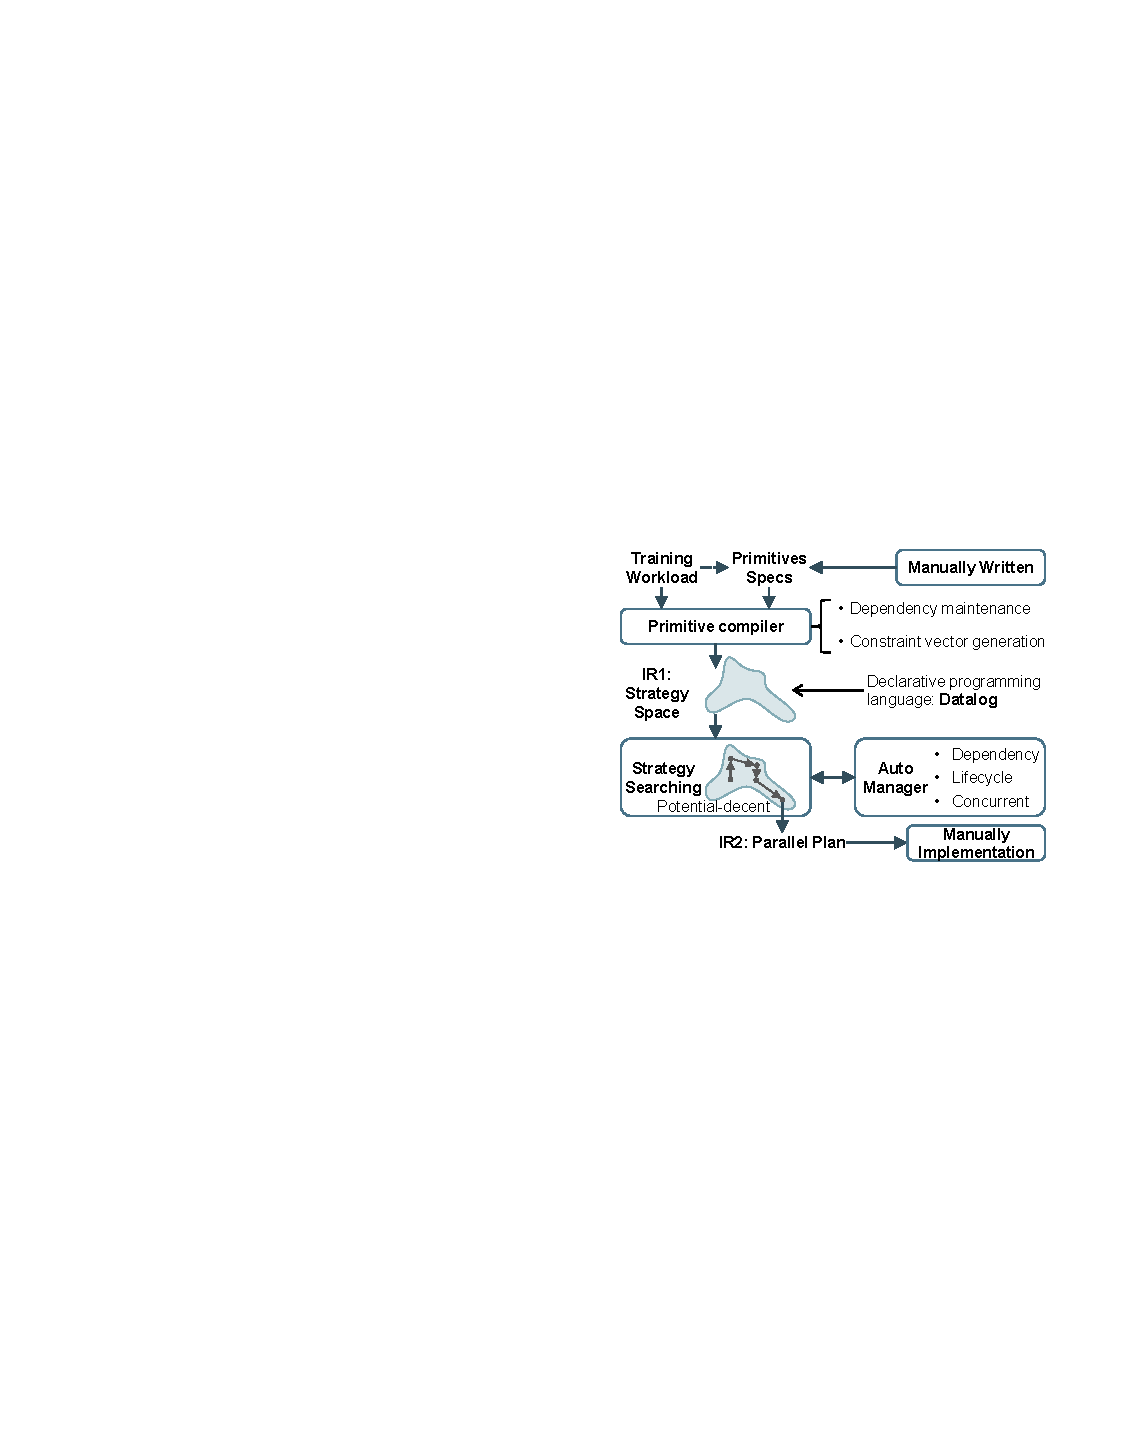
\includegraphics[width=0.7\linewidth]{figures/implementation.pdf}
  \caption{Implementation stack of \name{}.}
    \label{fig:implementation}
\end{figure}

Beyond these difficulties, our implementation focuses on two aspects: (1) Primitive Compilation \& Strategy-Space IR (IR1) — the design of the primitive interface in high-level languages and its compilation into a constraint-declarative strategy-space intermediate representation; (2) Search \& Plan Synthesis (IR2) — the search procedure over IR1, augmented with automatic management rules, that yields a concrete parallelization plan. The basic implementation stack of \name{} is shown in Figure \ref{fig:implementation}.

\subsection{Primitive Compilation}
\label{sec:primitive_compilation}

We implement our primitives in Python, with the tensor identifier coming from the training workload. Each primitive invocation is translated into a set of declarative constraints in Datalog; the strategy-space IR1 itself is represented in Datalog to enable constraint normalization. Datalog is a declarative logic-programming language based on Horn clauses. We adopt Datalog because it is a universal language for constraint specification and integrates cleanly with Python. IR1 captures, for every CAT, its constraint vector (event set), the spatial and temporal domains of each event, inter-CAT couplings (including dependencies and symmetries), and resource constraints. The primitive compiler is responsible for maintaining IR invariants while applying the transformations specified by the primitives. The most critical invariant is dependency preservation: if a CAT $B$ depends on CAT $A$, and a primitive transforms $A$ (e.g., \texttt{split}, \texttt{copy}) into derived CATs or data blocks, the compiler rewrites $B$'s dependencies to target the transformed set that semantically replaces $A$.

To ensure correct dependency rewriting, every data block in the training workload is assigned a globally unique identifier. Derived blocks carry provenance metadata of the form $(\text{origin\_id}, \text{range})$, which records their position within the original tensor. When primitives create new blocks, the compiler compares the positional intervals of producer and consumer blocks: overlaps introduce new dependencies, whereas disjoint intervals allow the dependency to be removed. nnScaler employs a similar mechanism; we therefore adopt its intersection-based matching approach. For \texttt{copy} primitives that may introduce redundant dependencies, the compiler retains the redundancy and defers selection of the optimal dependency to the plan-synthesis stage.

Temporal constraints are encoded through a Lamport logical time system. Each event is assigned a unique timestamp; however, when an event possesses a temporal domain, its timestamp is superseded by a partial-order domain induced by other events. For instance, if event $e$ must occur after both $e_1$ and $e_2$ and before $e_3$, and $e_1$ and $e_2$ are unordered (means concurrent in the Lamport system), the constraint is represented as $(\{e_1,e_2\},e_3)$.

Each CAT is associated with a constraint vector for events. The compiler designates the first point of the vector as the generation event of the CAT and the final point as its release event. Intermediate points are interpreted as \emph{move} events, indicating a change in the CAT's spatial location. If such an event does not alter the spatial coordinates, the compiler eliminates it and rewrites any dependencies that involved the removed event to its nearby event.

\subsection{Plan Synthesis}
\label{sec:plan_synthesis}

The strategy search is performed via the potential-descent algorithm described in Section~\ref{sec:search}. At every search iteration, a concrete strategy (IR2) within the space is synthesized. To ensure unambiguous interpretation, we adopt a set of default management rules that complement the explicitly declared constraints.

\begin{figure}[h]
  \centering
  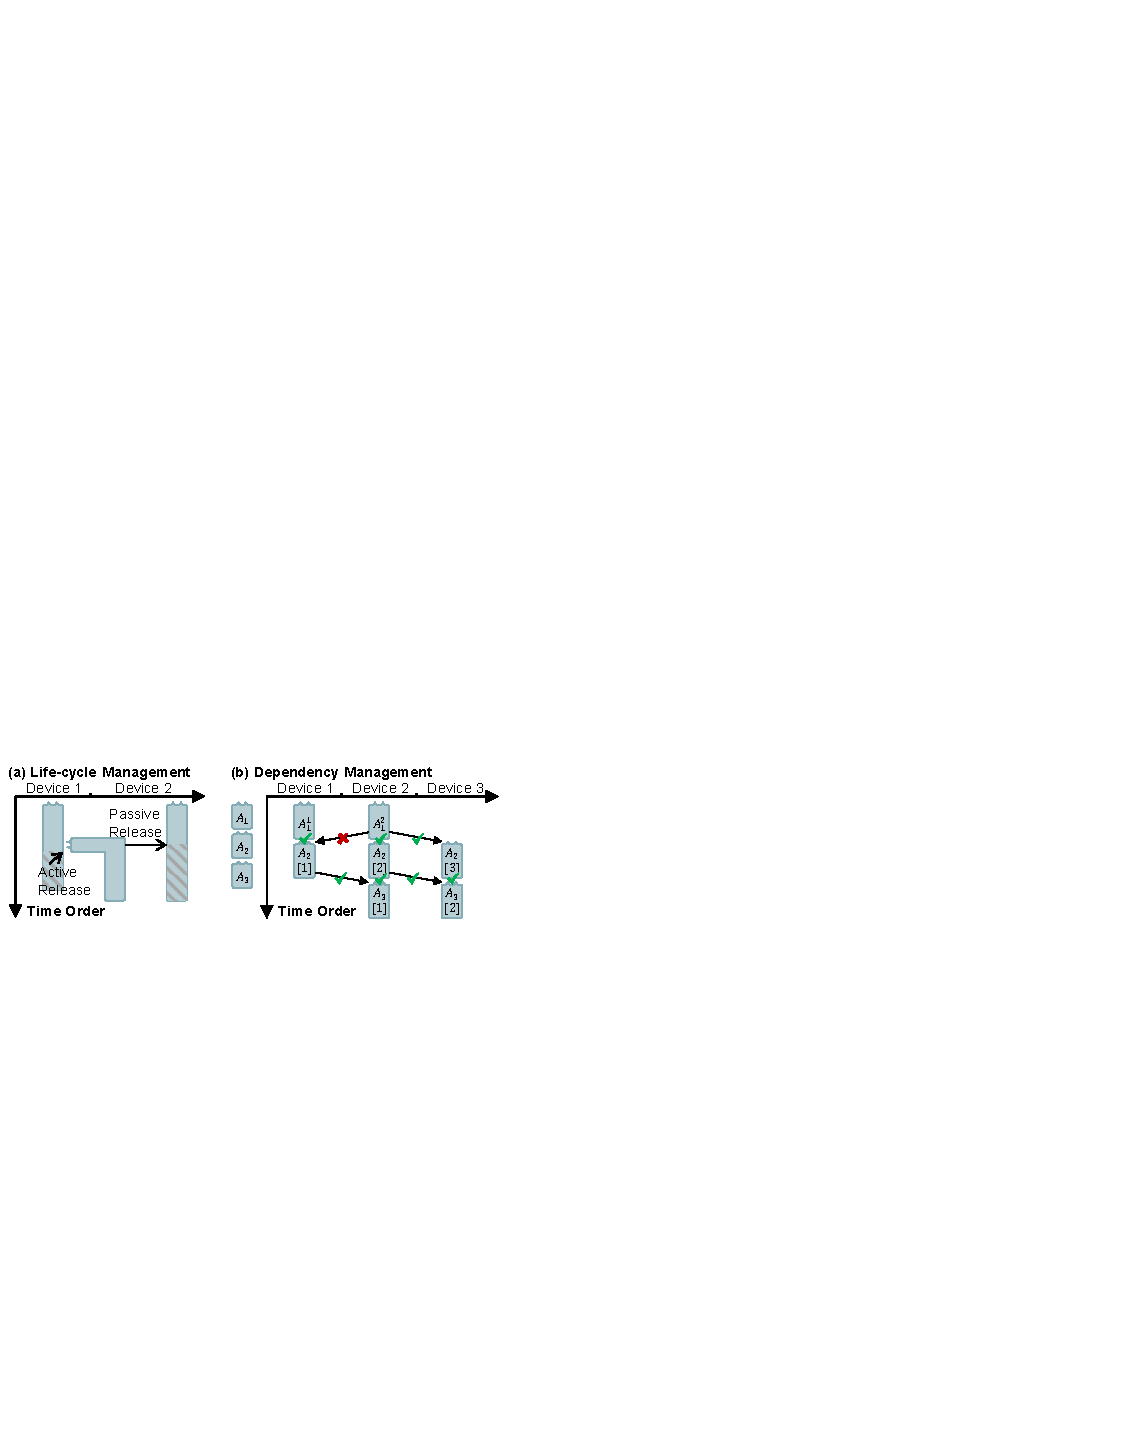
\includegraphics[width=0.95\linewidth]{figures/management.pdf}
  \caption{Illustration of automatic lifecycle and dependency management.}
    \label{fig:management}
\end{figure}

\textbf{Lifecycle Management:} The lifecycle ensures that each tensor is properly released after its usage. It implements two rules: (1) \emph{active release}: a CAT is freed immediately once no subsequent event depends on it; (2) \emph{passive release}: a CAT may remain in memory even when unreferenced, but is evicted when memory pressure exceeds a predefined threshold (Figure~\ref{fig:management}(a)). These rules may steer the search algorithm toward different strategies due to their different influences on potential evaluation.

\textbf{Dependency Management:} A CAT may depend on other CATs whose data are scattered across multiple devices. The \texttt{copy} primitive can also render the dependencies recorded in IR1 redundant. The dependency manager therefore materializes a CAT's complete forward dependencies on demand. It first enumerates every required predecessor, then fetches them in ascending order of estimated acquisition cost until all dependencies are satisfied. For instance, if CAT $A$ on device-1 needs CAT $B$ and $B$ exists on both device-1 and device-2, $A$ prefers to consume the local replica, eliminating inter-device transfer. Figure~\ref{fig:management}(b) illustrates some cases involving \texttt{split} and \texttt{copy}.

\textbf{Concurrent Management:} Events whose temporal order is unspecified may be executed concurrently. We currently model the most common case: overlapping computation with communication. Other concurrent events are temporarily excluded because it is hard to find universal rules for them. For example, multiple move events will still be executed in a default order even when no order constraint is imposed.

\section{Evaluation}
\label{sec:exp}

\subsection{Experiment Setup}
\label{sec:exp_setting}

We structure our evaluation in three phases to assess the efficiency of \name{}'s generated strategies and its search procedure. First, we compare ZeRO-2 and ZeRO-3~\cite{rajbhandari2020zero} to ZeRO-3.5 and ZeRO-4 across different LLMs and hardware configurations, focusing on training throughput and peak memory usage. Second, we demonstrate \name{}'s search capability: starting from a ZeRO-3 initialization, we trace how the potential distribution evolves under potential descent toward ZeRO-3.5 and ZeRO-4. Finally, through comprehensive experiments, we identify seven scheduling optimization directions suggested by potential descent under different hardware resource configurations. By combining several of these directions, \name{} discovers and implements a novel offloading strategy that shows improved performance relative to standard offloading strategies. 

\name{}'s expressiveness and search capability enable exploration of coordinated, cross-resource trade-offs, including leveraging partial redundancy in one resource to alleviate bottlenecks in another. Accordingly, \name{} focuses on improving utilization with tight resource budgets on small clusters, rather than on scaling under ever-increasing resources. The objective is to democratize the training of LLMs for small companies and laboratories~\cite{sun2025mepipe}. Consistent with this objective, we perform the following experiments on clusters with 8 GPUs.

\textbf{Models and Hardware.} We evaluate strategies on 8B, 14B, and 32B models (Qwen3 family~\cite{yang2025qwen3}, Table~\ref{tab:qwen3_params}). For hardware, we use four configurations: NVIDIA A100-NVLink, H20-NVLink, H800-PCIe, and A100-PCIe. Compute capacity: H800 > A100 > H20; interconnect bandwidth: H20-NVLink (900 GB/s) > A100-NVLink (400 GB/s) > H800-PCIe (128 GB/s) > A100-PCIe (64 GB/s); memory capacity: H20-NVLink (96 GB) > H800-PCIe = A100-NVLink (80 GB) > A100-PCIe (40 GB). Intel Xeon Platinum 8558 CPU (80/96/128/160 cores) is adopted for offload-related experiments.

\begin{table}[h]
  \centering
  \caption{Qwen3 series model configurations}
  \vspace{-0.5em}
  \label{tab:qwen3_params}
  \begin{tabular}{ccccc}
    \toprule
    Model & Params & Layers & Hidden & Heads (Q/KV) \\
    \midrule
    Qwen3  & 8B  & 36 & 4096  & 32/8 \\
    Qwen3 & 14B & 40 & 5120 & 40/8 \\
    Qwen3 & 32B & 64 & 5120 & 64/8 \\
    \bottomrule
  \end{tabular}
  \vspace{-1em}
\end{table}

\textbf{Implementation and Configuration.} For potential evaluation during search, we use a behavioral simulator that estimates compute, storage, and bandwidth usage, calibrated against an A100-based cluster. On real systems, we extend DeepSpeed's ZeRO-3 implementation with ZeRO-3.5/4 and offload-related strategies, and we unify other settings (e.g., reduce/prefetch bucket sizes, maximum live parameters) to ensure fair comparisons. We replace the default Linear layer with a memory-efficient Linear to mitigate potential memory leakage in DeepSpeed.\footnote{\url{https://github.com/deepspeedai/DeepSpeed/issues/3378}.} We use FP16-FP32 mixed-precision training. Detailed configurations are reported with the results. 

% For each strategy, we sweep batch sizes and sequence lengths;

\begin{figure}[h]
  \centering
  \begin{subfigure}{0.7\linewidth}
    \centering
    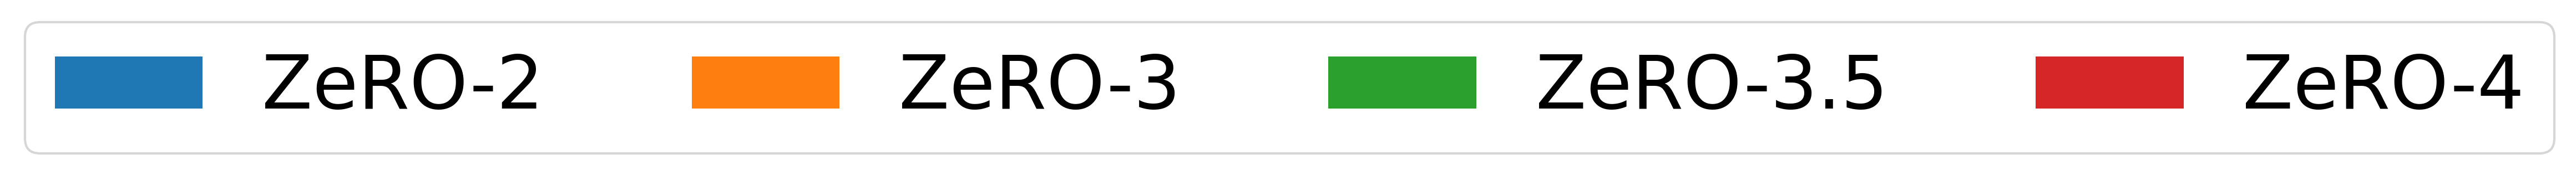
\includegraphics[width=\linewidth]{figures/legend.png}
    \vspace{-1.4em}
  \end{subfigure}
  \begin{subfigure}{0.49\linewidth}
    \centering
    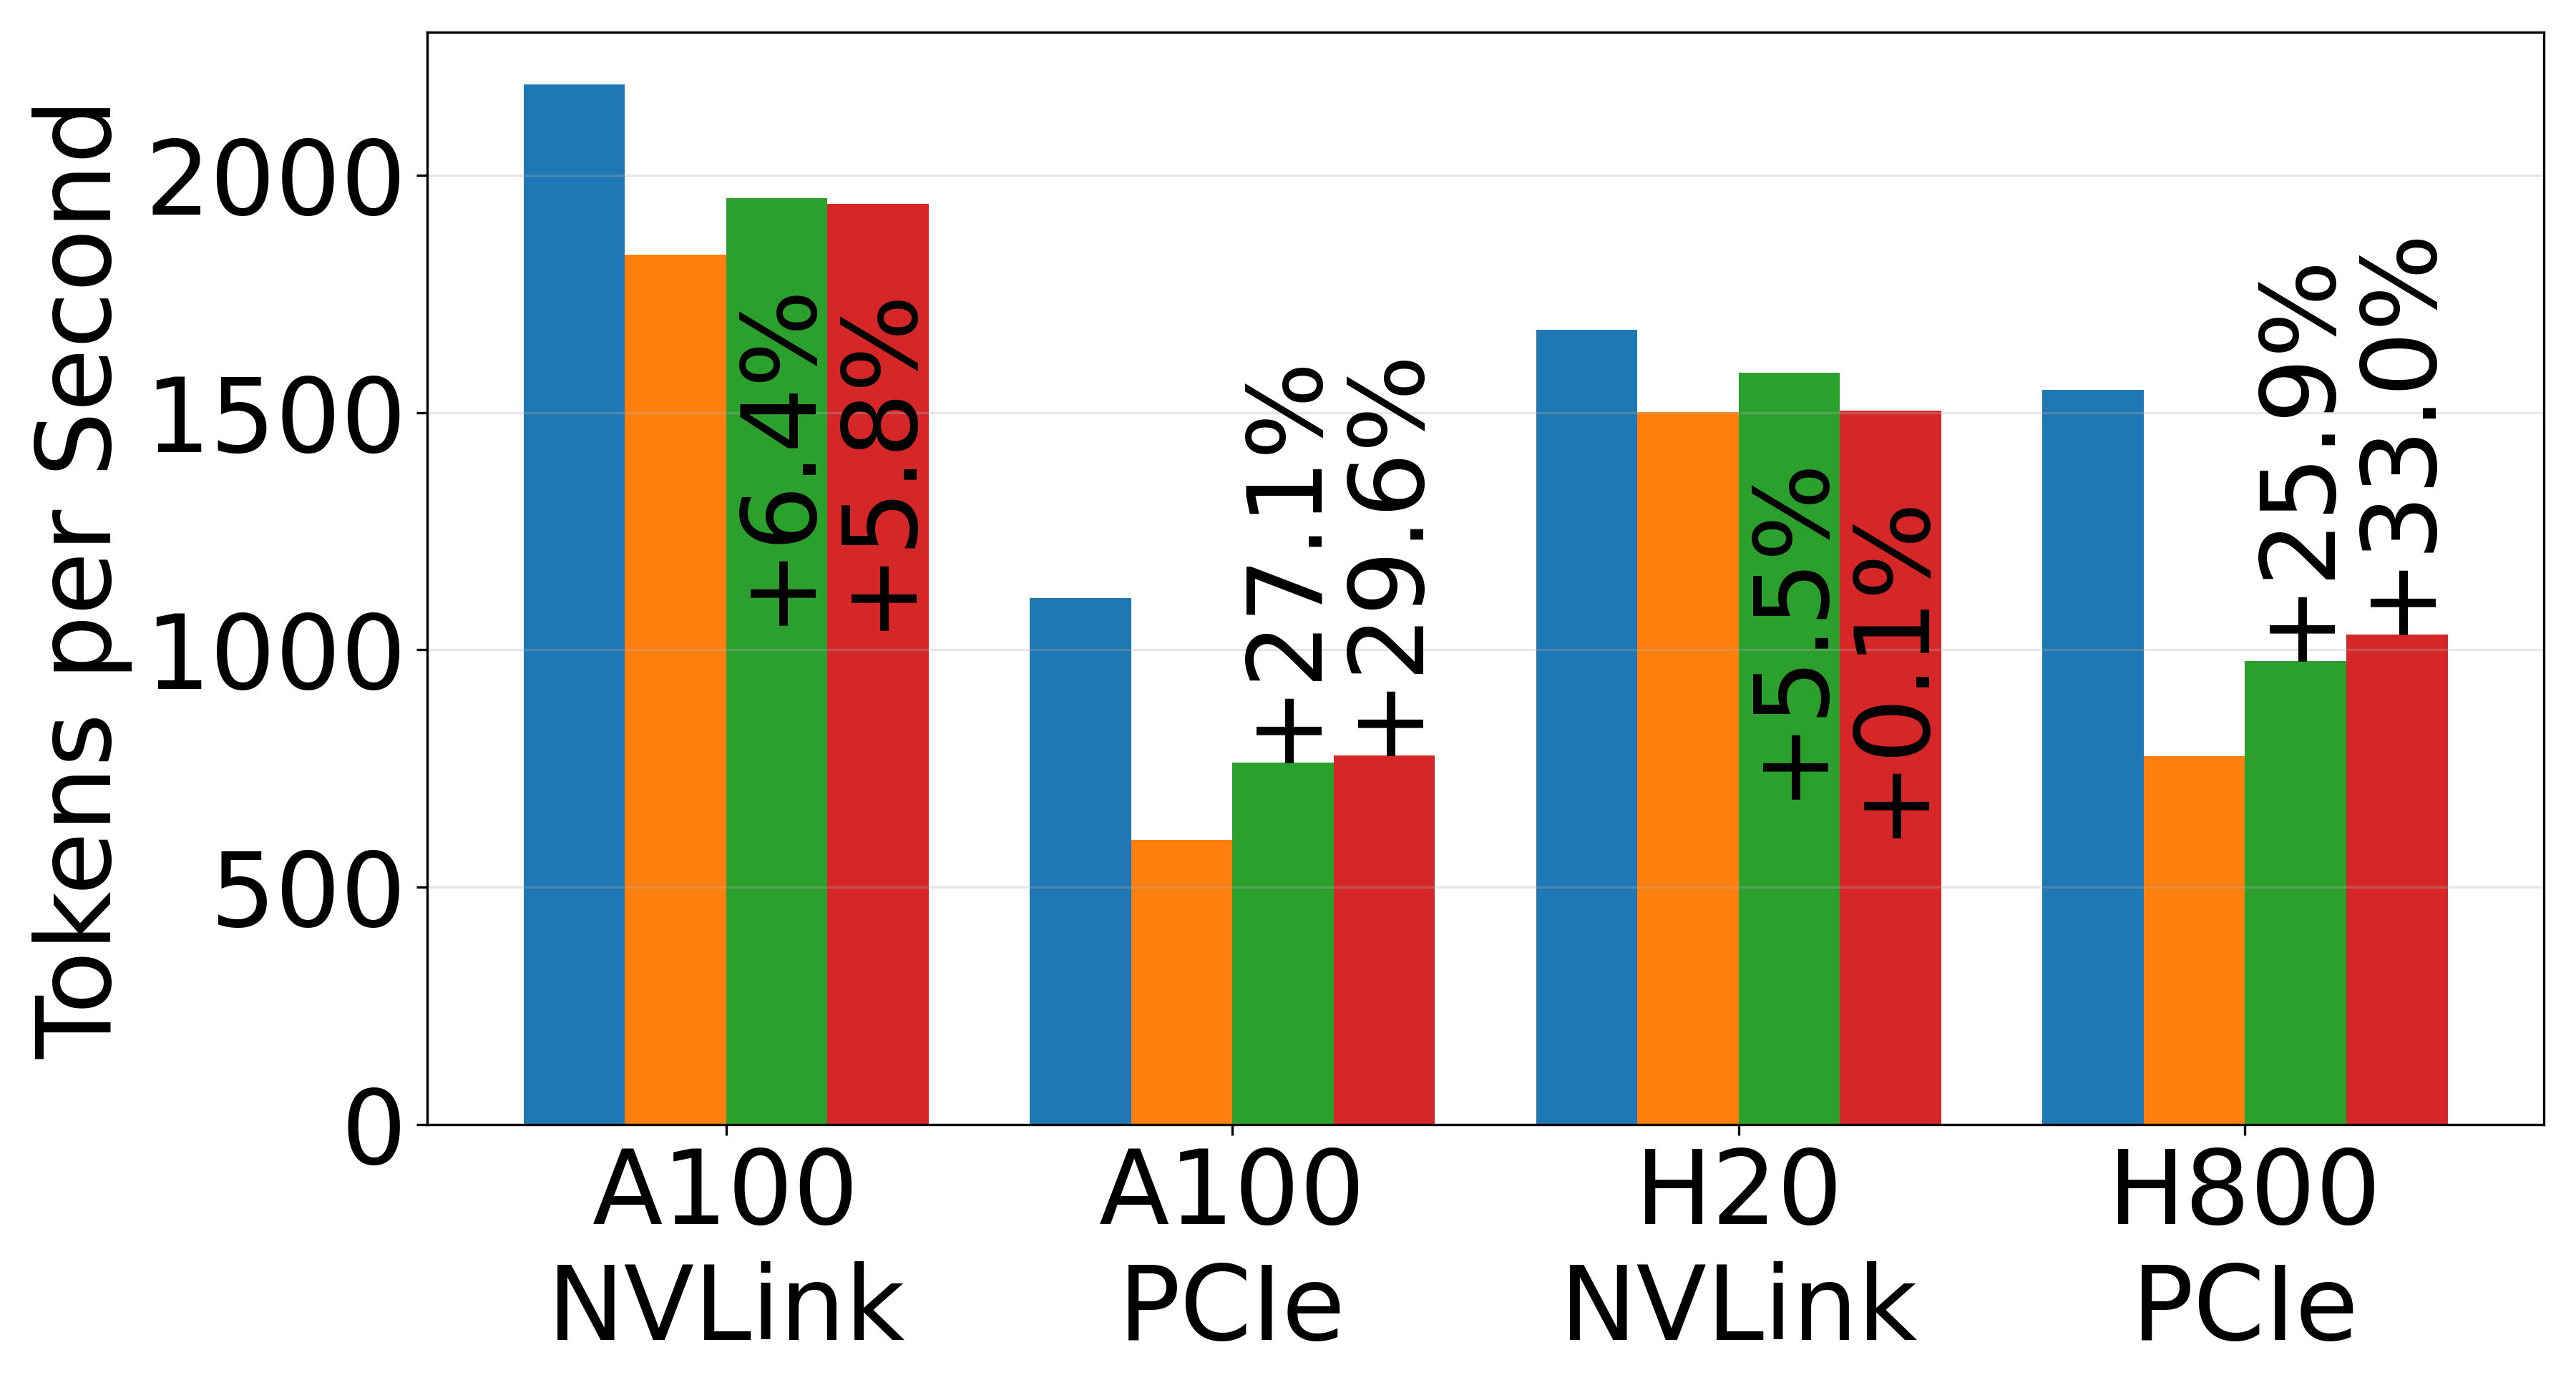
\includegraphics[width=\linewidth]{figures/hardware_comparison_b1_s1536_tokens_per_sec_qwen3-8b.png}
    \vspace{-1.5em}
    \caption{8B|B=128|S=1.5K}
  \end{subfigure}
  \begin{subfigure}{0.49\linewidth}
    \centering
    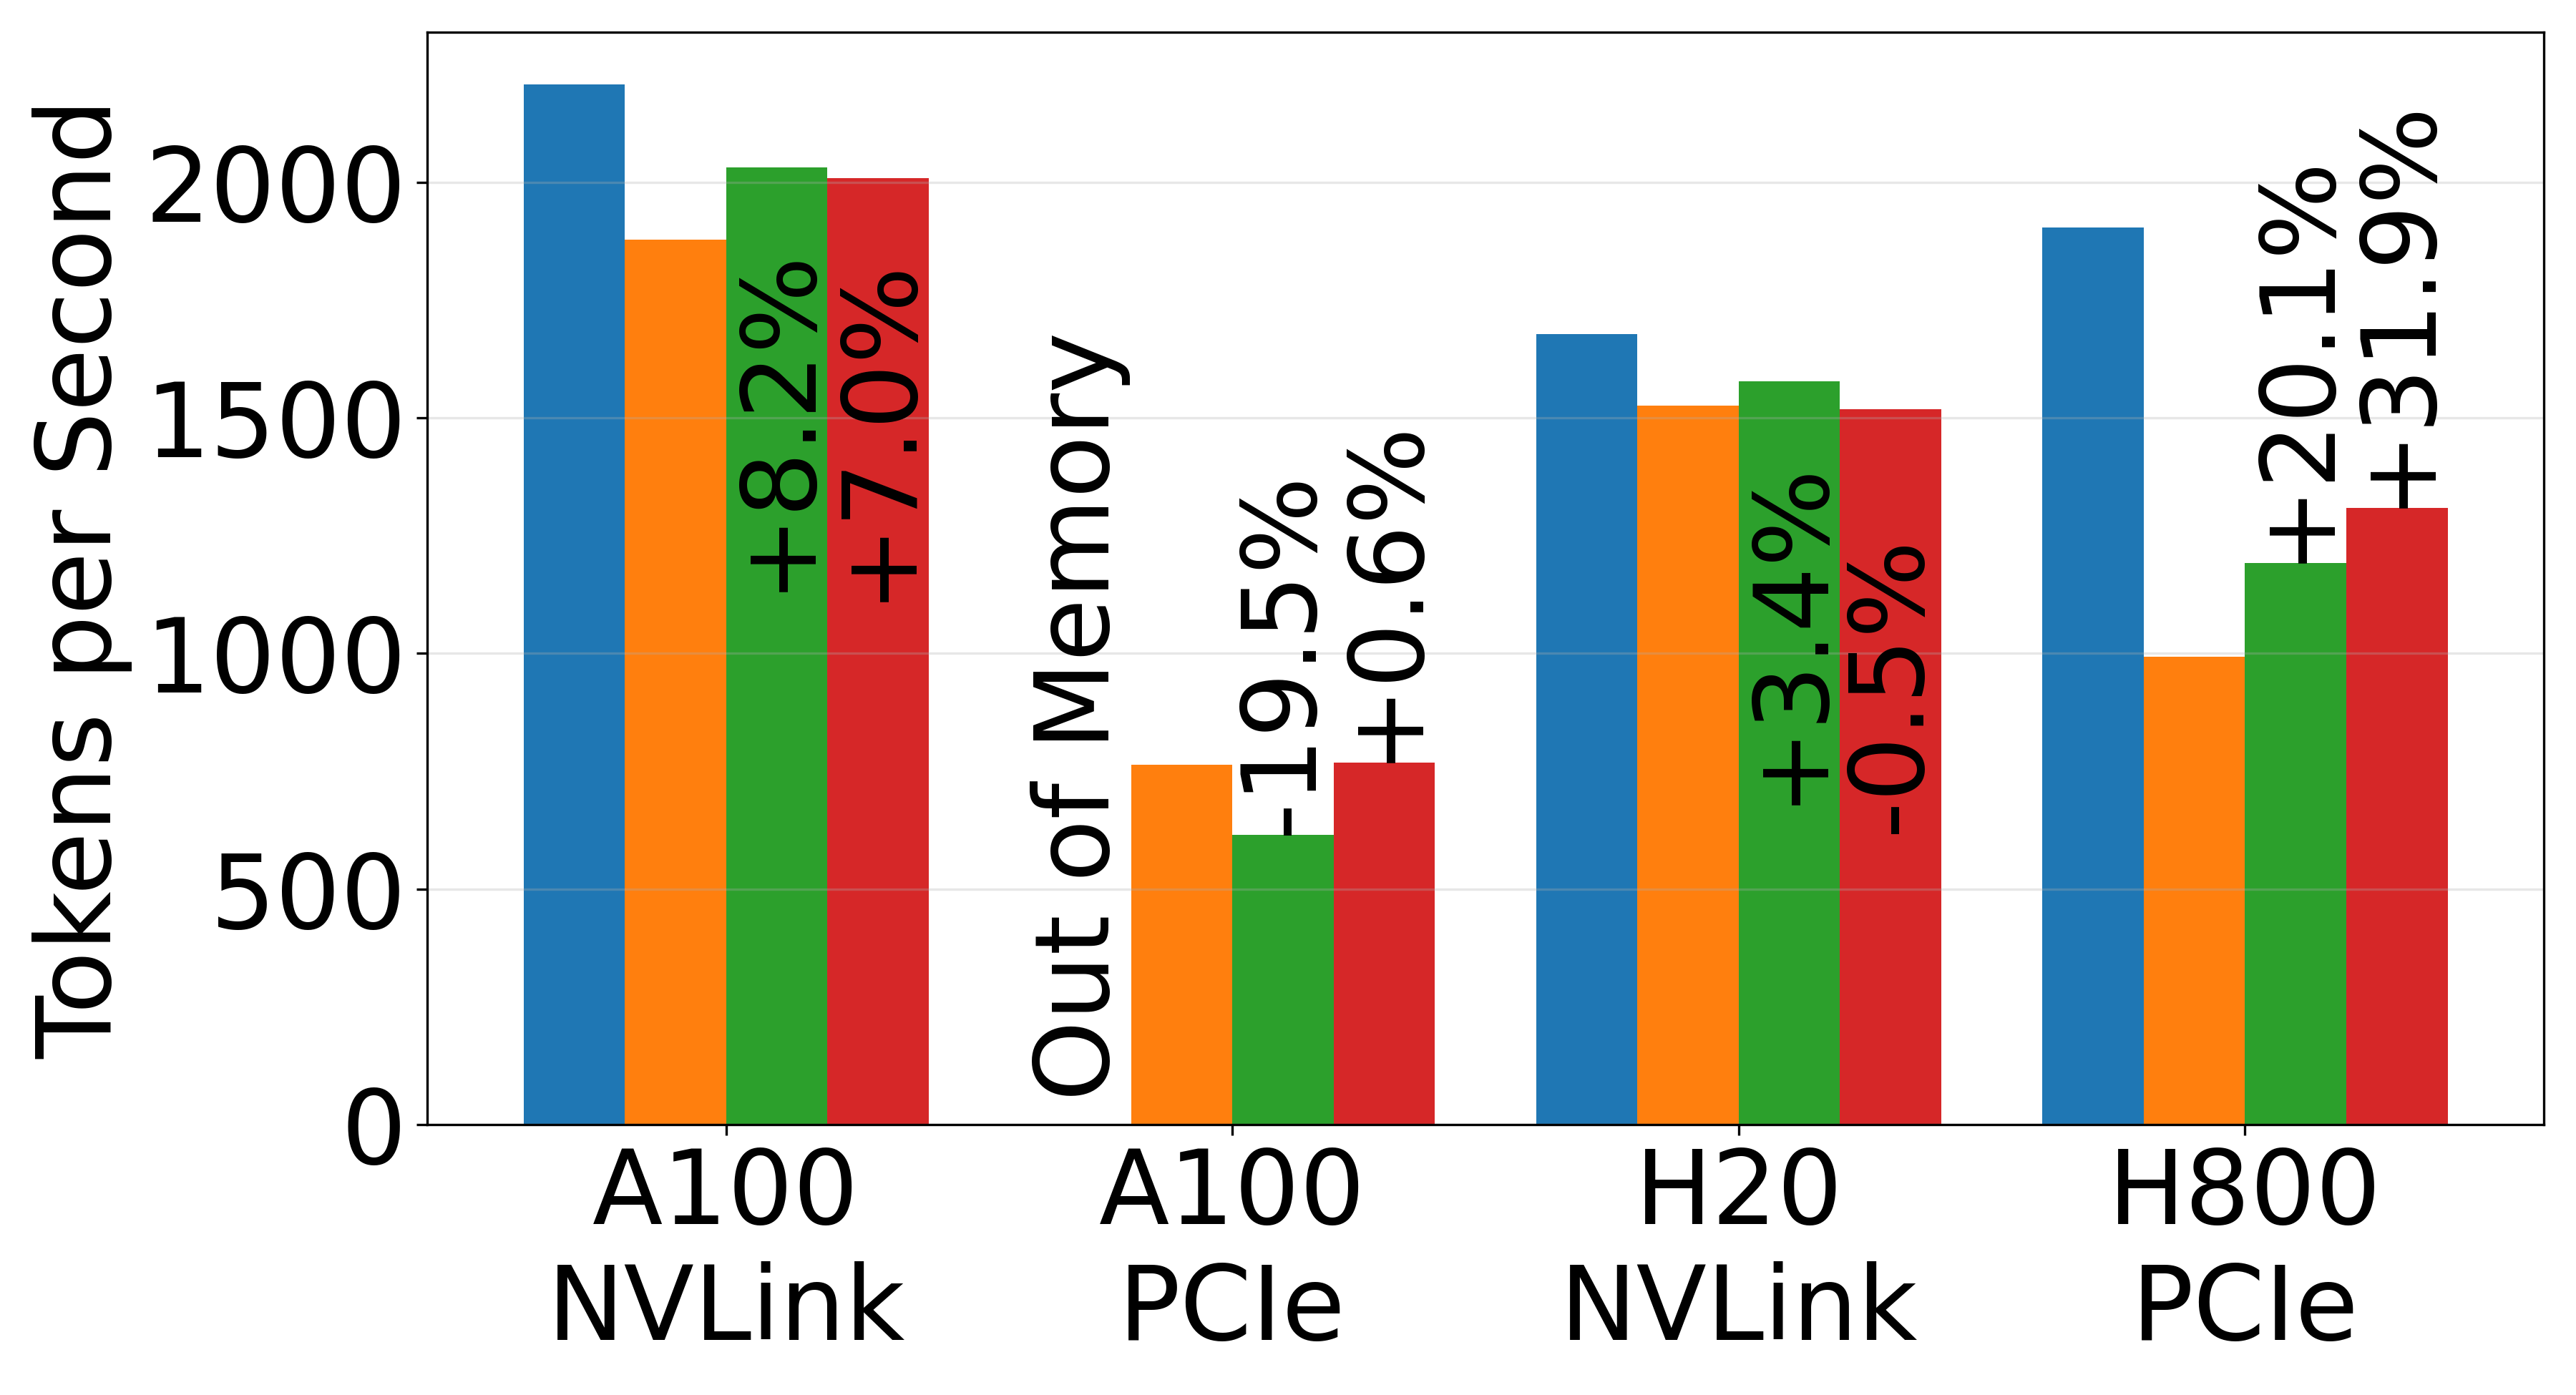
\includegraphics[width=\linewidth]{figures/hardware_comparison_b1_s2048_tokens_per_sec_qwen3-8b.png}
    \vspace{-1.5em}
    \caption{8B|B=128|S=2K}
  \end{subfigure}
  \begin{subfigure}{0.322\linewidth}
    \centering
    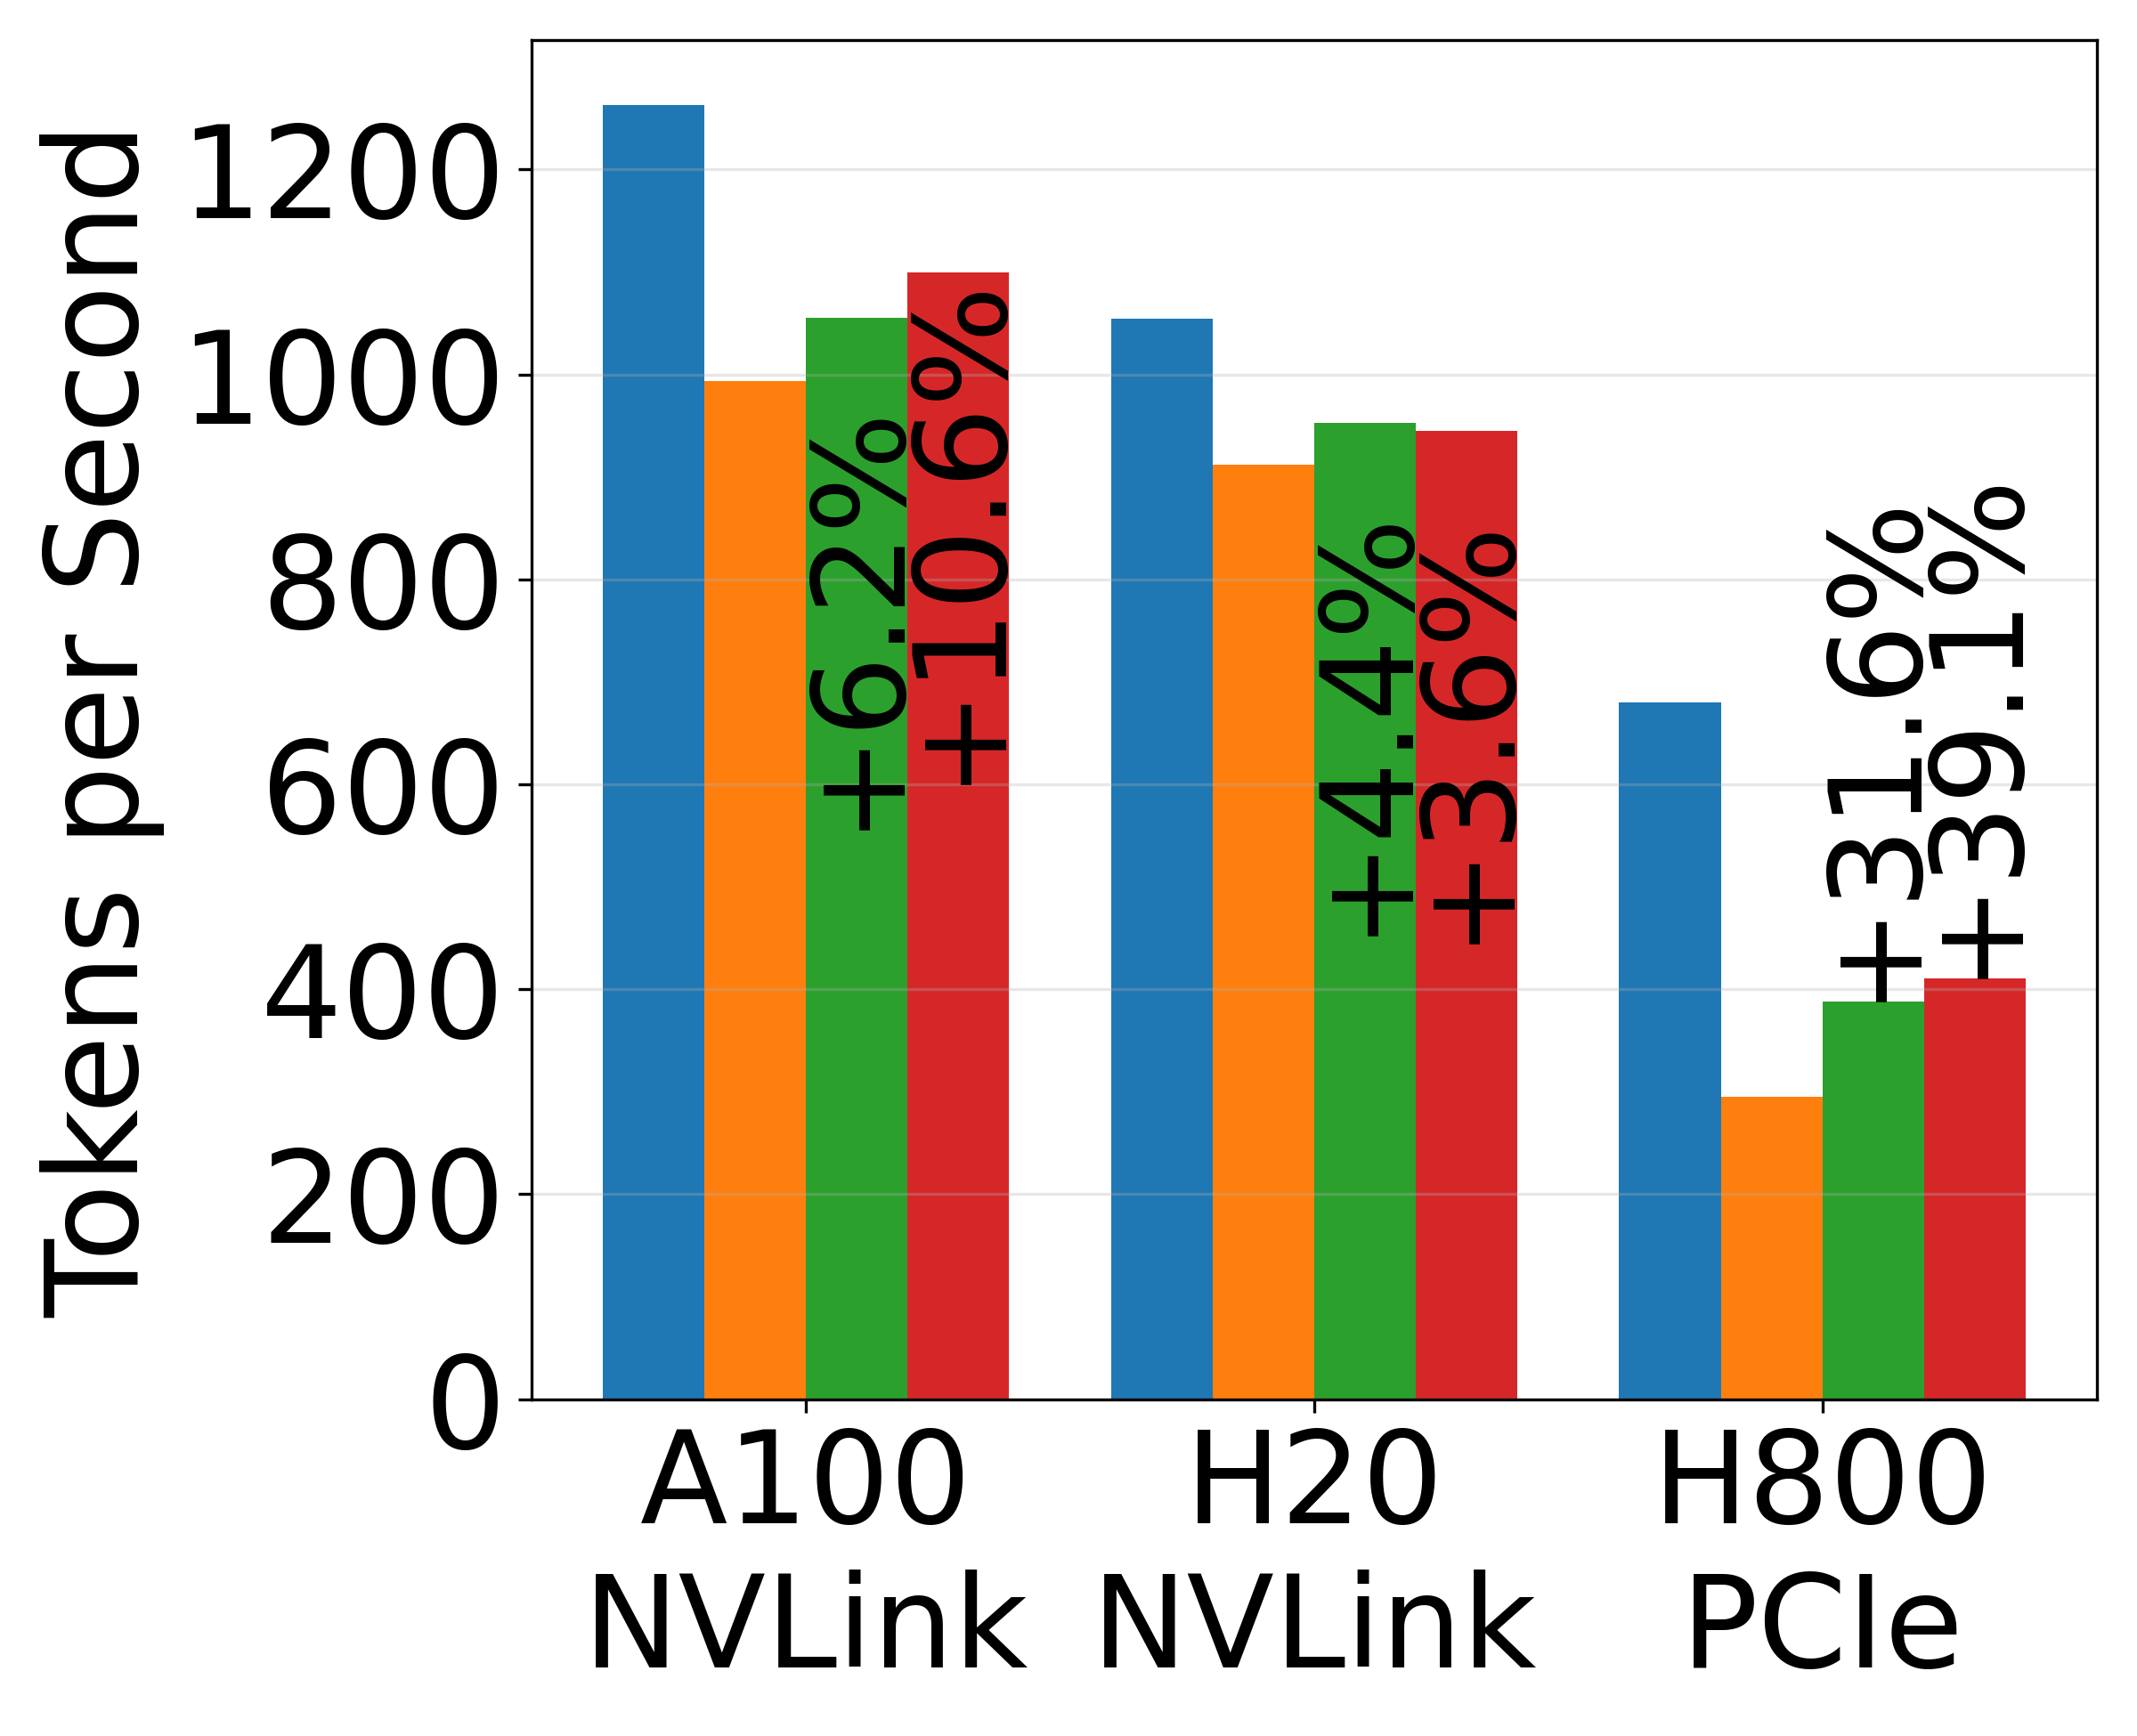
\includegraphics[width=\linewidth]{figures/hardware_comparison_b1_s1024_tokens_per_sec_qwen3-14b.png}
    \vspace{-1.5em}
    \caption{14B|B=128|S=1K}
  \end{subfigure}
  \begin{subfigure}{0.322\linewidth}
    \centering
    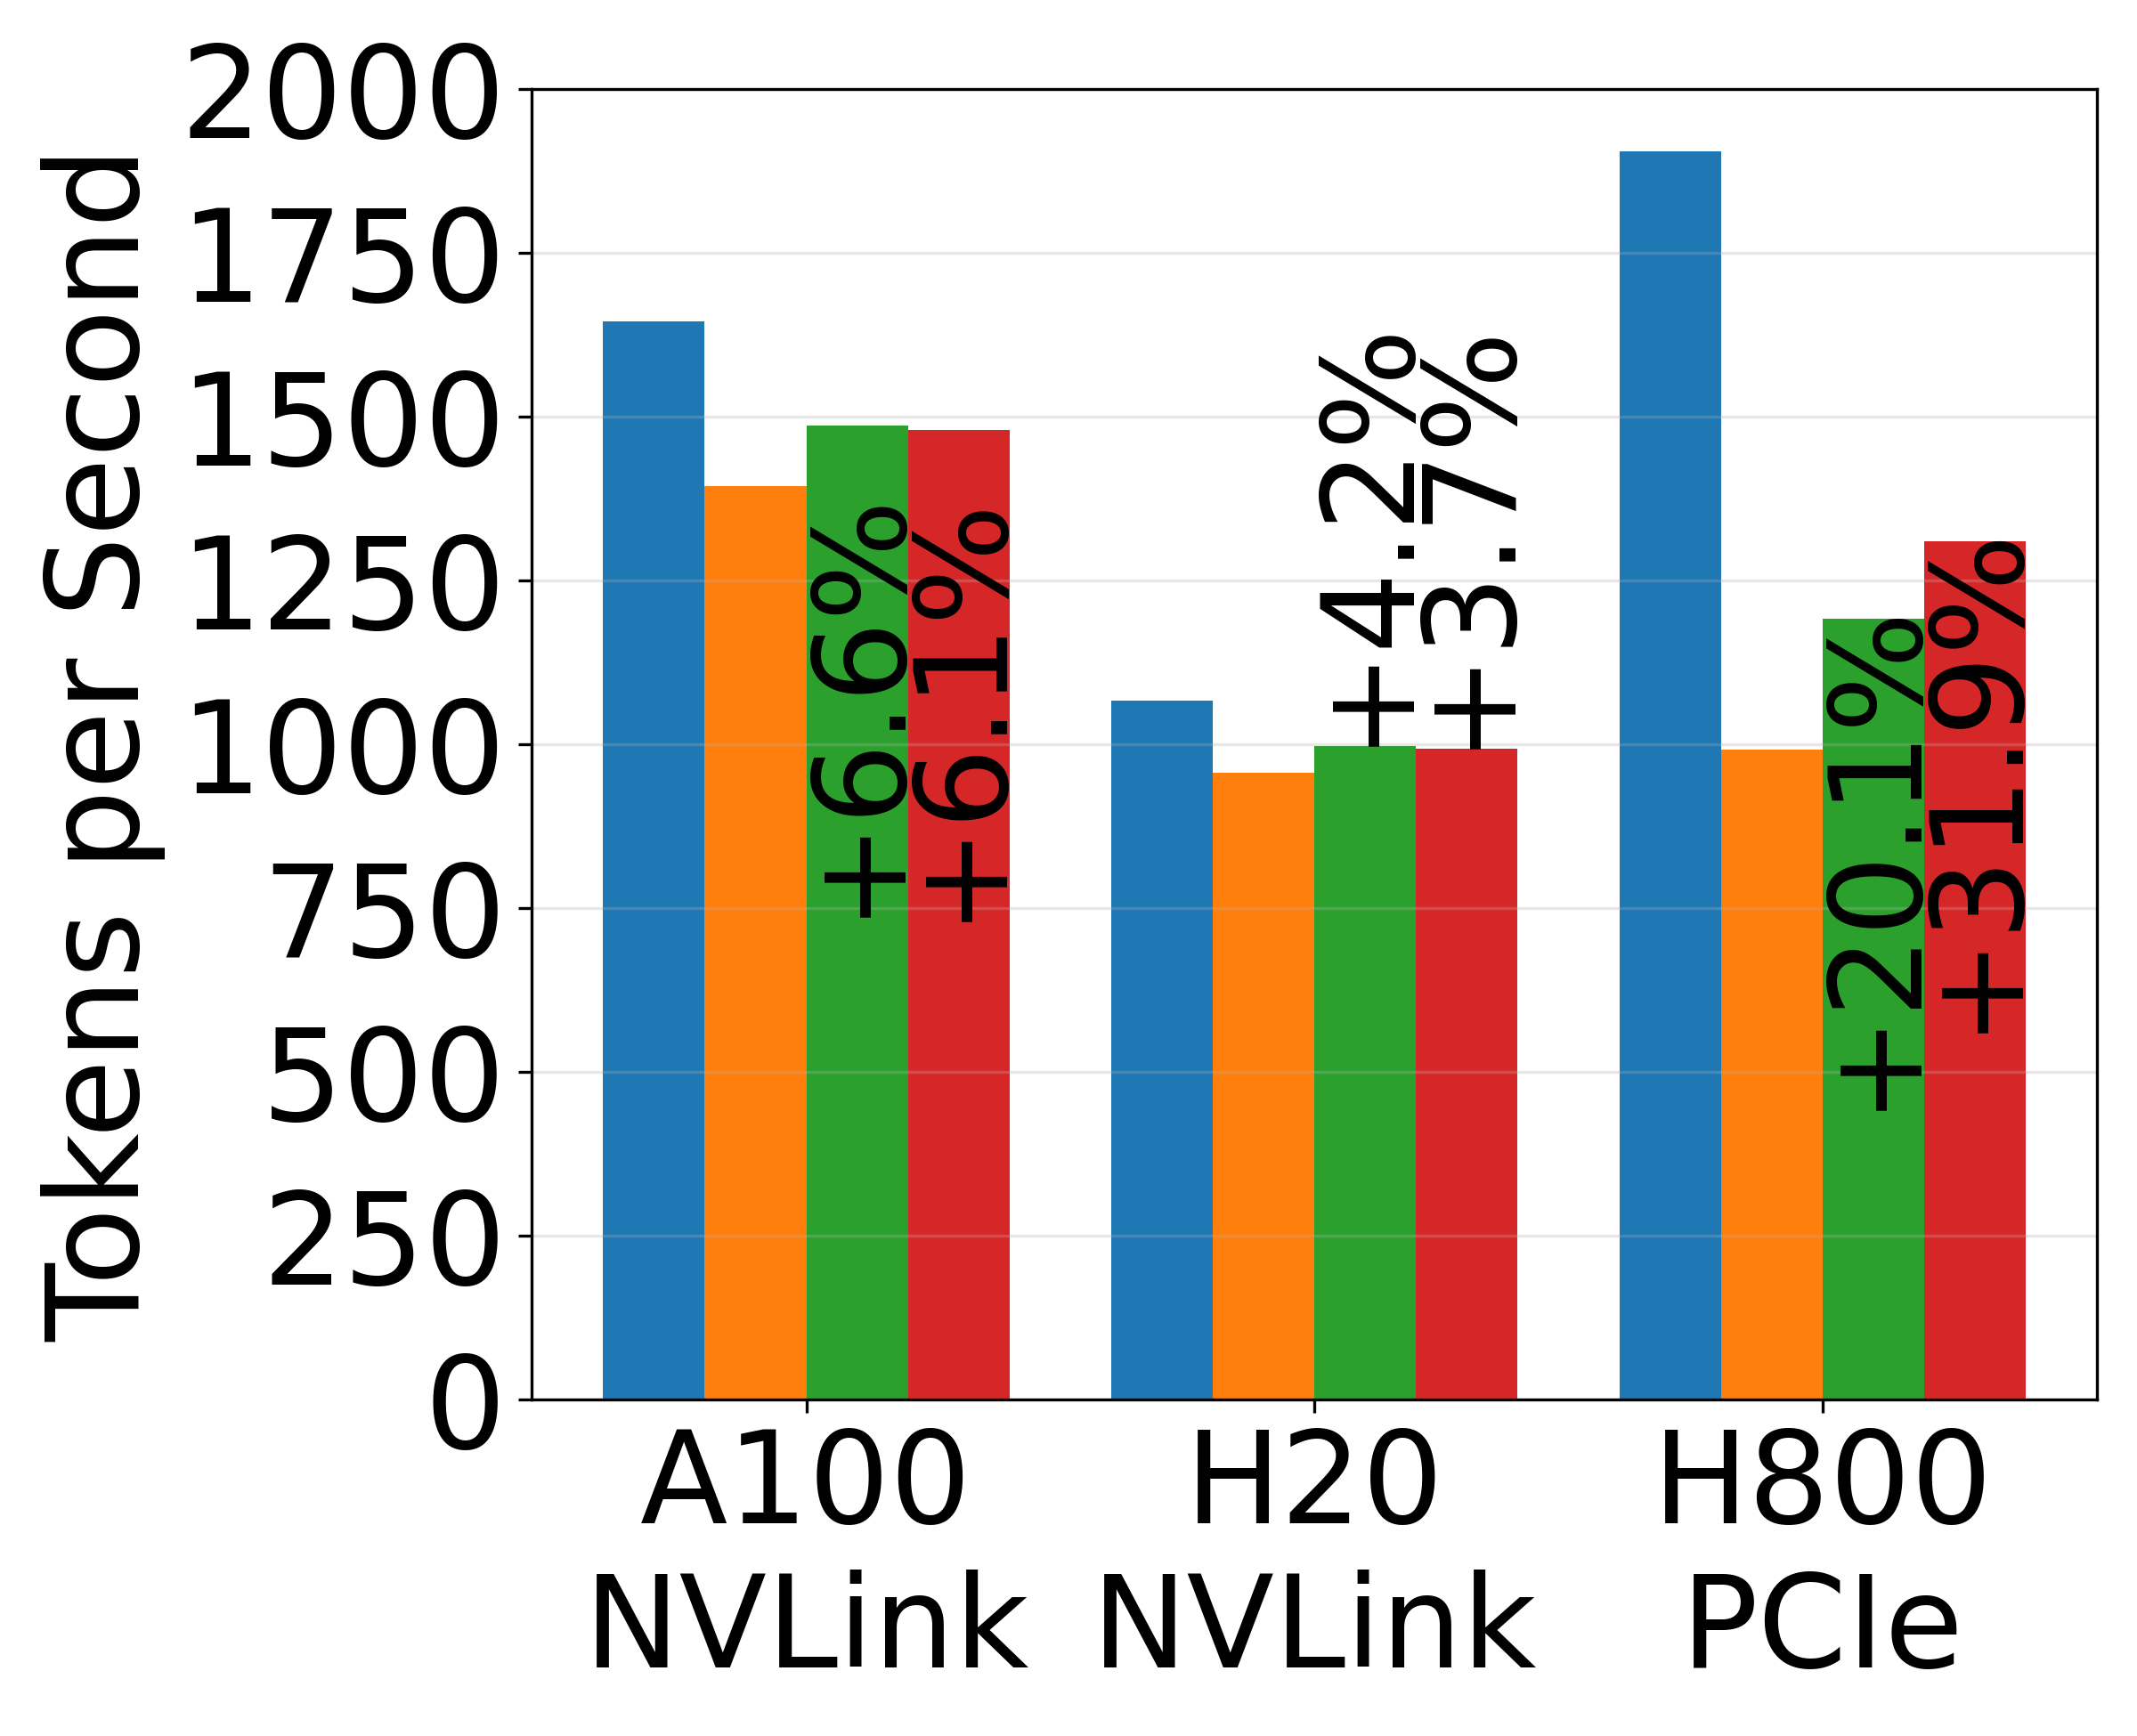
\includegraphics[width=\linewidth]{figures/hardware_comparison_b1_s2048_tokens_per_sec_qwen3-14b.png}
    \vspace{-1.5em}
    \caption{14B|B=128|S=2K}
  \end{subfigure}
  \begin{subfigure}{0.336\linewidth}
    \centering
    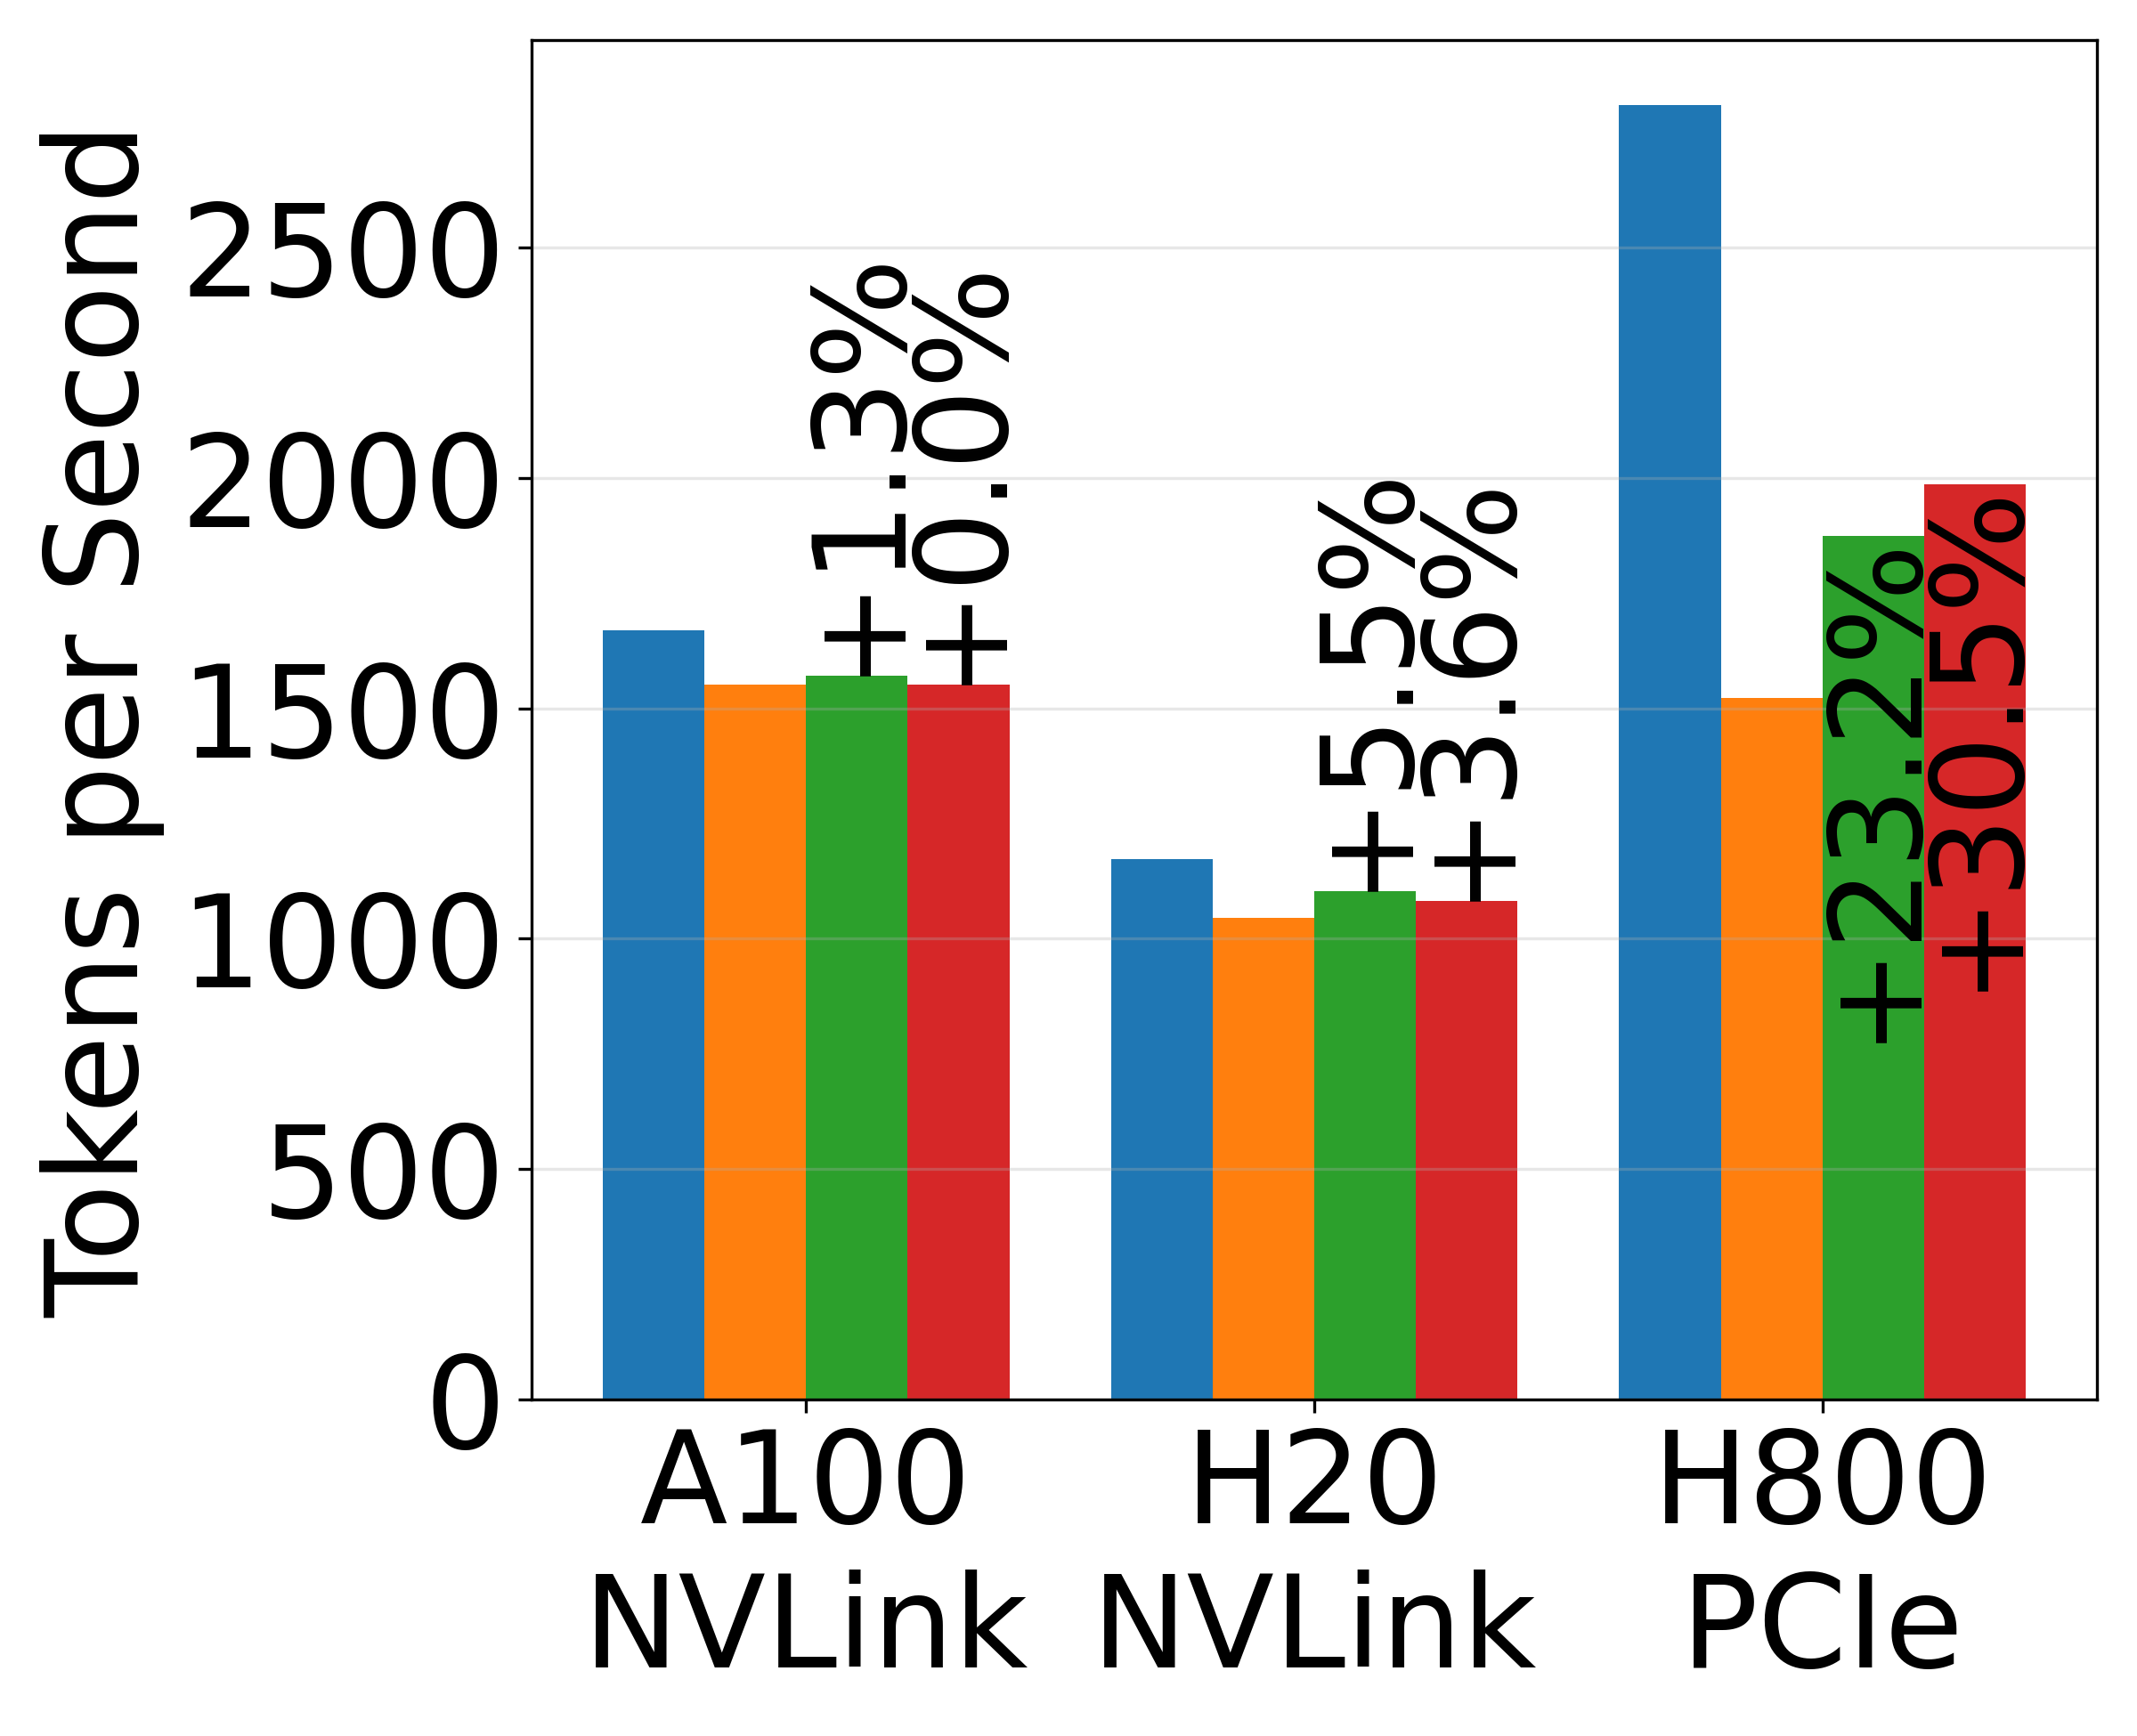
\includegraphics[width=0.972\linewidth]{figures/hardware_comparison_b2_s1536_tokens_per_sec_qwen3-14b.png}
    \vspace{-1.5em}
    \caption{14B|B=256|S=1.5K}
  \end{subfigure}
  \begin{subfigure}{0.515\linewidth}
    \centering
    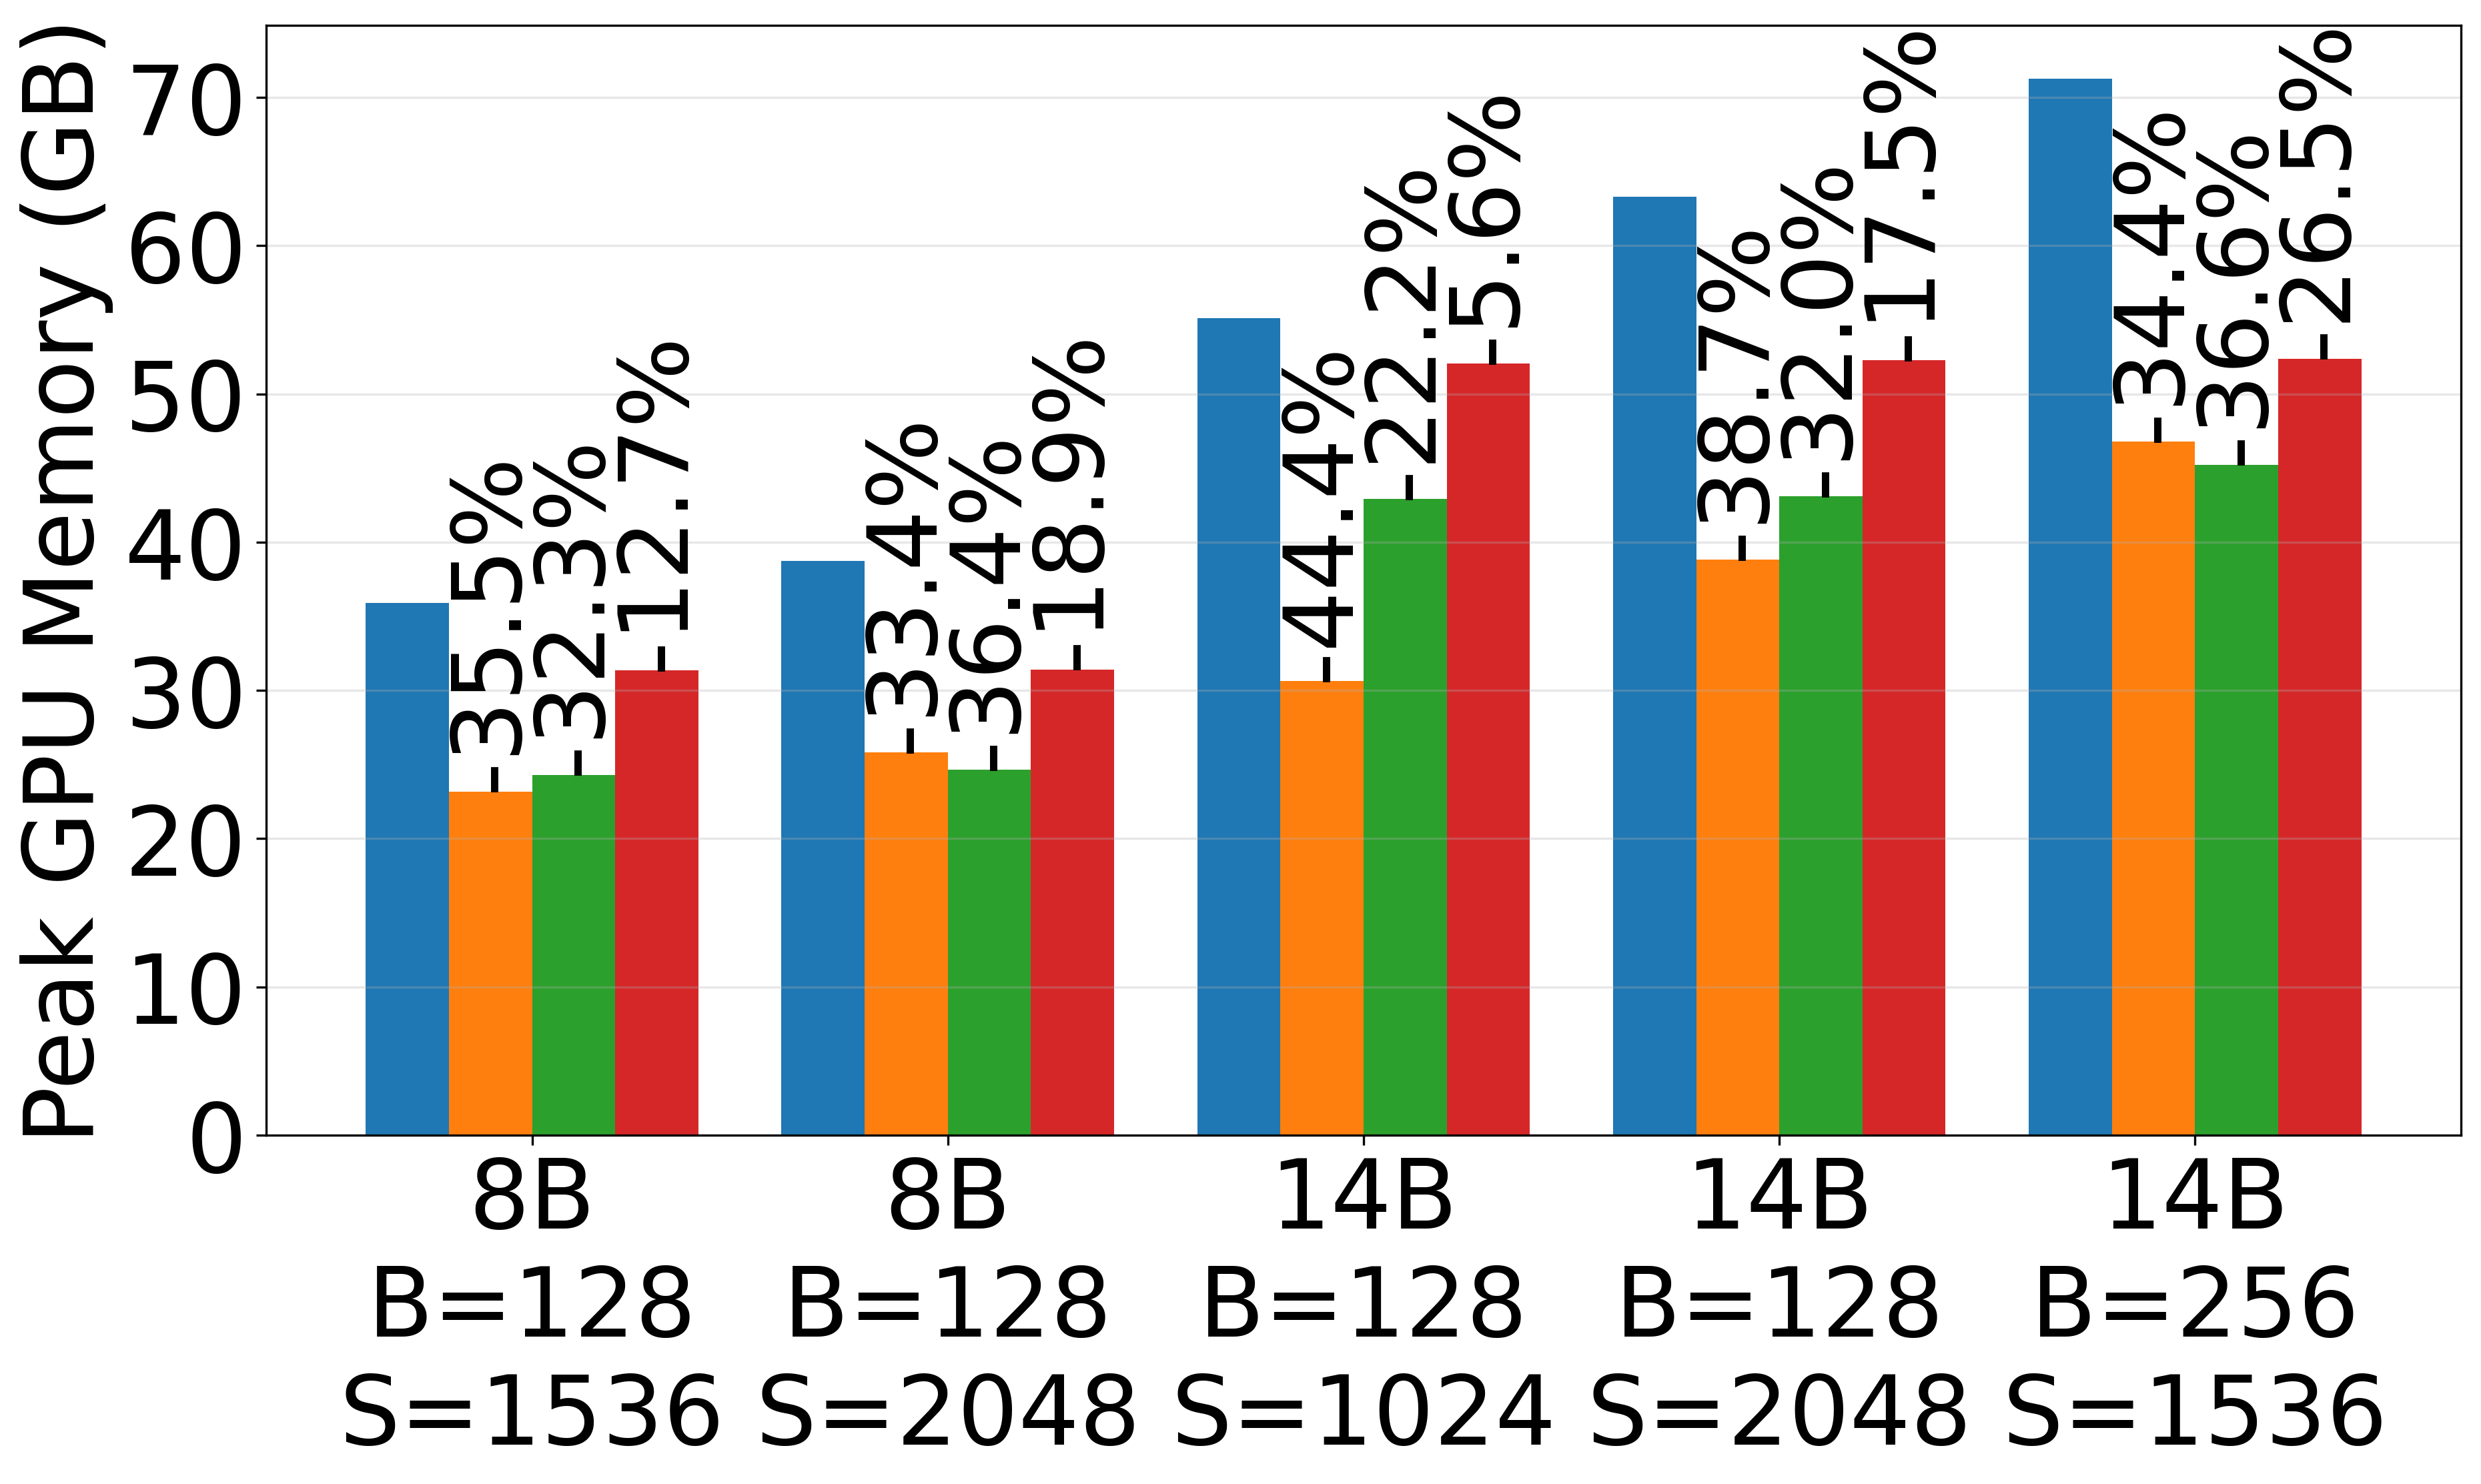
\includegraphics[width=\linewidth]{figures/memory_comparison_a100_nvlink.png}
    \vspace{-1.5em}
    \caption{Peak Memory (vs ZeRO-2)}
  \end{subfigure}
  \begin{subfigure}{0.475\linewidth}
    \centering
    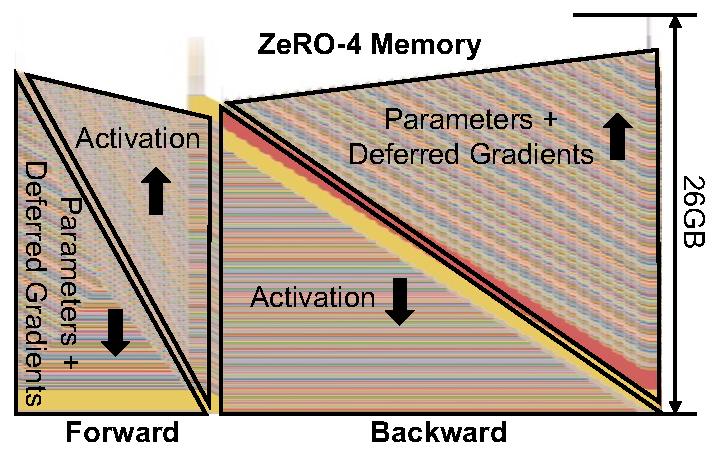
\includegraphics[width=\linewidth]{figures/zero4_memory.pdf}
    \vspace{-1.5em}
    \caption{Memory Snapshot}
  \end{subfigure}
  \vspace{-1.7em}
  \caption{Comparison of ZeRO-2, ZeRO-3, ZeRO-3.5, and ZeRO-4 in terms of performance (baseline: ZeRO-3) and memory footprint (baseline: ZeRO-2).}
  \vspace{-2em}
  \label{fig:zero_comparison}
\end{figure}

\subsection{Evaluation on New ZeRO Strategies}
\label{sec:exp_zeros}

\subsubsection{Performance and Memory Comparison}
\label{sec:zero_performance}

Fig.~\ref{fig:zero_comparison} compares the performance and memory footprint of ZeRO-2, ZeRO-3, ZeRO-3.5, and ZeRO-4 across different hardware and model settings. These experiments use 8 GPUs, 16 accumulation steps, and micro-batch sizes per device of 1 and 2 (total batch sizes 128 and 256). Results for Qwen3-14B on A100-PCIe (40\,GB) are omitted due to OOM in most configurations. In ZeRO-3.5 (Fig.~\ref{fig:FSDP}(c)), the backward pass reuses activation memory that is progressively released to hold gathered weight shards; the gathered weights are discarded in the subsequent forward step to free space for activations. This preserves ZeRO-3's peak memory (Fig.~\ref{fig:zero_comparison}(f)) while eliminating forward all-gather communication, resulting in up to a 31.6\% throughput improvement over ZeRO-3 (Fig.~\ref{fig:zero_comparison}(c)). ZeRO-4 further retains a portion of unreduced gradient buckets in the freed activation memory and defers their reduce-scatter to the next forward pass (Fig.~\ref{fig:FSDP}(d)). By shifting part of the backward communication into the forward pass and overlapping it with forward computation, ZeRO-4 achieves more balanced communication and up to a 39.1\% throughput improvement.

Fig.~\ref{fig:zero_comparison}(g) shows a memory snapshot of ZeRO-4 for Qwen3-8B (batch size = 256; seq\_len = 1.5K; memory for optimizer states, 32-bit parameters, and gradients is omitted since these are identical across strategies): peak activation memory = 26\,GB; total 16-bit parameter memory = 16\,GB; and 1/4 of gradient buckets deferred to the next forward pass, so parameters plus deferred gradients occupy 21\,GB. Let $P$ denote parameter memory, $\alpha$ the fraction of parameters retained during the backward pass, and $\beta$ the fraction of gradients deferred to the next forward pass. If the activation peak $A$ satisfies $A \ge (\alpha+\beta)\cdot P$, then the peak memory usage of ZeRO-3, ZeRO-3.5, and ZeRO-4 is comparable (Fig.~\ref{fig:zero_comparison}(f)). 

% Hence, without increasing peak GPU memory (up to 36.5\% savings compared to ZeRO-2), these strategies can improve memory utilization and trade memory for up to a 40\% increase in throughput.

From a hardware perspective, as shown in Fig.~\ref{fig:zero_comparison}(a-d), the performance gains of ZeRO-3.5 and ZeRO-4 over ZeRO-3 are more pronounced on systems with lower communication bandwidth (e.g., PCIe vs. NVLink) and under lighter compute loads (since communication overhead is harder to overlap). ZeRO-3.5 eliminates the forward all-gather, and ZeRO-4 further shifts part of backward communication into the forward pass (with no forward communication in ZeRO-3.5) to improve communication-computation overlap, thereby yielding larger performance improvements on communication-constrained systems.

\subsubsection{Configuration Exploration}

We further analyze how hyperparameters affect the performance and memory usage of ZeRO-3.5 and ZeRO-4. We vary batch size/sequence length (to vary activation memory and computation loads) and strategy-specific hyperparameters: the ratio between retained gathered parameters and released parameters during backward (ZeRO-3.5), and the ratio between reduced gradient buckets and buckets whose gradient reduce-scatter is deferred to the subsequent forward pass (ZeRO-4). For ZeRO-4 exploration, we fix the retained-parameter ratio to \texttt{ALL:0} (all gathered parameters are kept during backward).

\begin{figure}[h]
  \centering
  \begin{subfigure}{0.48\linewidth}
    \centering
    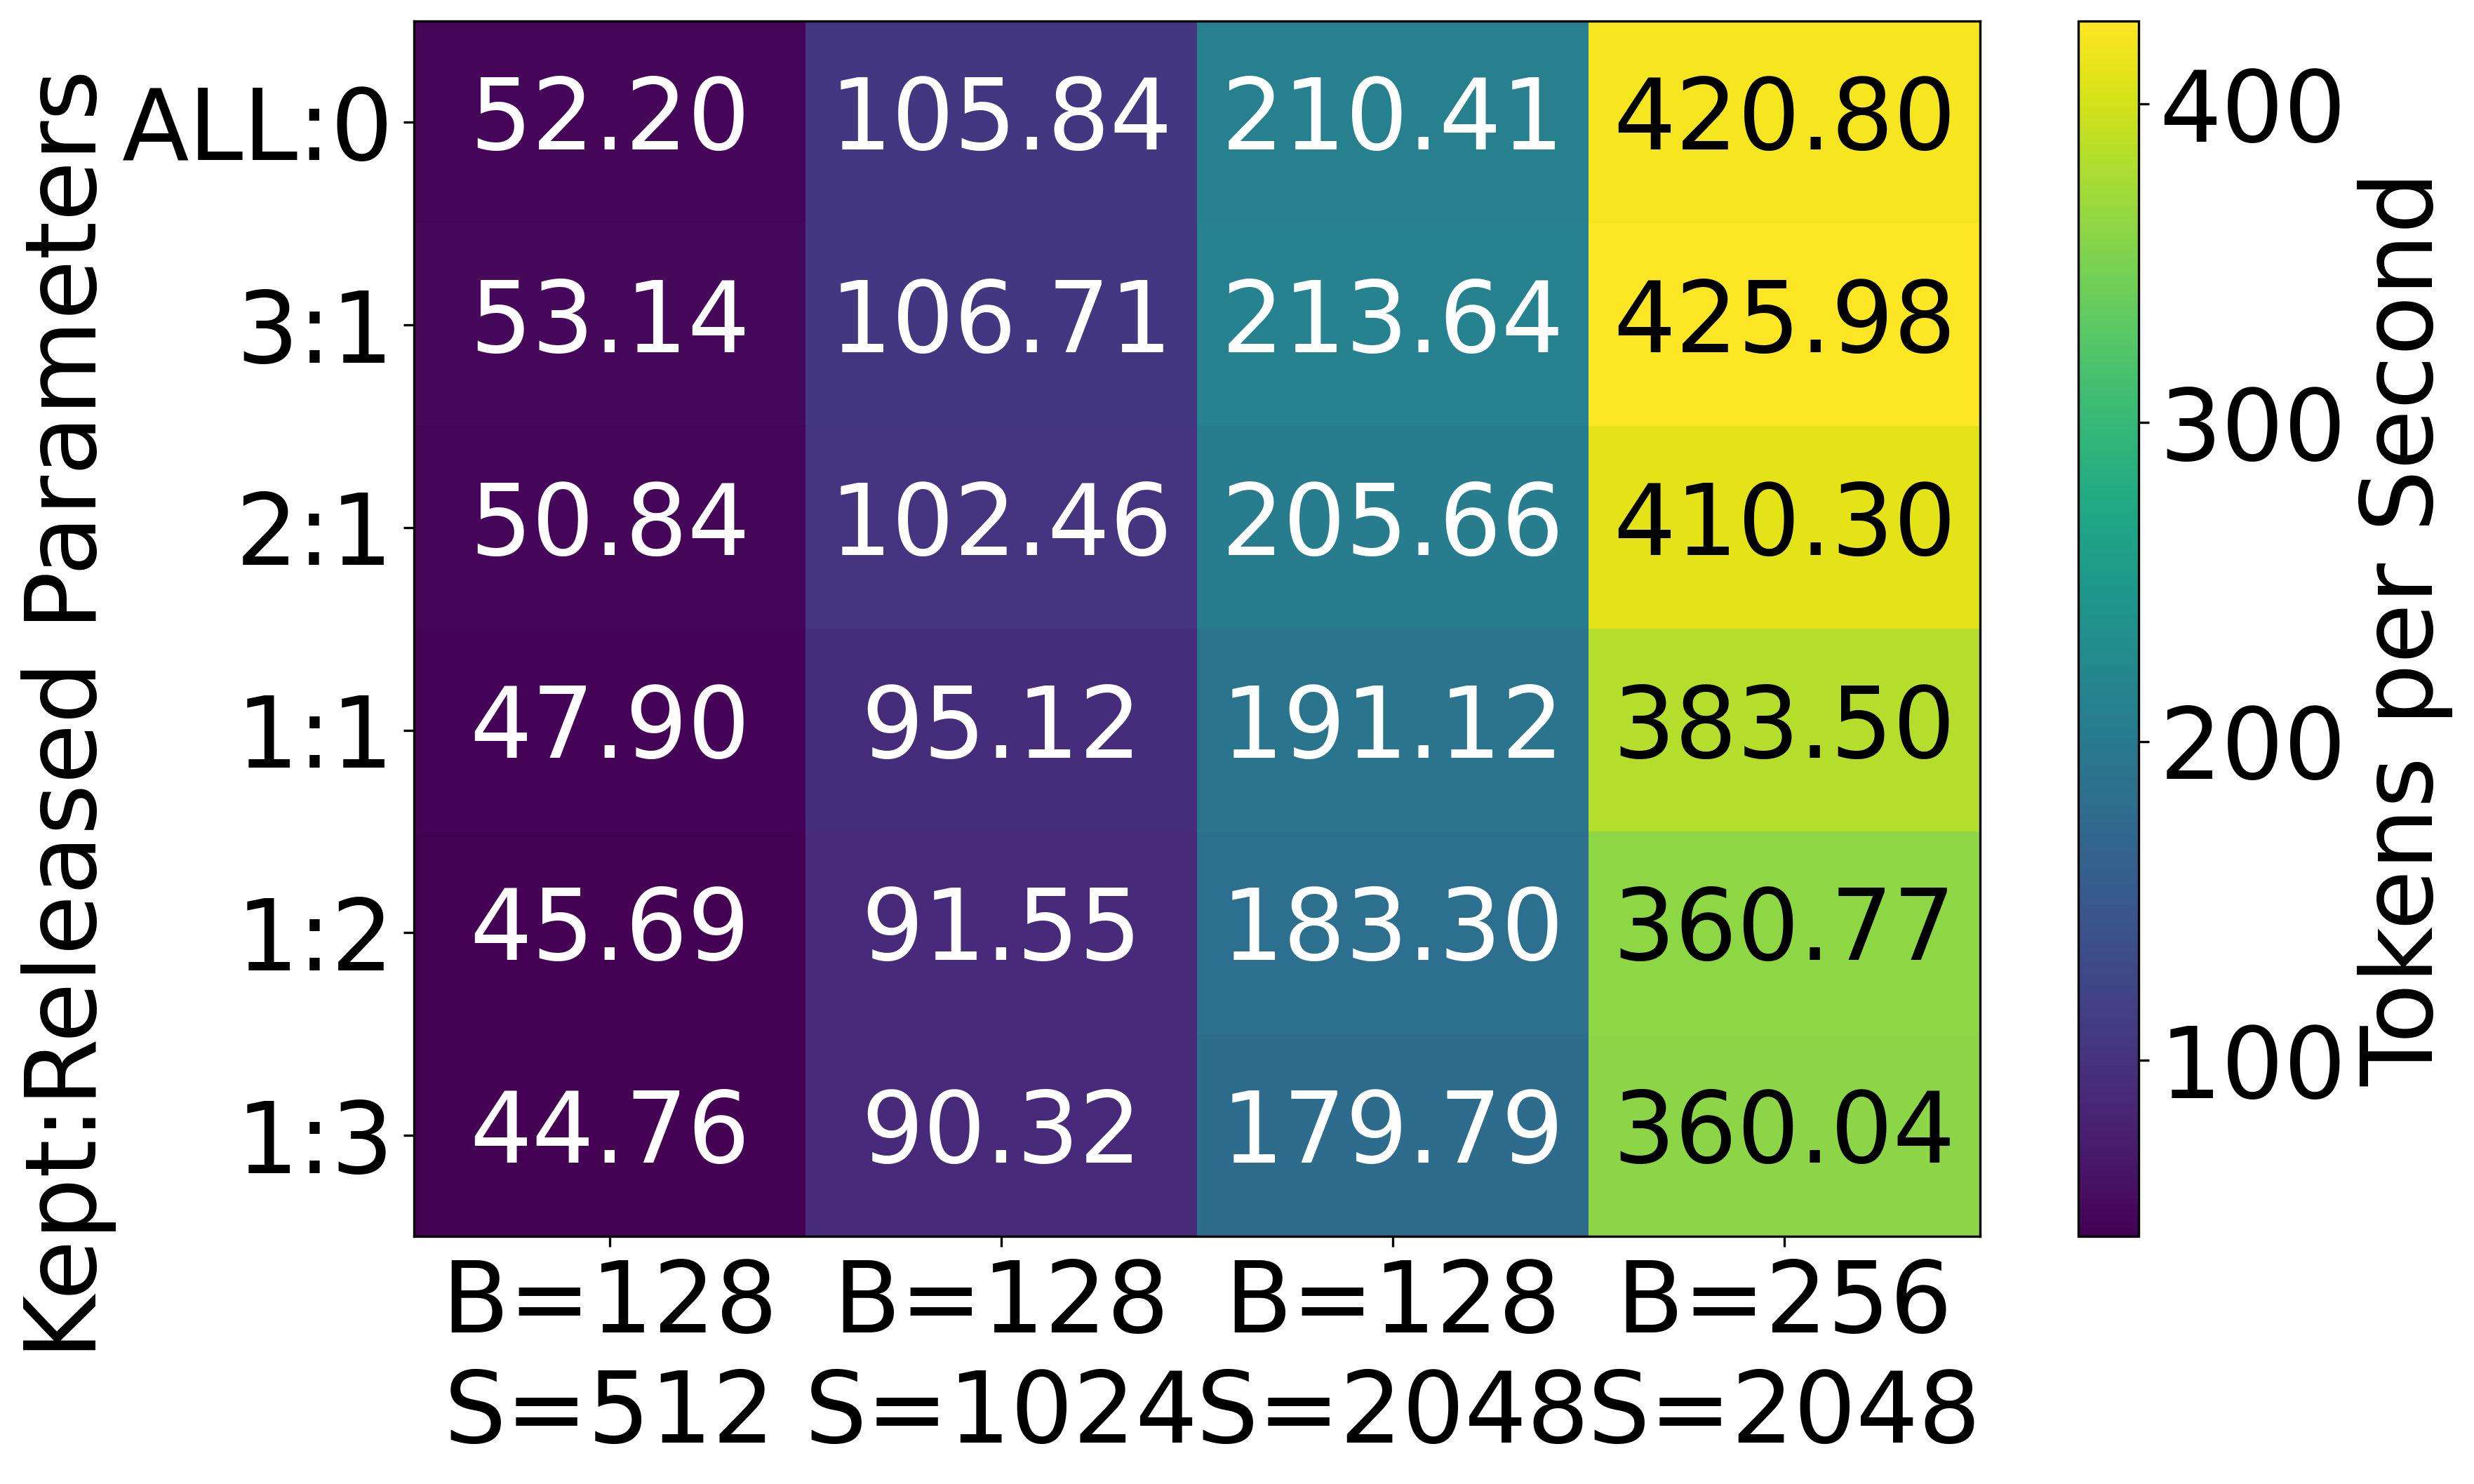
\includegraphics[width=\linewidth]{figures/strategy_3.5_ckpt_False_tokens_per_sec_heatmap.png}
    \vspace{-1.5em}
    \caption{Throughput (ZeRO-3.5)}
  \end{subfigure}
  \begin{subfigure}{0.48\linewidth}
    \centering
    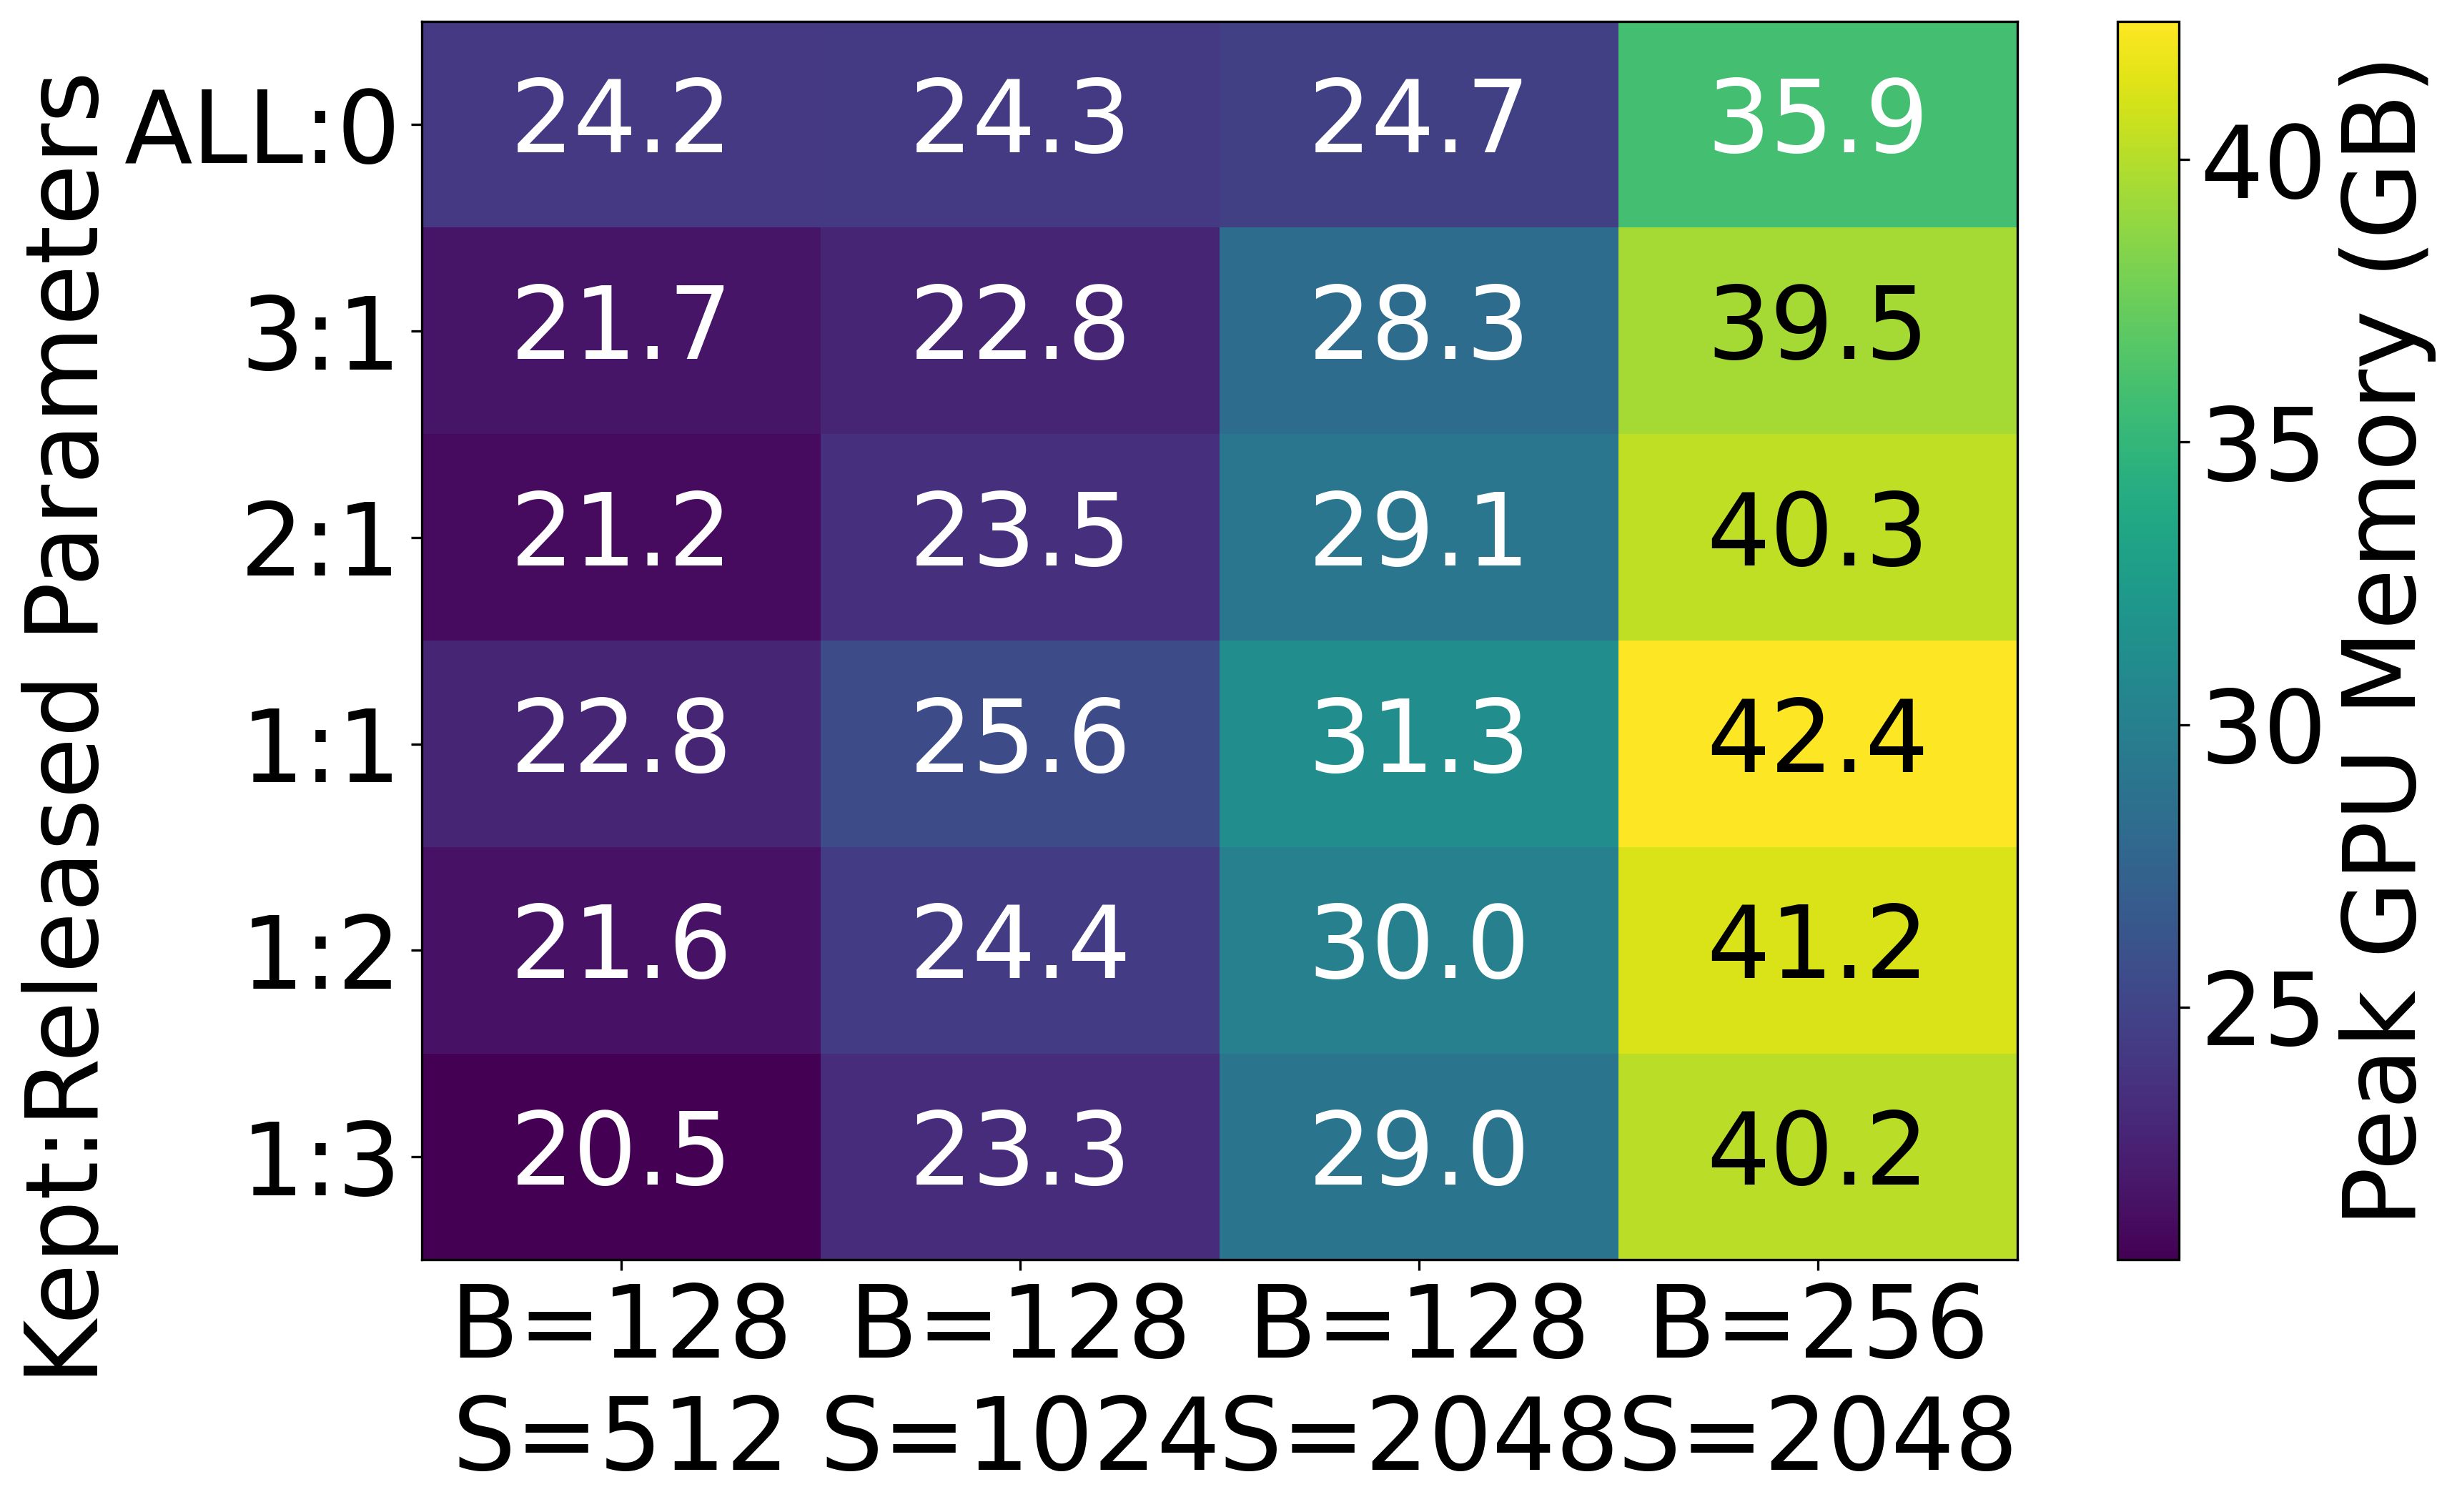
\includegraphics[width=\linewidth]{figures/strategy_3.5_ckpt_False_peak_gpu_mem_mb_heatmap.png}
    \vspace{-1.5em}
    \caption{Peak Memory (ZeRO-3.5)}
  \end{subfigure}
  \begin{subfigure}{0.48\linewidth}
    \centering
    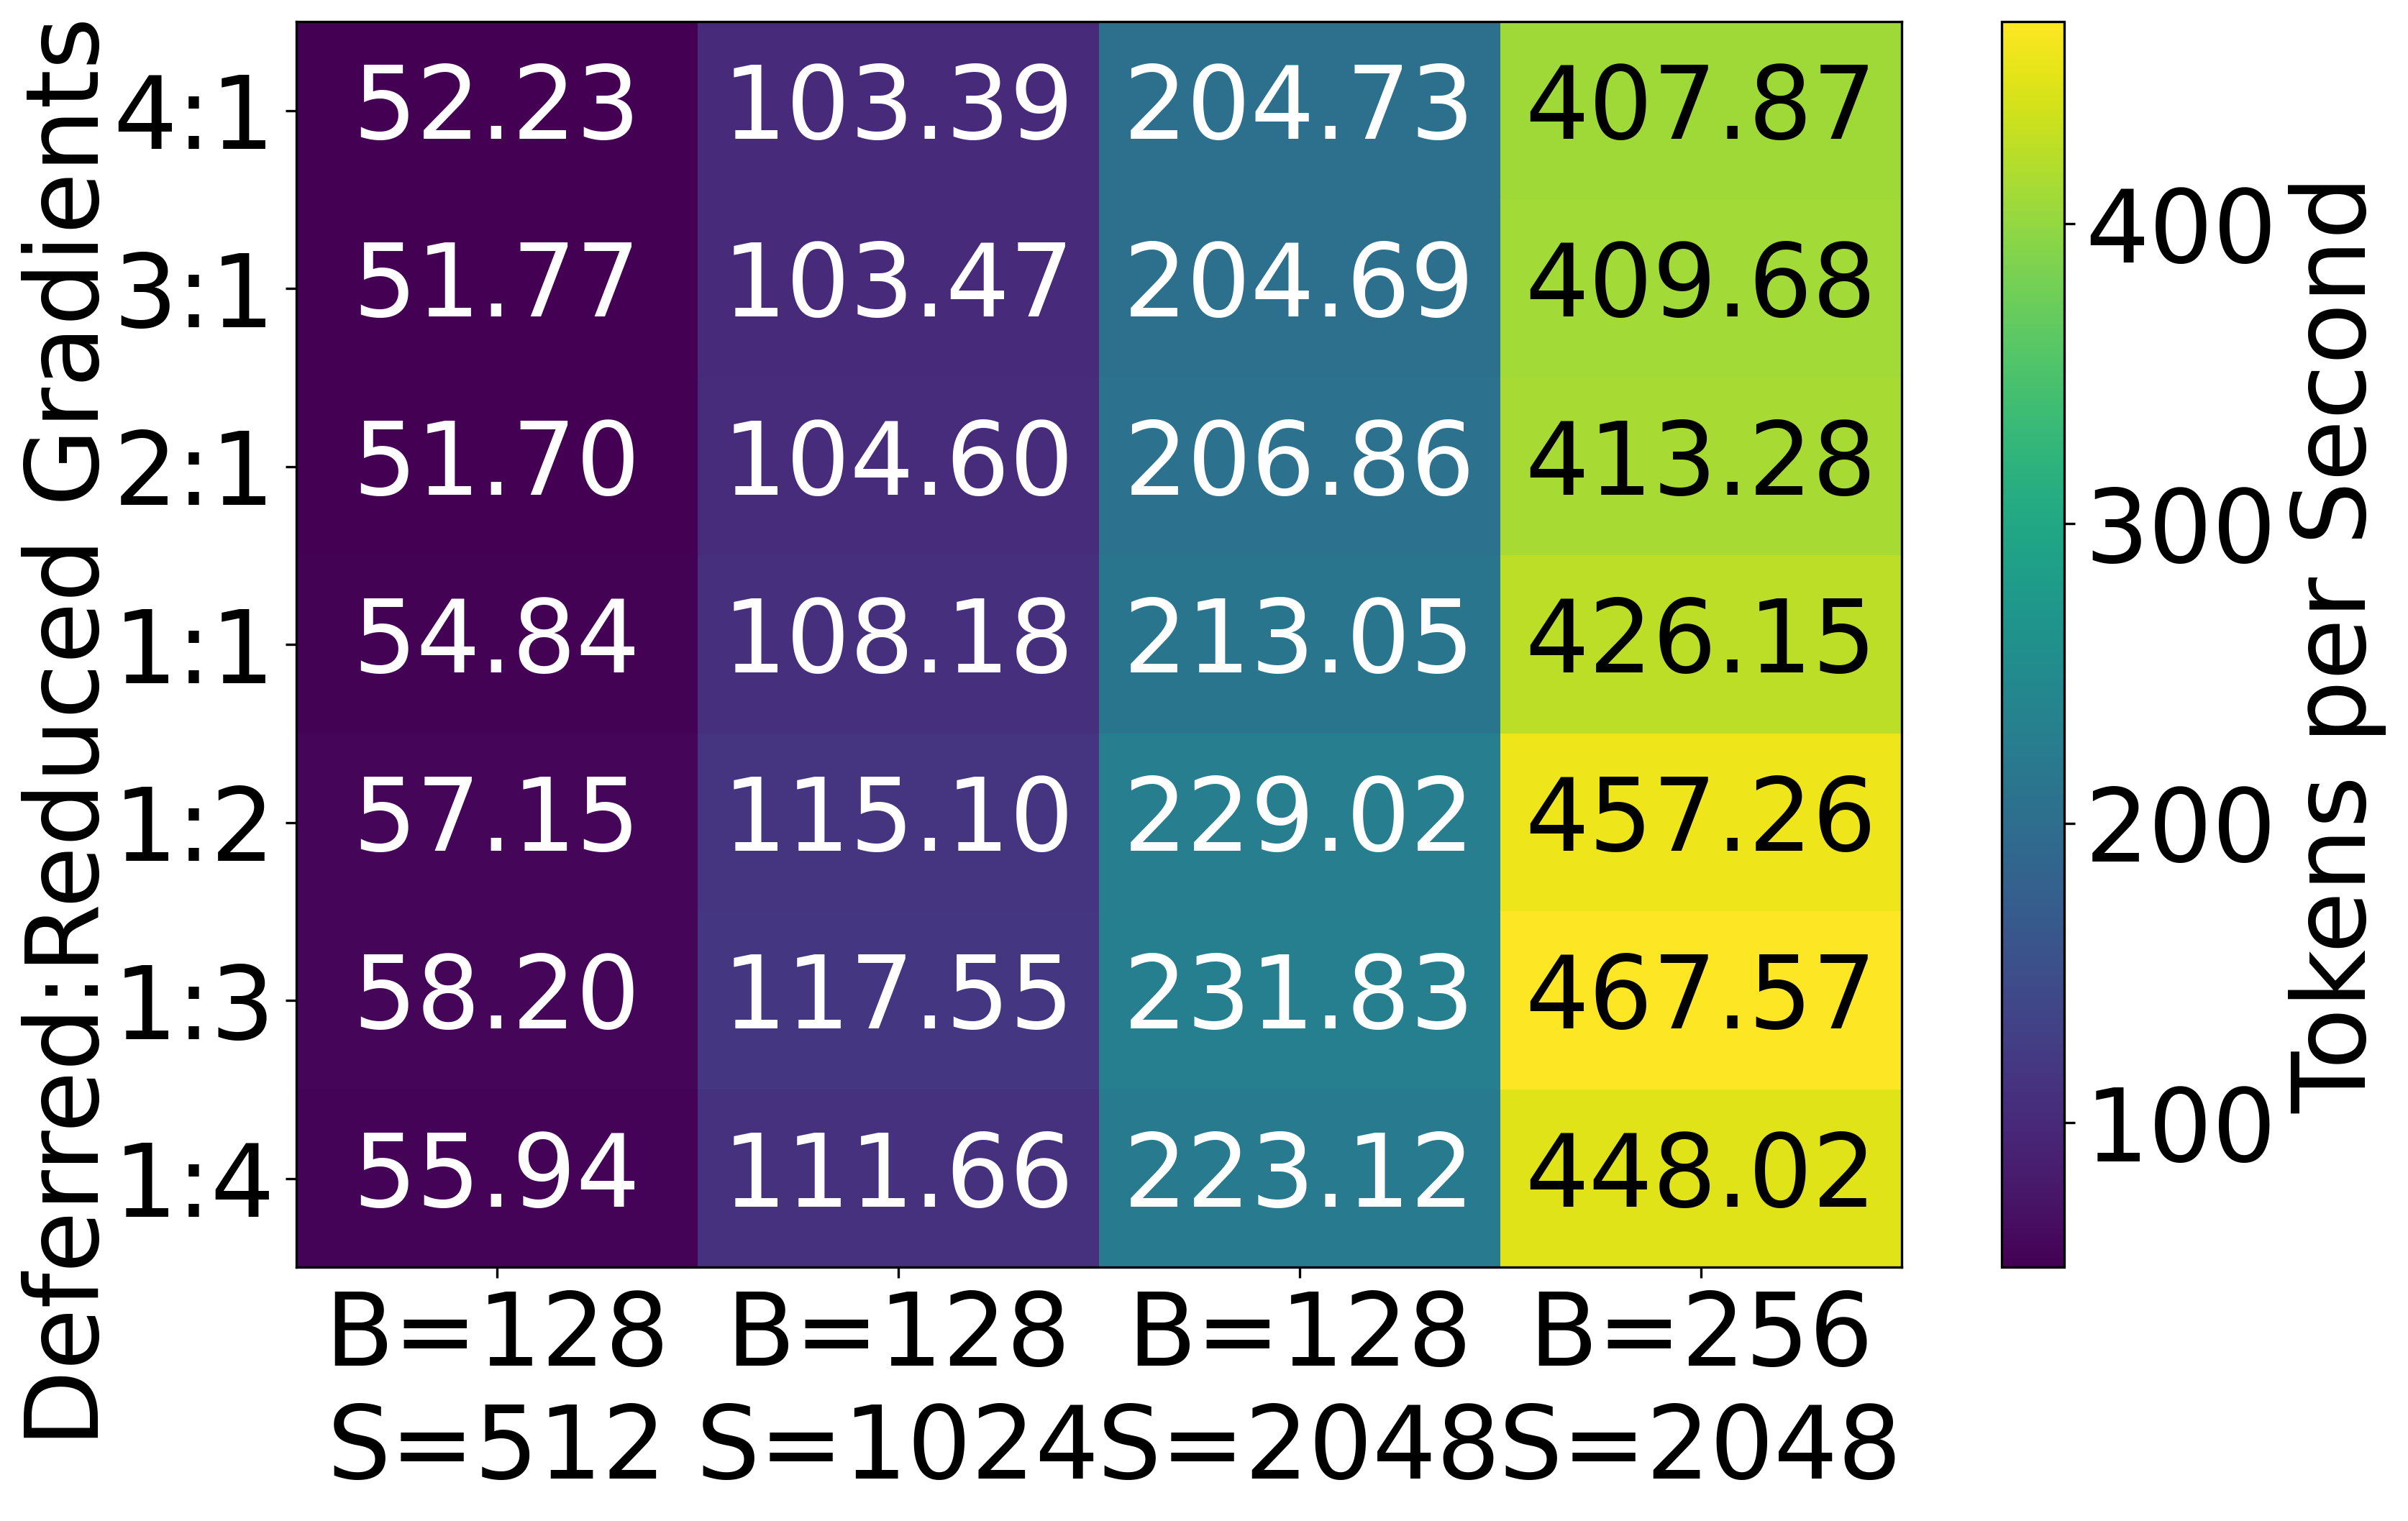
\includegraphics[width=\linewidth]{figures/strategy_4.0_ckpt_False_tokens_per_sec_heatmap.png}
    \vspace{-1.5em}
    \caption{Throughput (ZeRO-4)}
  \end{subfigure}
  \begin{subfigure}{0.48\linewidth}
    \centering
    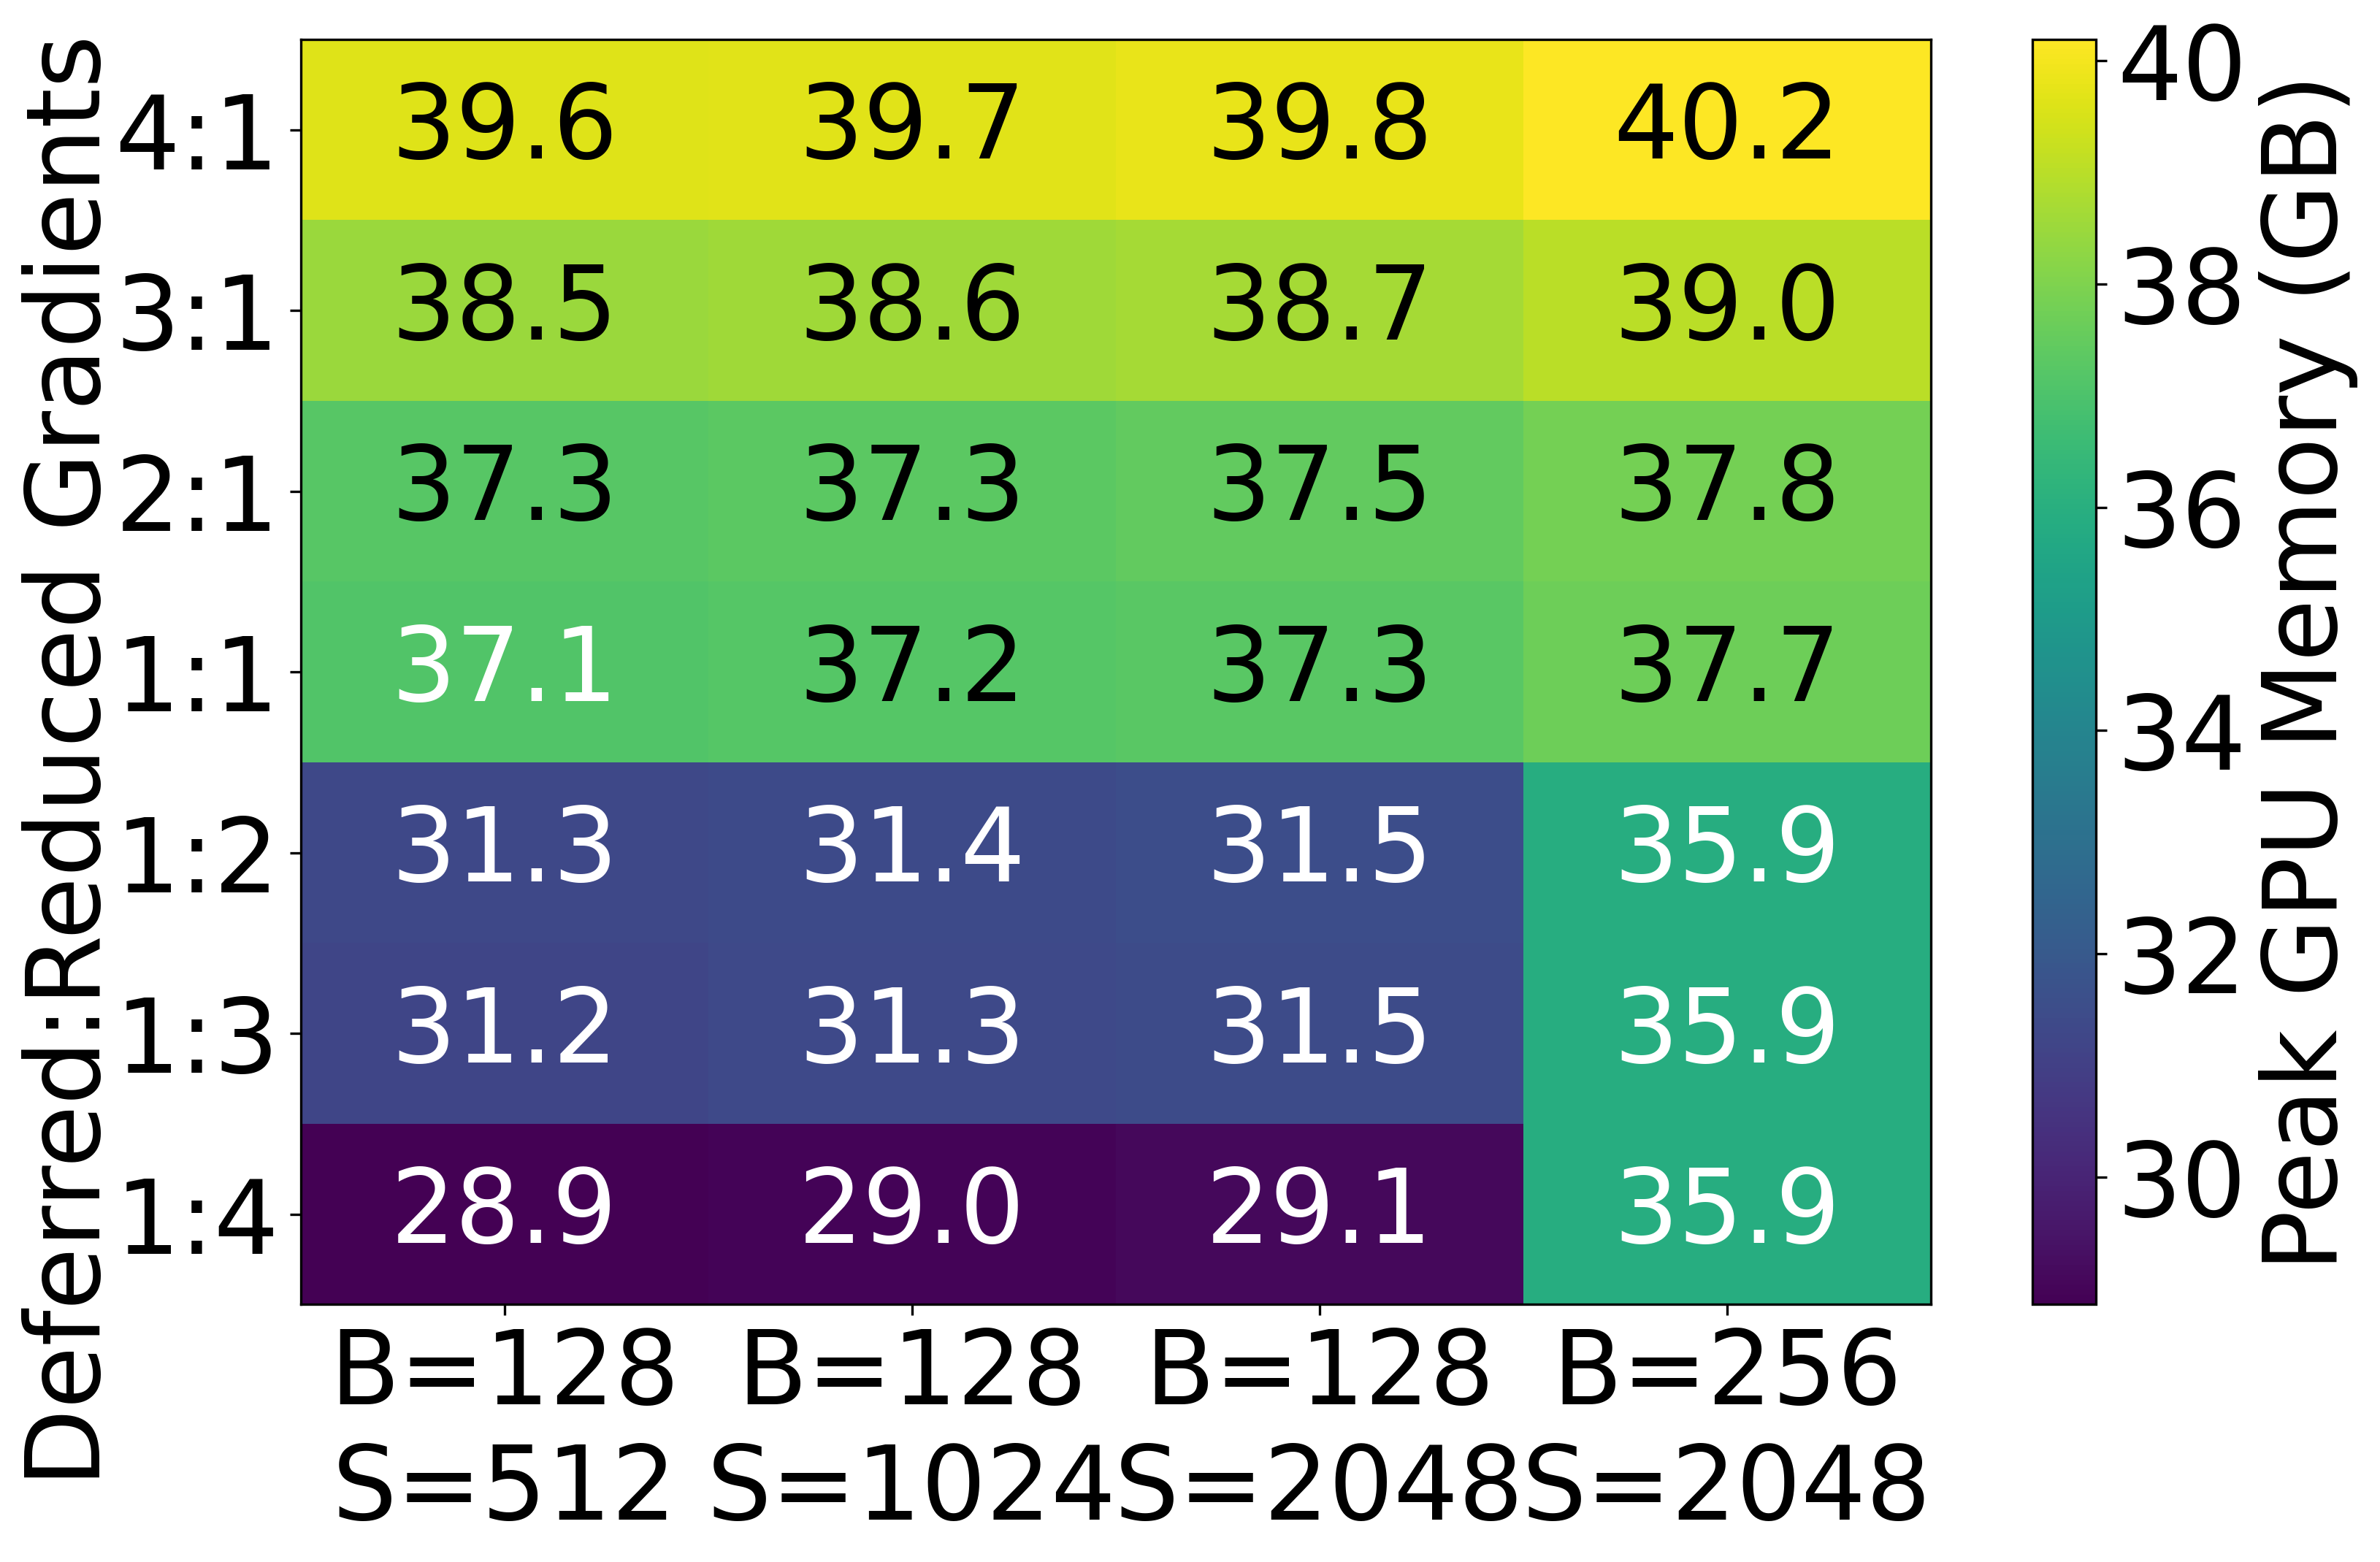
\includegraphics[width=\linewidth]{figures/strategy_4.0_ckpt_False_peak_gpu_mem_mb_heatmap.png}
    \vspace{-1.5em}
    \caption{Peak Memory (ZeRO-4)}
  \end{subfigure}
  \vspace{-0.5em}
  \caption{Configuration exploration of ZeRO-3.5 \& ZeRO-4.}
  \label{fig:zero_dse}
  % \vspace{-2em}
\end{figure}

As shown in Fig.~\ref{fig:zero_dse}(a), ZeRO-3.5's performance generally increases as the fraction of retained parameters grows, with larger gains under lighter computation loads. However, increasing the retained-parameter ratio can also raise peak memory usage. As shown in Fig.~\ref{fig:zero_dse}(b), when activation is small, the gathered parameters dominate peak memory, therefore, peak memory increases with the retained-parameter ratio. When activation is sufficiently large, the retained parameters can occupy the freed activation memory (Fig.~\ref{fig:FSDP}(c)), and retaining more parameters no longer increases peak memory.

Figure~\ref{fig:zero_dse}(c) shows that ZeRO-4 attains the best performance at a moderate deferred-gradient ratio (1:3). A low deferred ratio degenerates to ZeRO-3.5, while a high deferred ratio introduces excessive forward communication, which can overload the forward pass and reduce communication-computation overlap. As illustrated in Fig.~\ref{fig:zero_dse}(d), when activation is small, peak memory grows with the deferred-gradient ratio due to more retained gradient buckets during backward. When activation is large enough, peak memory becomes less sensitive to the deferred-gradient ratio where both deferred gradient buckets and retained parameters can be accommodated in the released activation memory (Fig.~\ref{fig:FSDP}(d) \& \ref{fig:zero_comparison}(g)).

\subsection{Search Analysis}
\label{sec:exp_search}

\name{}'s search process constructs a sequence of intermediate strategies that connect the initial strategy to the terminal one. As illustrated in Fig.~\ref{fig:zero_search}, under the data-monistic abstraction, each all-gather operation in ZeRO-3 creates a Weight Buffer CAT that collects weight shards from peer devices. The transition from ZeRO-3 to ZeRO-3.5 is a progressively delaying the release event of the Weight Buffer CAT during the backward pass until the corresponding forward layer is reached. At that point, the automatic management selects the Weight Buffer resident on the local device rather than all-gathering weights from other devices.

\begin{figure}[h]
  \centering
  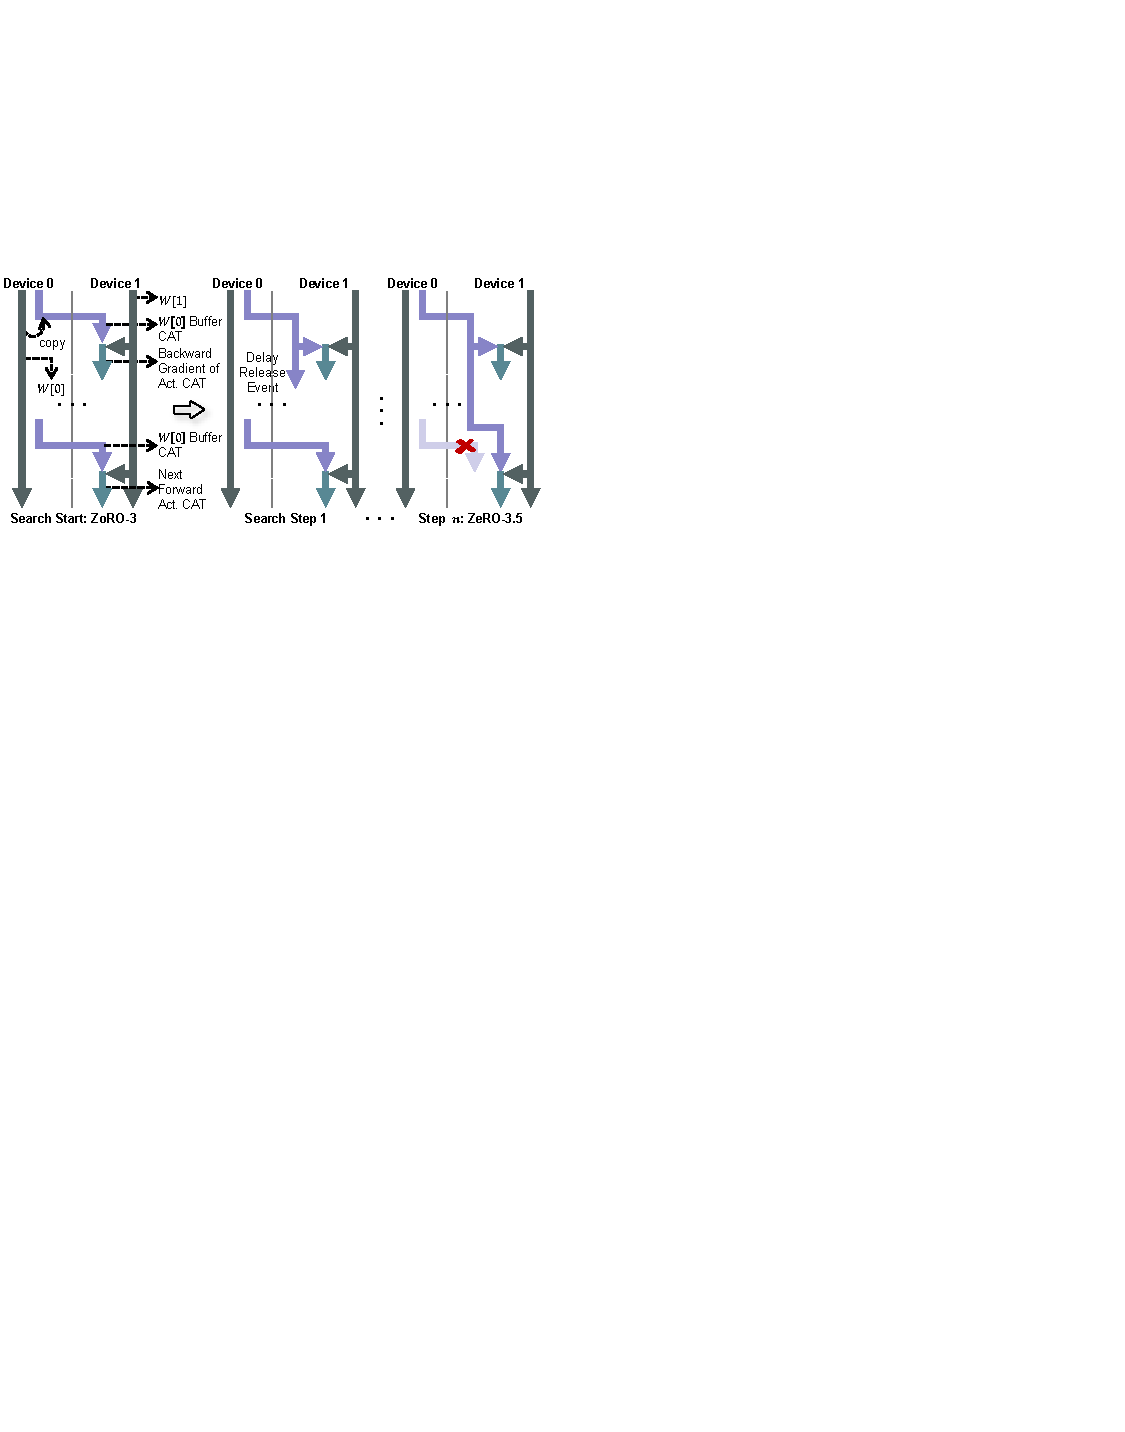
\includegraphics[width=1\linewidth]{figures/zero_search.pdf}
  \caption{The intermediate strategy during search from ZeRO-3 to ZeRO-3.5.}
    \label{fig:zero_search}
\end{figure} 

In our ZeRO search experiments, the event-potential function we use is: . We also incorporate a CAT's attraction to its dependencies into the accumulated potential of each dependent CAT. Fig.~\ref{fig:comprehensive_search2} shows the distribution of event potential across CATs for ZeRO-3 and ZeRO-3.5, highlighting the changes of the Weight Buffer CAT. We observe that, during the backward phase of the first accumulation step, two Weight Buffer CATs replace the Buffer CATs of the subsequent forward pass, resulting in a smaller accumulated potential.

\begin{figure}[h]
  \centering
  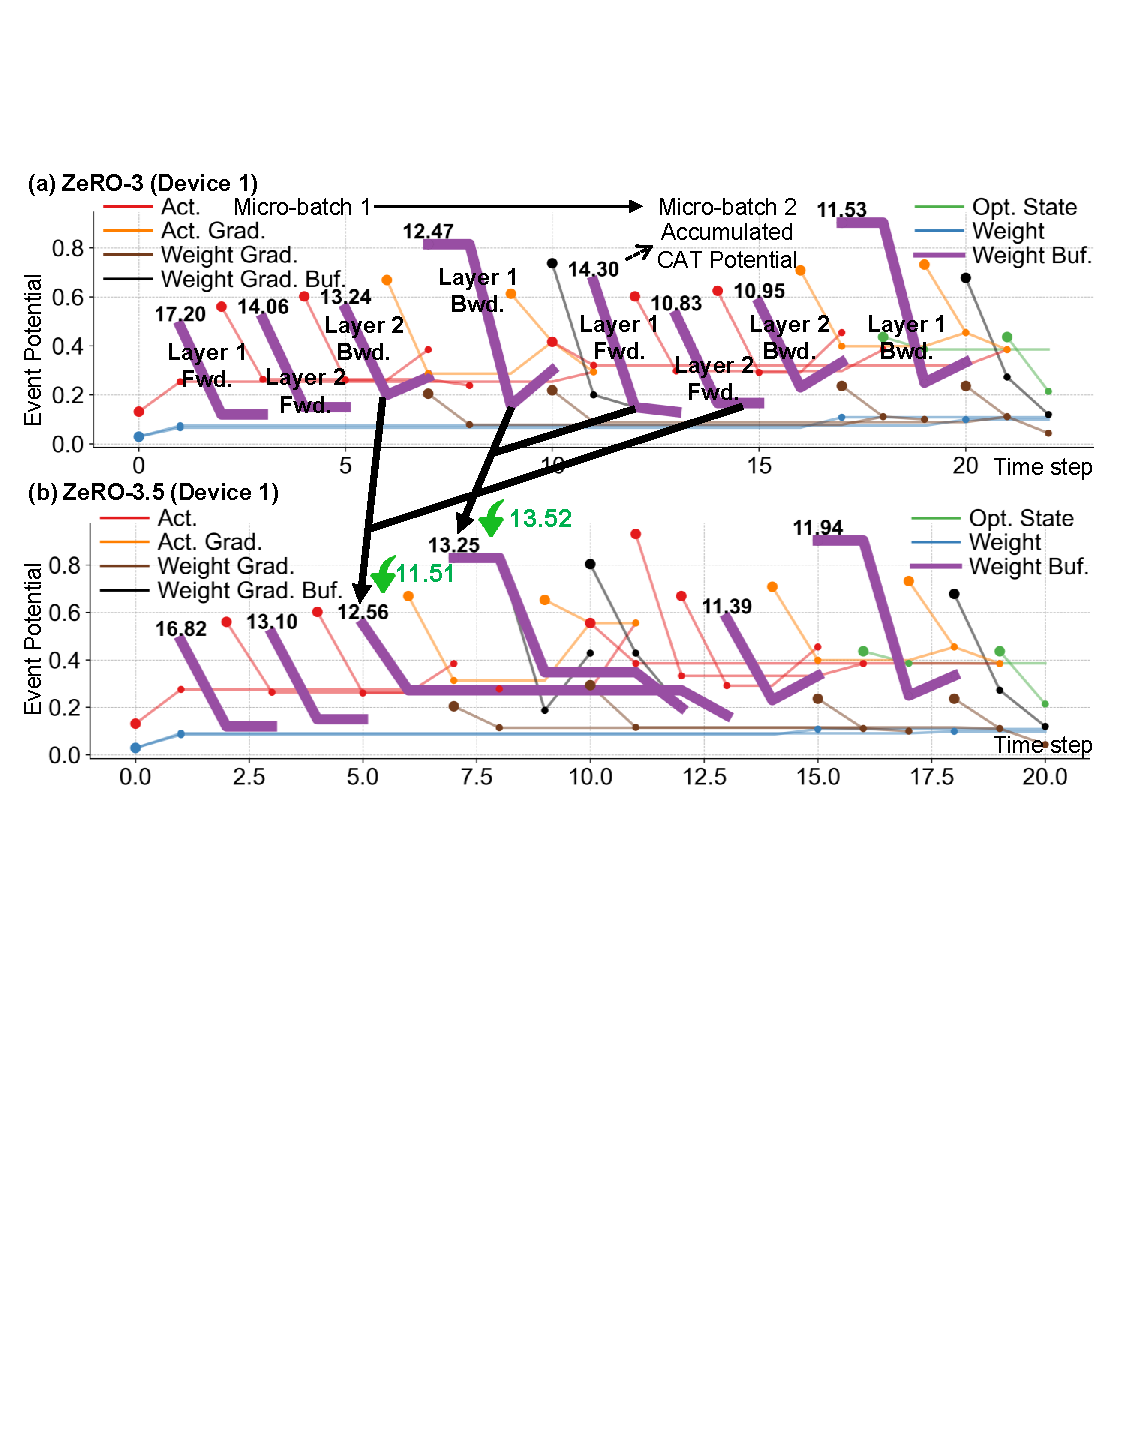
\includegraphics[width=1\linewidth]{figures/comprehensive_search_2.pdf}
  \caption{Potential distributions for (a) ZeRO-3 and (b) ZeRO-3.5. Both strategies are illustrated using a 2-layer, 2-accumulation-step, 4-device configuration.}
    \label{fig:comprehensive_search2}
\end{figure}

Fig.~\ref{fig:zero_search_potential}(a) further plots the accumulated potential of each Weight Buffer CAT along the trajectory from ZeRO-3 to ZeRO-3.5 (The accumulated CAT potential of intermediate strategies). With the defined potential function, this transition constitutes a natural potential-descent process, causing the high reachability of ZeRO-3.5. In contrast, attaining ZeRO-4 is more challenging. As shown in Fig.~\ref{fig:zero_search_potential}(b), deferring the backward Weight Gradient Buffer to the subsequent forward pass does not yield a monotonically decreasing communication load for many layers, while the memory footprint grows with deferral and the attraction rules cannot be applied. Consequently, optimizing the Weight Gradient Buffer within automated search primarily serves to reveal promising directions rather than directly producing the final ZeRO-4 strategy.

\begin{figure}[h]
  \centering
  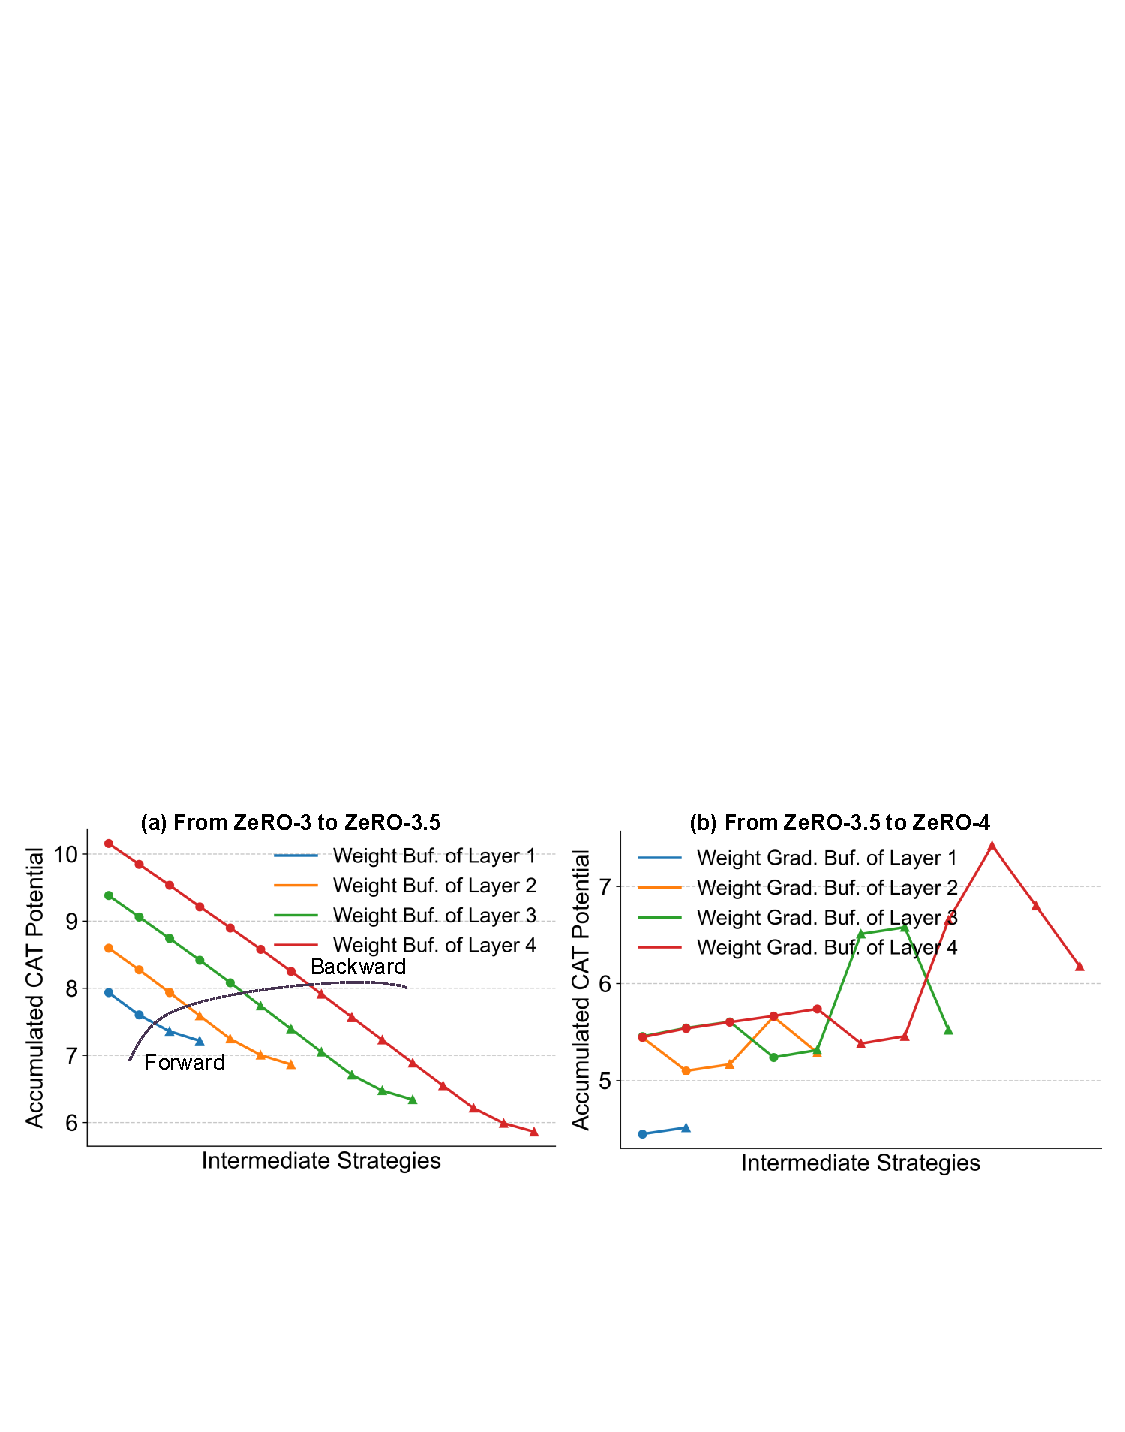
\includegraphics[width=1\linewidth]{figures/zero_search_potential.pdf}
  \caption{Search trajectory of weight buffer CAT (a) from ZeRO-3 to ZeRO-3.5. (b) from ZeRO-3.5 to ZeRO-4.}
    \label{fig:zero_search_potential}
\end{figure} 

\subsection{Comprehensive Exploration}
\label{sec:exp_offload}

\subsubsection{Seven search directions} 

\begin{figure}[h]
  \centering
  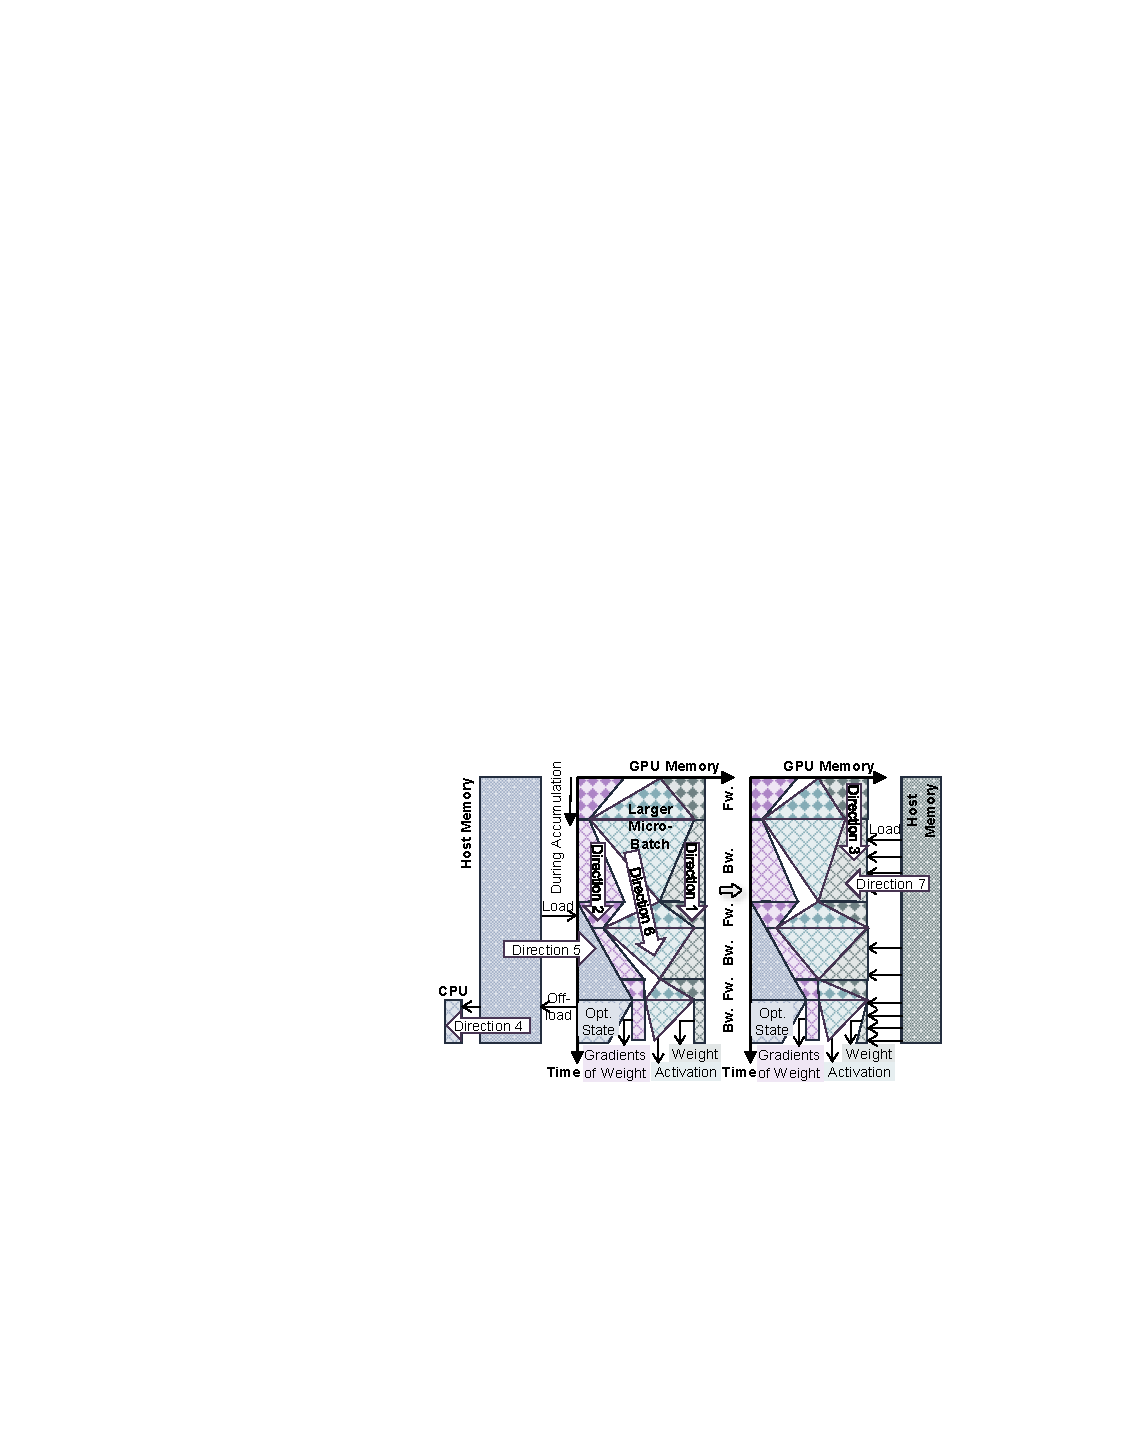
\includegraphics[width=0.9\linewidth]{figures/comprehensive_search_1.pdf}
  \caption{Comprehensive potential-descent directions discovered by \name{} starting from ZeRO-3. The seven directions span ZeRO improvement (1–3) and offload (4–7) optimizations, each targeting different computation-memory–communication trade-offs.}
    \label{fig:comprehensive_search1}
\end{figure}

Starting from ZeRO-3, our data-centric potential-based search identifies seven meaningful scheduling optimization directions across various model and hardware configurations. These seven directions are comprehensively illustrated in Figure~\ref{fig:comprehensive_search1}. Directions 1 through 3 involve the GPU performing all storage and computation. \textbf{Direction 1} represents the ZeRO-3.5 strategy, i.e., delaying the release of backward weights. \textbf{Direction 2} represents the ZeRO-4 strategy, i.e., delaying the gradient reduce-scatter. \textbf{Direction 3} entails retaining a portion of forward weights for the backward pass, thereby increasing memory usage to reduce backward communication, which serves as an intermediate strategy between ZeRO-2 and ZeRO-3 (ZeRO-2.5). Directions 4 through 7 involve offload strategies:
\textbf{Direction 4:} Conventionally storing optimizer states in host memory (or SSD), with the CPU performing optimizer state updates.
\textbf{Direction 5:} Pre-loading optimizer states stored in host memory onto the GPU for updates.
\textbf{Direction 6:} Employing a larger micro-batch size before optimizer state pre-loading, and a smaller size after loading.
\textbf{Direction 7:} Off-loading weights to host memory.


\subsubsection{New Offload strategy} 

Guided by the search direction, we evaluate the new offload strategy on real hardware. \weihao {TODO}

\textbf{Baseline Offload (ZeRO-style).} 
\junfeng{Baseline is ZeRO or ZeRO-offload ? These two are both important comparable strategies}
Conventional offload techniques store optimizer states in host memory (DRAM) or SSD. During backpropagation, gradients on the GPUs are transferred to the host, the CPU applies the optimizer update on the host-resident states, and the updated weights are sent back to the GPUs (Direction 4). End-to-end iteration time is frequently limited by host--device bandwidth and CPU throughput; to mitigate these bottlenecks, ZeRO-Infinity-style deployments sometimes provision multiple high-performance CPUs per GPU cluster.

\textbf{Preload-then-discard Offload Strategy (PTD-offload).} The strategies discovered by \name{} exploit large GPU memory to pre-load optimizer states onto the GPUs ahead of the final backward pass within a batch, perform the optimizer updates directly on GPUs, and immediately discard the optimizer states thereafter (Direction 5). In parallel, the CPU executes a redundant optimizer-state update, but the GPUs do not wait for the CPU results; they proceed to the next batch's gradient accumulation and later pre-load the CPU-updated states when available. In addition, we adopt a variable micro-batch-size policy to co-optimize memory and throughput: when optimizer states are not resident on GPUs, we use a larger micro-batch size to better amortize communication and increase utilization; when optimizer states occupy GPU memory, we reduce the micro-batch size to free space for the states (Direction ).

\textbf {Setup}
Fig.~\ref{fig:off_load_strategy} presents a performance comparison of our strategy and the ZeRO-style offload strategies across two model sizes and three distinct hardware configurations on 8 GPUs. The total training batch size and sequence length here are fixed at 64 and 2048 for each GPU. For each configuration, we use the largest micro batch size that does not cause out-of-memory(OOM) to maxiumize the utilization of GPUs. Due to memory constraints, we enable gradient checkpointing for the 32B model, allowing us to maintain a minimum batch size of $1$ for ZeRO3.  We do not incorprate ZeRO2 here for it cause OOM in all configurations. 

\textbf{ZeRO3 v.s. ZeRO3-offload}
As shown in Fig.~\ref{fig:off_load_strategy},  in low-bandwidth configurations (e.g., H800-PCIe), the throughput of ZeRO-3 is predominantly bottlenecked by its communication overhead. Applying memory offloading to ZeRO-3 allows for larger batch sizes, which can potentially increase throughput. However, for the 14B model, the computational cost incurred by the weight update step on the CPU is significant, resulting in only a marginal net improvement in overall throughput.In contrast, for the 32B model utilizing Gradient Checkpointing, offloading proves highly effective: it enables a substantial increase in the batch size (e.g., from 1 to 16), thereby yielding a significant improvement in overall training throughput.

\textbf{PTD-offload}
The PTD-offload technique effectively combines the benefits of ZeRO and offloading. It operates by initially utilizing ZeRO-2 with a large batch size during the early accumulation steps. It then transitions (degrades) to ZeRO-3 only after initiating the preloading of optimizer states.

This segmented approach achieves superior computation-communication overlap and eliminates the performance cost associated with applying computations on the slower CPU, resulting significant performance improvements across most settings. The exception is the H20 configuration, which features faster communication bandwidth and larger memory (implying larger batch sizes and higher compute utilization). In this specific setting, the advantage gained by our model is relatively smaller.

\begin{figure}[h]
  \centering
  \begin{subfigure}{\linewidth}
    \centering
    
\includegraphics[width=0.9\linewidth]{figures/legend_offload.png}
    \vspace{-0.2em}
  \end{subfigure}
  \begin{subfigure}{0.49\linewidth}
    \centering
    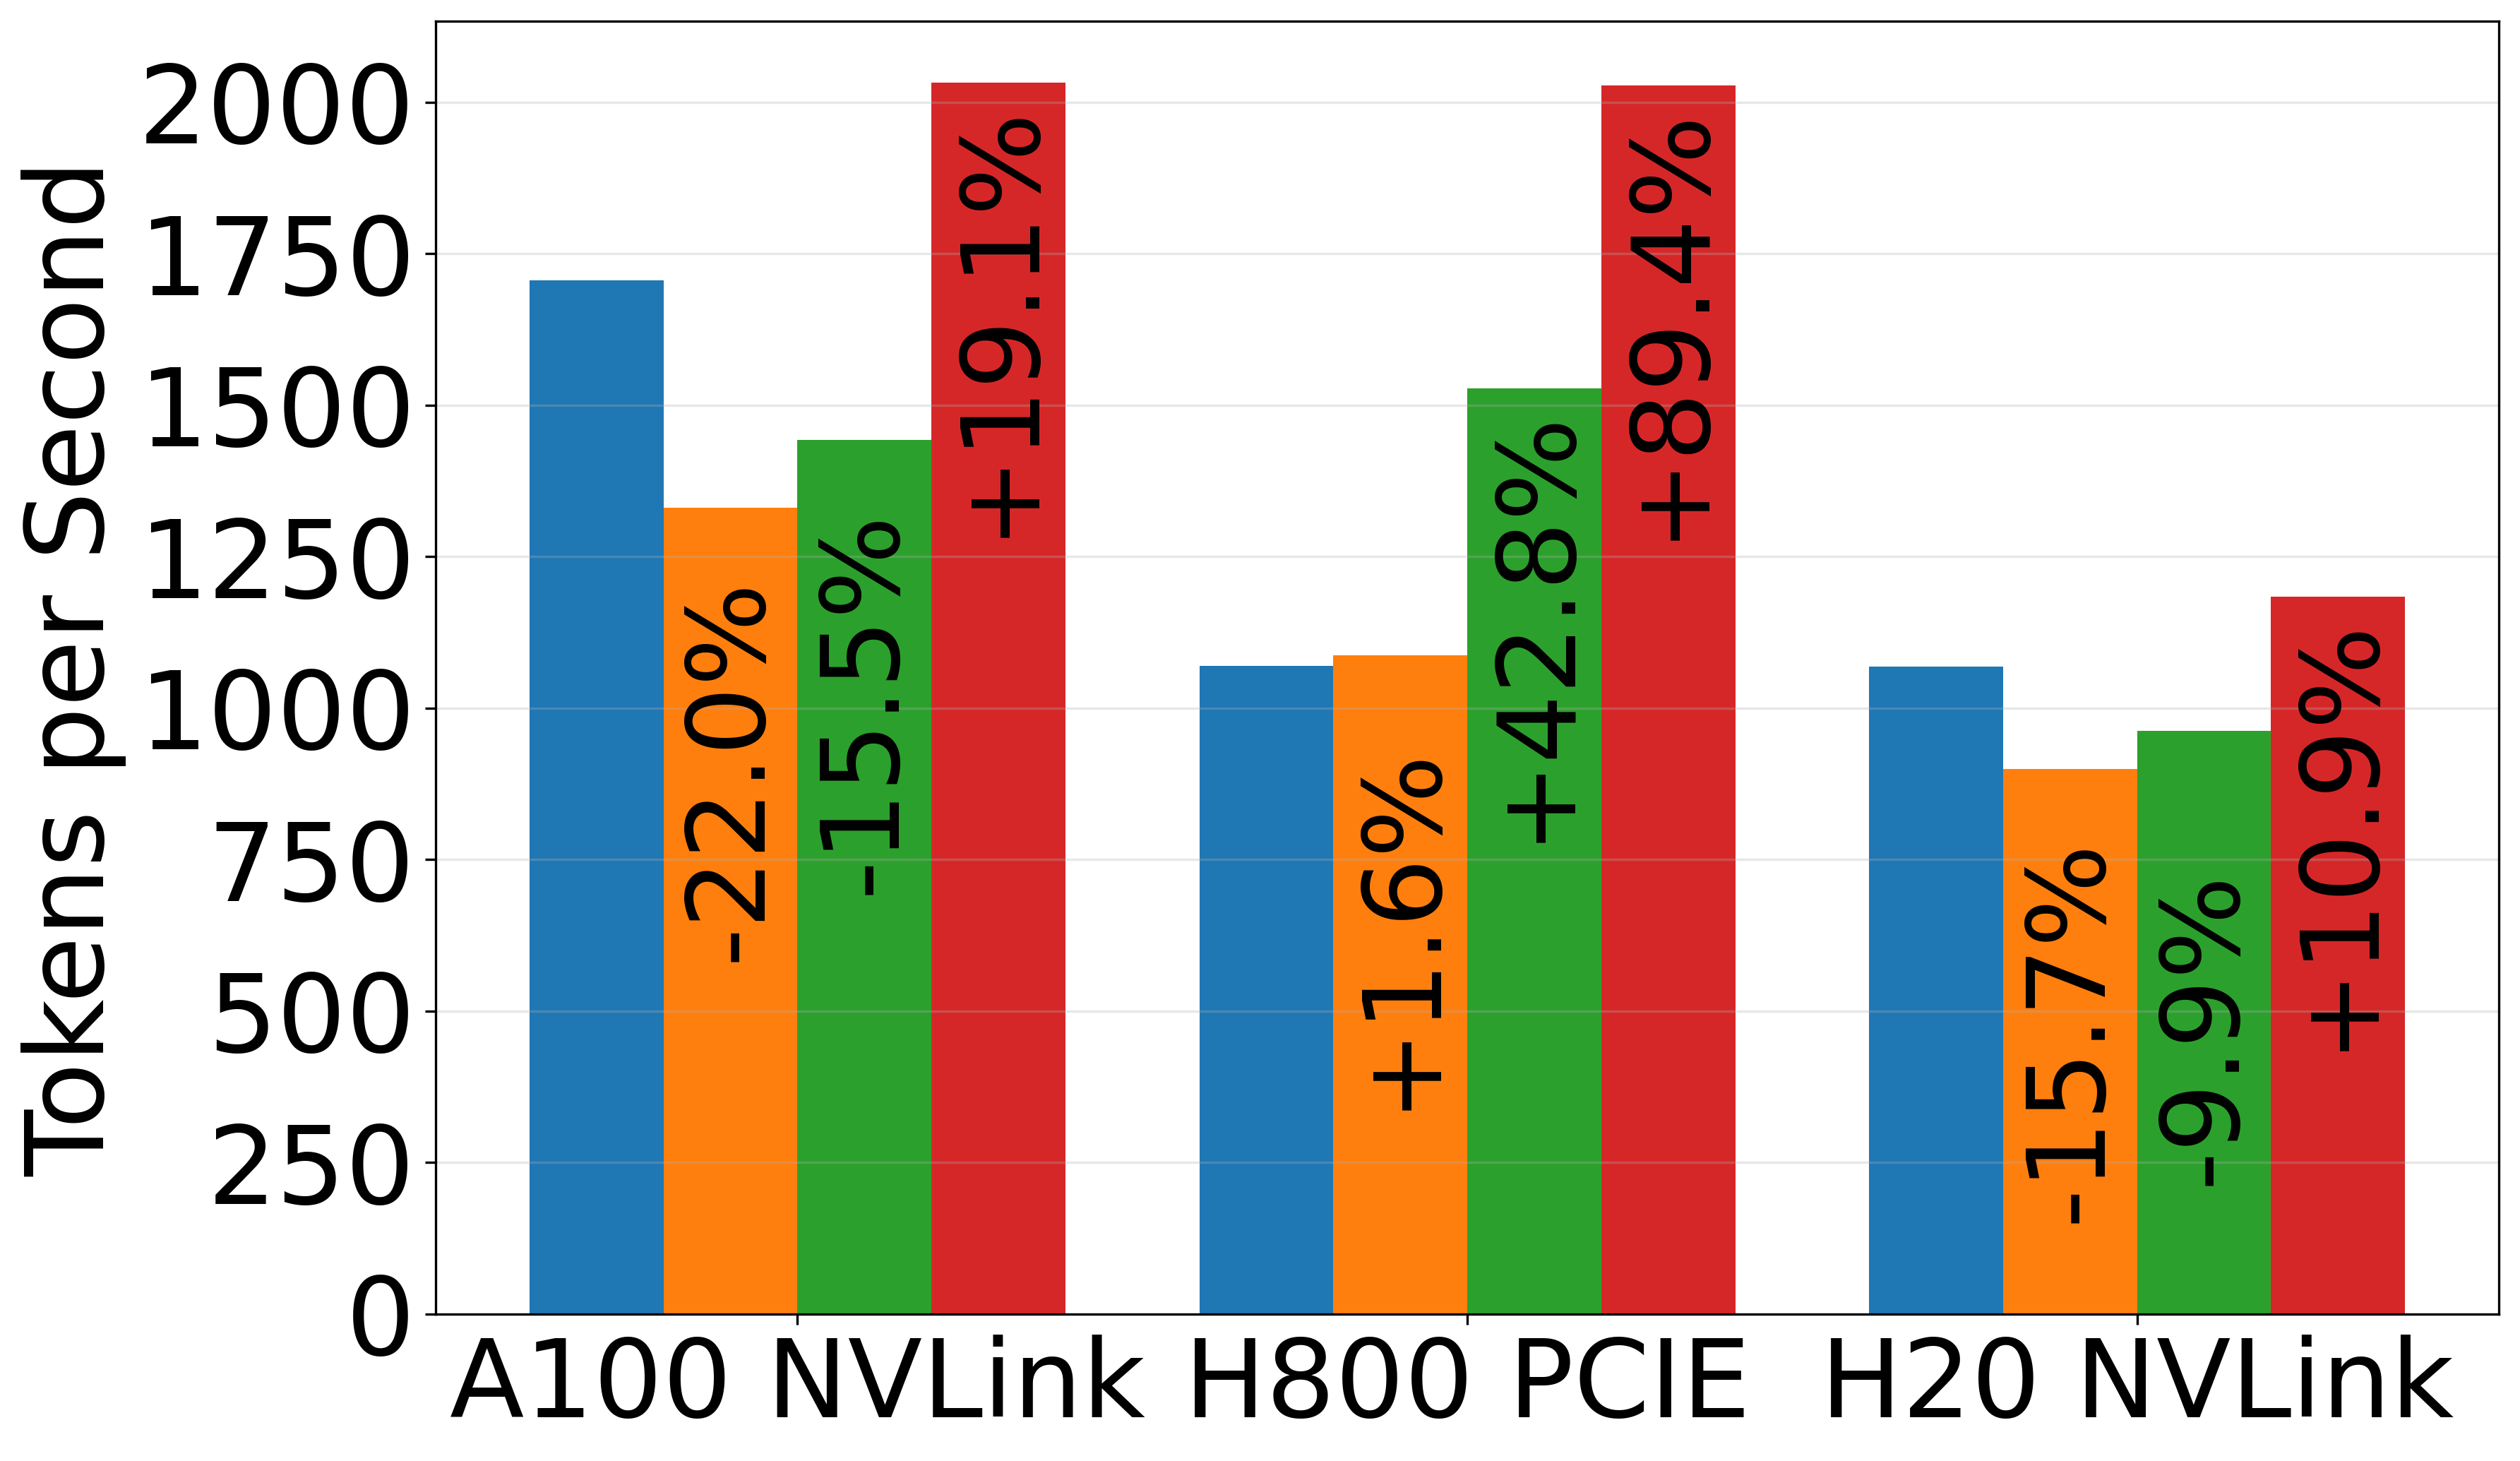
\includegraphics[width=\linewidth]{figures/offload_comparison_Qwen3-14B.png}
    \vspace{-1.5em}
    \caption{Qwen3-14B}
  \end{subfigure}
  \begin{subfigure}{0.49\linewidth}
    \centering
    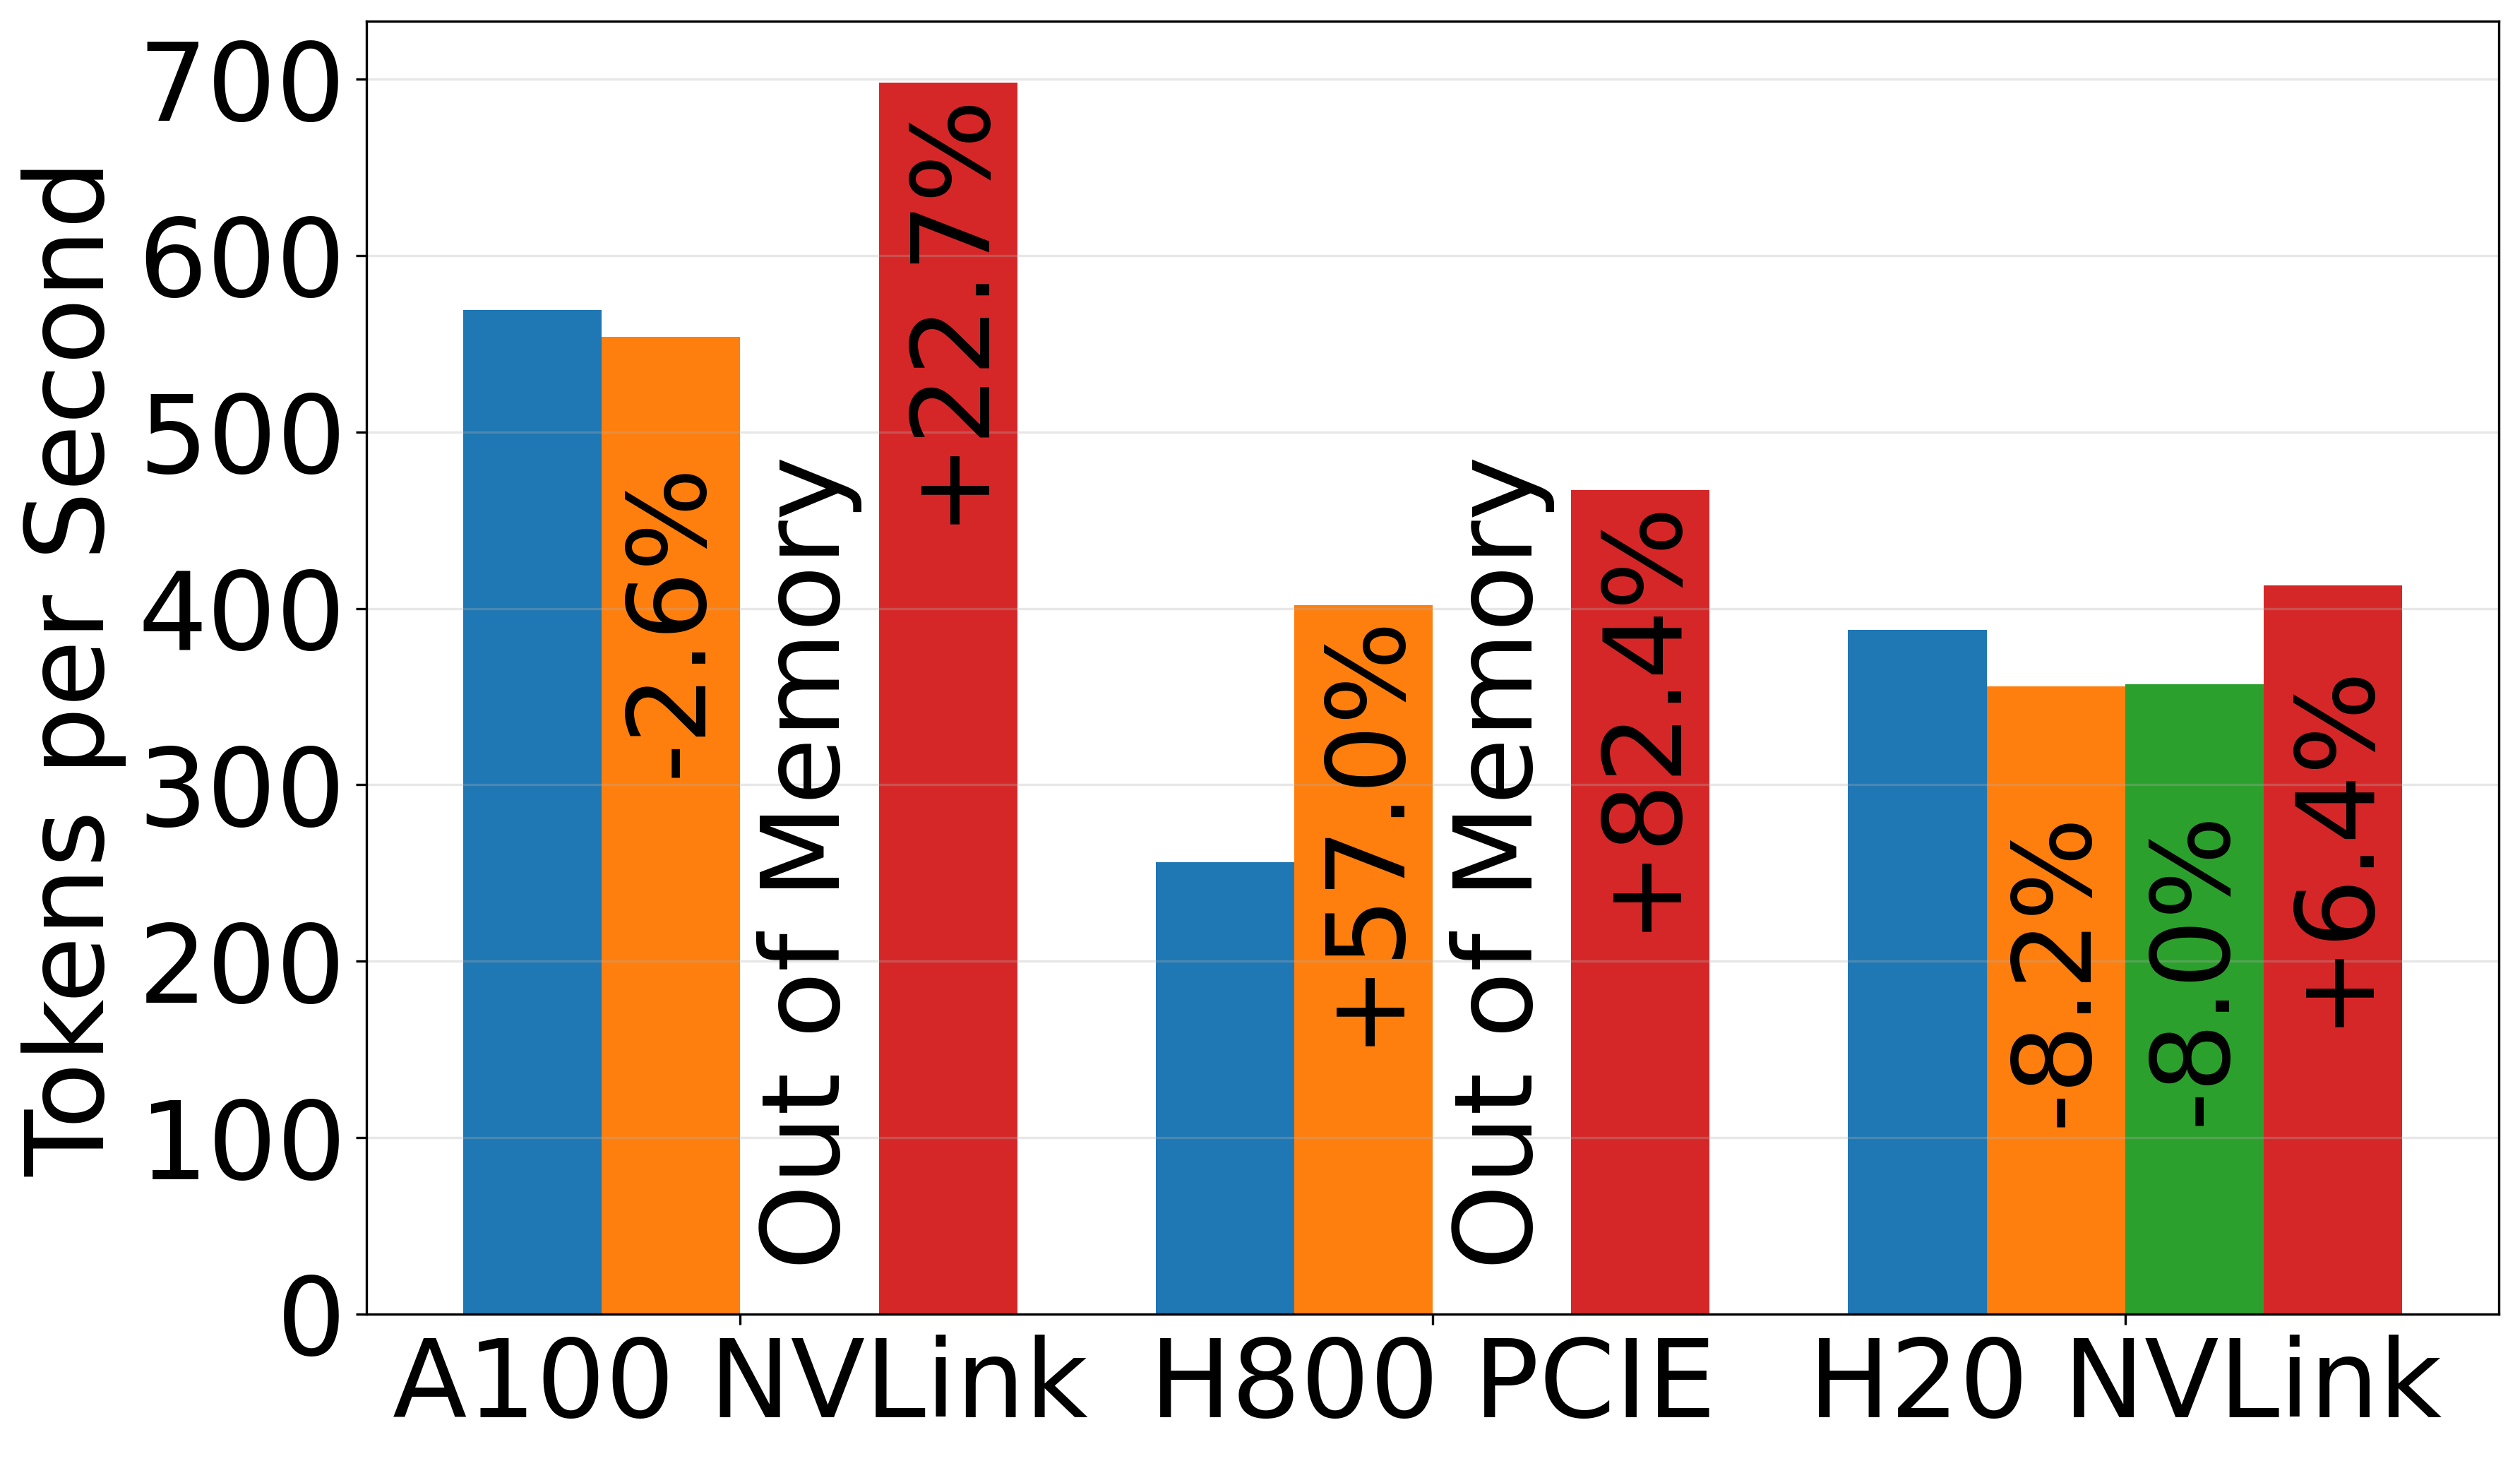
\includegraphics[width=\linewidth]{figures/offload_comparison_Qwen3-32B.png}
    \vspace{-1.5em}
    \caption{Qwen3-32B}
  \end{subfigure}
  \vspace{-0.5em}
  \caption{Offload strategy comparison (baseline: ZeRO-3).}
  \label{fig:off_load_strategy}
\end{figure}

\section{Conclusion}

In this paper, we present \name{}, a data-monistic abstraction for distributed training that unifies the representation of data and computation. By introducing the concept of Constraint-Aware Tensors (CATs) and a set of data-centric primitives, \name{} enables the declarative specification of complex parallelization strategy spaces. We also propose a constraint-based potential descent search algorithm that systematically explores this vast strategy space, discovering efficient parallelization plans that outperform existing methods. However, \name{} focuses on high-level distributed scheduling and does not extend to micro-architectural optimizations tightly coupled with hardware, such as PagedAttention. Furthermore, this paradigm shift introduces significant implementation challenges, and a full end-to-end system remains an area for future work. In addition, more efficient search algorithms could be further explored.

%-------------------------------------------------------------------------------
\bibliographystyle{plain}
\bibliography{ref.bib}

\appendix

\section{Data-Centric Primitives in \name{}}
\label{sec:all_primitives}

\begin{table*}[h]
\centering
\resizebox{\textwidth}{!}{%
\begin{tabular}{p{0.4\textwidth}p{0.6\textwidth}}
\toprule
Primitives                             & Usage \\ \midrule
\texttt{split(tensor, split\_vector, split\_tensors)}         & \texttt{tensor} represents the tensor to be partitioned. \texttt{split\_vector} represents the vector guiding how to partition \texttt{tensor}. \texttt{split\_tensors} are the result tensors. \\
\texttt{assign(tensor, device)}        & Assign \texttt{tensor} to \texttt{device}. \\
\texttt{copy(src\_tensor, device, dst\_tensor, path)} & Copy \texttt{src\_tensor} from its current device to \texttt{device}. The copied tensor on \texttt{device} can be accessed through the pointer \texttt{dst\_tensor}. \texttt{path} represents the copy path. \\
\texttt{cut(src\_tensor, device, dst\_tensor, path)} & Cut \texttt{src\_tensor} from its current device to \texttt{device}. The moved tensor on \texttt{device} can be accessed through the pointer \texttt{dst\_tensor}. \texttt{path} represents the cut path. After cut, \texttt{src\_tensor} will be freed from memory.        \\
\texttt{reduce(src\_tensors, device, dst\_tensor, path)} & Reduce \texttt{src\_tensors} into \texttt{dst\_tensor}. The reduction result will be placed on \texttt{device}. \texttt{path} represents the reduction path.     \\
\texttt{redirect(tensor1, tensor2, tensor3)} & Redirect the data dependencies between \texttt{tensor1} \& \texttt{tensor3} to \texttt{tensor2} \& \texttt{tensor3}.                                        \\
\texttt{order(event1, event2)}        & Enforce temporal order between \texttt{event1} and \texttt{event2}.  \texttt{event1} executes before \texttt{event2}.                                                                                      \\ \bottomrule
\end{tabular}%
}
\caption{Data-centric primitives for parallelization space construction in \name{}.}
\label{tab:primitives}
\end{table*}

\section{Details of ZoRO strategies}

FSDP is a widely-adopted data parallelism strategy that coordinates computation and data movement. It shards model parameters, gradients, and optimizer states across devices to reduce memory. During training, each device holds only a shard of the weights. For a forward pass, a device gathers the full parameters for the current layer, performs the computation, and then discards the full parameters, keeping only its shard. For the backward pass, gradients are computed locally and then reduced and sharded directly to the target devices using a reduce-scatter operation, avoiding redundant storage. This sharding strategy is often described in levels, inspired by the ZeRO (Zero Redundancy Optimizer) framework~\cite{rajbhandari2020zero}. ZeRO-1 shards optimizer states, ZeRO-2 adds gradient sharding, and ZeRO-3 (the typical FSDP implementation) shards parameters as well for maximum memory savings. Algorithm \ref{alg:fsdp} shows how \name{}'s primitives can represent the core of ZeRO-2/3. 

Figure \ref{fig:FSDP}(a-b) illustrates the approximate changes in storage and communication volume during training for ZeRO-2 and ZeRO-3. Figure \ref{fig:FSDP}(a) illustrates the storage and communication changes in ZeRO-2. During the forward pass, activation storage on each device increases as new activations are generated. In the backward pass, activations are consumed and released. In the final backward step of a batch, each device performs a reduce-scatter of gradients of weights with other devices to update its optimizer state and the corresponding weight shard; old weights can then be discarded. To balance communication load, ZeRO-2 typically performs an all-gather of new weights at the start of the next batch's first forward pass. Assuming each layer's forward computation takes one step and each device transmits one block of data per weight or gradient transfer, the communication volume per device during the first forward is 1 block/step. In the final backward, only gradients of weights are communicated, and since each backward layer takes about twice as long as a forward layer (2 steps), the average communication volume is 0.5 block/step. In practice, multiple gradient accumulation steps are performed; Figure \ref{fig:FSDP} shows only one accumulation, but this process is usually repeated many times and dominates training cost. During accumulation, since ZeRO-2 stores all weights on each device, only the reduce-scatter of weight gradients is needed during backward, with communication volume calculated as 0.5 block/step. ZeRO-3, by sharding the weights, achieves greater memory savings compared to ZeRO-2, as each device only stores a portion of the weights. However, during gradient accumulation, every forward and backward pass for each layer requires an all-gather operation to assemble the complete weights on each device before computation. Consequently, the average communication volume per device for both forward and backward passes is 1 block per step, which becomes the primary performance bottleneck in ZeRO-3. If a strategy could be found that achieves the memory savings of ZeRO-3 while approaching the communication efficiency of ZeRO-2, it would be highly valuable.

\section{Details and Concerns About Search Algorithm}
\label{sec:search_details}

1. Symmetry Constraints: To improve search efficiency and reduce highly irregular solutions, symmetry constraints can be introduced into the search algorithm. That is, CATs with symmetric constraint vectors are treated as equivalent, and their scheduling actions are bound together during the search process.

2. Collectivity and Individuality of Potential: In the main text, we describe the calculation of potential as a global property, implying that the potential landscape is identical for each CAT. However, this is not strictly the case. Some metrics that influence "potential," such as memory pressure or overall computation latency, are indeed global. However, each CAT may also be subject to individualized constraints that exert personalized pressure, such as the requirement to arrive at a specific device before a certain event to synchronize with another CAT. As the event approaches, the pressure for the CAT to flow toward that device increases. Therefore, the movement of each CAT is not determined solely by the global potential.

3. In the absence of the hole mechanism described in the main text, it is not possible to constrain non-domain strategy spaces. Thus, by default, our search algorithm allows free exploration of these strategy spaces.

4. The search algorithm should be guided by certain heuristics. For example, in the absence of pressure-driven guidance, a CAT may simply remain on its current device without being released. Such heuristics can help the algorithm discover anticipated strategy optimization directions.

5. Two-level Heuristic Descent: In theory, it is possible to treat the constraint vector of a CAT as a whole and perform heuristic descent on it. However, finding the optimal descent direction would require enumerating all possible next-step transformations of the constraint vector, which is computationally infeasible due to the combinatorial explosion when multiple event points are involved. To address this, we adopt a two-level heuristic descent approach. At the first level, we perform local heuristic descent for each event point, identifying the optimal descent direction for each (i.e., applying a coordinate descent algorithm to the constraint vector). At the second level, we combine these locally optimal descent directions to determine the overall optimal descent direction for the entire constraint vector.

6. It is not accurate to state that the search process continuously refines the strategy space, as the potential descent algorithm merely iterates from one strategy solution to another without altering the strategy space itself. However, it is correct to say that the process of writing primitives refines the strategy space. In addition, a refinement engine exists within the search algorithm—using techniques such as constraint propagation—to prune the strategy space.

\section{Implementation Details}
\label{sec:implementation_details}

%%%%%%%%%%%%%%%%%%%%%%%%%%%%%%%%%%%%%%%%%%%%%%%%%%%%%%%%%%%%%%%%%%%%%%%%%%%%%%%%
\end{document}
%%%%%%%%%%%%%%%%%%%%%%%%%%%%%%%%%%%%%%%%%%%%%%%%%%%%%%%%%%%%%%%%%%%%%%%%%%%%%%%%

%%  LocalWords:  endnotes includegraphics fread ptr nobj noindent
%%  LocalWords:  pdflatex acks
